% ============================================================================
% Master page - setup document
% ============================================================================

% === Impostazione del documento ==========================
\documentclass[12pt,a4paper,twoside,english,hidelinks]{book}
\pagenumbering{arabic}
\usepackage{setspace}
\onehalfspace
\usepackage[a-1b]{pdfx}
%\usepackage{ucs} % this is already implied by pdfx
\usepackage[utf8]{inputenc}
\usepackage[LGR,T2A,T1]{autofe}
\usepackage[pdfa]{hyperref}
\usepackage{blindtext}
\usepackage{lmodern}
\usepackage{minted}

% === Regolazione dei margini =============================
\addtolength{\oddsidemargin}{30pt}
\addtolength{\evensidemargin}{-30pt}
\usepackage{fancyhdr}
\usepackage{multirow}
\usepackage{multicol}
\usepackage[section]{placeins}

% === Impostazione dei font ===============================
\usepackage[T1]{fontenc}
\usepackage[english]{babel}
\usepackage{ae}
\usepackage{relsize}
\usepackage{csquotes}
\usepackage{amsmath}
\usepackage{amsfonts}
\usepackage{mathdots}
\usepackage{mathtools}
\usepackage{pagecolor}
\usepackage{lettrine}
\usepackage{siunitx}
\hypersetup{
	bookmarksnumbered=true,
	linkcolor=black,
	citecolor=black,
	urlcolor=black,
}
\usepackage{verbatim}
\usepackage{alltt,footnote}
\DeclareMathOperator{\sgn}{sgn}
\DeclarePairedDelimiter{\abs}{\lvert}{\rvert}
\DeclarePairedDelimiter{\norma}{\lVert}{\rVert}
\usepackage{amssymb}
\usepackage[defblank]{paralist}


% === Integrazione delle figure ===========================
\usepackage{graphicx}
\graphicspath{{./imgs/}{./hardware/imgs/}{./software/imgs/}{./neuralnetworks/imgs/}}
%\renewcommand{\figurename}{Fig.}
\usepackage{caption}
\captionsetup[figure]{labelfont=bf}
\newcommand*{\captionsource}[2]{%
  \caption[{#1}]{%
    #1%
    \\\hspace{\linewidth}%
    \textbf{Source:} #2%
  }%
}
\usepackage{subfig}
\usepackage{xcolor}

%
% === Per gli algoritmi ===================================
\usepackage{algorithmicx}
\usepackage[ruled]{algorithm}
\usepackage{algpseudocode}

% === Per le tabelle ======================================
\usepackage{tabularx}
\usepackage{colortbl}

%==Per le figure latex======================================
%Package e librerie per TikZ e PGF, le librerie non sono tutte necessarie a questo documento LATEX.
\usepackage{tikz,fp,ifthen,fullpage}
\usepackage{pgfmath}
\usetikzlibrary{decorations.pathmorphing,backgrounds,fit,calc,through}
\usetikzlibrary{arrows, automata, positioning}
\usetikzlibrary{shapes,decorations,shadows}
\usetikzlibrary{fadings}
\usetikzlibrary{patterns}
\usetikzlibrary{mindmap}
\usetikzlibrary{decorations.text}
\usetikzlibrary{decorations.shapes}
\usepackage{pgfplots}
\usepgfplotslibrary{colorbrewer}
\usepgfplotslibrary{patchplots}
\pgfplotsset{compat=1.13}
\usepgfplotslibrary{units} % to add units easily to axis
\usepgfplotslibrary{fillbetween} % to fill inbetween curves
\usepgfplotslibrary{colormaps} % to create colormaps
\pgfplotsset{width=12.2cm, height=7cm}
\pgfplotsset{compat=newest} %(making it only compatalbe with
%new releases of pgfplots)
\pgfdeclarehorizontalshading{visiblelight}{50bp}{
color(0.00000000000000bp)=(violet);
color(8.33333333333333bp)=(blue);
color(16.66666666666670bp)=(cyan);
color(25.00000000000000bp)=(green);
color(33.33333333333330bp)=(yellow);
color(41.66666666666670bp)=(orange);
color(50.00000000000000bp)=(red)
}%

%== Per APDL e linguaggi======================================
\usemintedstyle{manny}
\usepackage{listings}
\lstset{%
  breaklines=true,
  breakatwhitespace=true,
}
\definecolor{bg}{HTML}{282828} % from https://github.com/kevinsawicki/monokai
\definecolor{codeBlue}{RGB}{0,0,255}
\definecolor{codeGreen}{RGB}{0,128,0}
\definecolor{codePurple}{RGB}{128,0,255}
\definecolor{codeOrange}{RGB}{255,128,128}
\definecolor{codePink}{RGB}{255,0,255}
\definecolor{codeGray}{rgb}{0.5,0.5,0.5}
\definecolor{aliceblue}{rgb}{0.94, 0.97, 1.0}
\definecolor{babyblueeyes}{rgb}{0.63, 0.79, 0.95}
\definecolor{light-gray}{gray}{0.95}
\definecolor{airforceblue}{rgb}{0.36, 0.54, 0.66}
\definecolor{amber}{rgb}{1.0, 0.75, 0.0}
\definecolor{amethyst}{rgb}{0.6, 0.4, 0.8}
\definecolor{applegreen}{rgb}{0.55, 0.71, 0.0}
\definecolor{arsenic}{rgb}{0.23, 0.27, 0.29}
\definecolor{bananayellow}{rgb}{1.0, 0.88, 0.21}
\definecolor{beaver}{rgb}{0.62, 0.51, 0.44}
\definecolor{ceruleanblue}{rgb}{0.16, 0.32, 0.75}
\definecolor{gold(web)(golden)}{rgb}{1.0, 0.84, 0.0}

%========================================
% TESTO DELLA TESI
%========================================
\begin{document}
	% === Frontespizio ====================================
	\pagestyle{empty}
	%%%%%%%%%%%%%%%%%%%%%%%%%%%%%%%%%%%%%%%%%%%%%%%%%%%%%%%%%%%
% Frontespizio
%%%%%%%%%%%%%%%%%%%%%%%%%%%%%%%%%%%%%%%%%%%%%%%%%%%%%%%%%%%
\begin{titlepage}
 \begin{center}
 
\includegraphics[width=3.5cm]{unitn}\\
 \vspace{1.5em}
 {\Large \textsc{University of study of Trento}}\\
 \vspace{1.5em}
 {\Large \textsc{Department of Industrial Engineering}}\\
 \vspace{4em}
 {\normalsize Master of Science in Mechatronics Engineering}\\
 \vspace{1.5em}
 {\Large \textsc{Mechanical design and machine elements}}\\
 \vspace{4em}
 {\LARGE\textbf{
 	Report homework
 }}\\
 \end{center}

\vskip 2.0cm
\vskip 2.0cm
 \begin{center}
 \begin{tabular}{c c c c c c c c}
 Professor & & & & & & & Candidate \\[0.2cm]
 \large{Prof. Brunelli Davide} & & & & & & & \large{Francesco Argentieri}\\[0.4cm]
  & & & & & & & ID 183892\\[0.2cm]
% \large{Dott. Egidio Labbate}& & & & & & &\\
 \end{tabular}
 \end{center}

\vskip 1.5cm
\begin{center}
{\normalsize academic year 2018/2019}
\end{center}
\end{titlepage}

\clearpage{\pagestyle{empty}\cleardoublepage}

	\chapter*{Abstract}
\label{chap:abstract}
%
%
\lettrine[lines=3]{T}{he aim} of this thesis is to increase the capabilities of
an Unmanned Aerial Vehicles (UAVs) using convolutional neural networks for
classification and object detection from images captured by the camera.
In recent times, the use of UAVs has increased both in the military and civilian
fields, such as for example in traffic control, surveillance, deliveries,
photography and exploration.
Within the UAV family, helicopters are preferred to fixed-wing aircraft
especially for their vertical take-off and landing capacity, and also for their
manoeuvrability.
These are used in activities where environments and circumstances are dangerous
to humans.
In parallel successes of deep learning techniques in solving many complex tasks
such as planning, localization, control and perception by starting from sensor
data acquired in real environments make it suitable in autonomous robotic
applications.\\
The development of dedicated hardware and software such as CUDA for Nvidia GPUs
which shows best performances in computer vision speech recognition signal
signal processing applications and so on.\\
A further aspect taken into consideration is the continuous evolution in the
field of Information Technology (IT) driven by the continual request for
decreasing capacity and costs.
So embedded systems represent a now important slice of the entire IT sector, in
particular they guide thanks to their mutual dependence on hardware and software
in the mobile field and the Internet of Things (IoT).\\
These devices take advantage of application characteristics to optimize the
design. Thus the introduction of platforms dedicated to neural computation has
pushed the adoption of specific energy efficient and powerful processors.\\

\noindent This project focuses the activity of providing the drone with greater 
awareness of the environment that surrounds it, making it less dependent on the 
pilot and therefore more autonomous in fulfilling set tasks.
Although commercial solutions already implemented in drones available on the 
market, these are distributed in closed form.
Hence the idea of expanding the drone's capabilities through open source 
software.\\
The project to achieve the objectives is divided into several steps which are 
not independent and which constrain certain design choices.
The first problem is the need to classify and determine the position of a target
within the image. This is solved by the use of deep neural networks,
i.e. convolutional neural networks.
In particular, the construction of the training dataset affects the response 
provided by the neural network. 
So a dataset specifically calibrated for the task will guarantee better results.
So through the use of 3D graphics techniques, a dataset was built based on
plausibly real scenarios and on the instruments mounted on board the drone such
as cameras.\\
The training process based on fine-tuning techniques involves adjusting the
parameters in order to ensure a good compromise between calculation times and
accuracy of the result.
The creation of ad-hoc software capable of being executed on multiple platforms
is a requirement in the prototyping phase. For this the use of a framework is
essential for the success of this aspect.
Furthermore, it is necessary to guarantee communication between the devices for
this reason and being in an initial phase, it was preferred to resort to
communication using the TCP protocol which guarantees the control and reception
of packets sent within the computer network.\\ 
Use of both color and thermal cameras, it is necessary that the acquisition of 
the video streams proceeds without blocking during the execution of the program 
using parallelization.
The processing of the neural network on general-purpose processors represents a
high computational load which negatively affects the time required to obtain the
response.\\
Therefore the use of a framework capable of guaranteeing a compression of the
neural model to guarantee a response in extremely short times proves to be a
winning choice also for hardware dedicated to mobile and IoT products.\\

\noindent A brief introduction to the world of UAVs is given in chapter
\ref{chap:introduction} where the general characteristics of these apperaches
are presented. 
A brief representation of their constituent components and the autonomy levels
that can be implemented in this type of aircraft.\\
\noindent Chapter \ref{chap:hardware} introduces the hardware used to make the
prototype by analyzing the computer boards in particular the Raspberry Pi 3b and
the Google Coral Dev-Board.\\
These although similar differ for the mounted processor if for the first board
we find an ARM cortex-A53 32-bit processor for the second board we find a
processor of the same class but with 64-bit processing flanked by a Tensor
Processor Unit for neural calculus.\\
There are also cameras used to acquire images, in particular there is the
Raspberry PiCamera V2 equipped with sensor 8-Mega-pixels. 
Instead, for the acquisition of thermal images, a FLIR Lepton 2.5 with a sensor
capable of providing images of the size $ 80 \times 60 $ was preferred.
Finally, it is presented in the logic that makes the use of the Tensor Processor
Unit so attractive and its implications in energy consumption and tensor
calculation.\\
\noindent In chapter \ref{chap:software} the software developed to be executed
on the boards is analyzed. 
In particular, they justify the choices to use the Qt framework in
order to guarantee ease during the development phase and cross-platform support.
The critical functions within the program are analyzed in detail, highlighting
the design and implementation choices.
As well as a comparison of the performances between the tested architectures, in
particular: Intel i7 (x86\_64), ARM cortex-A53 (armv7l) and ARM cortex-A53
(aarch64).\\
\noindent The design and implementation of the dataset is presented in chapter
\ref{chap:neuralnetworks}, this represents a fundamental aspect in the training
process of the neural network.
In detail, the organization of the dataset is discussed and how it should be
implemented in order to guarantee the solution of the object detection problem.
In particular, the annotation work carried out on the images and how they are
then processed by the neural network.
The choice of the neural network to be trained is discussed in depth by carrying
out a trade-off between performances, that is, having the shortest execution
time to effect the inference. 
Correctness in the suggested answer to the classification and object detection
problem. 
Without forgetting the possibility of being performed on specific hardware.\\
Chapter \ref{chap:conclusion} presents the results achieved in the execution of 
the project highlighting the strengths of the choices made and the solutions
used.
In contrast, there are the limits of the model used, the quantization process as
well as the choices partly due to the still immature technology and the lack of
references in the literature.\\
\noindent The last chapter \ref{chap:future-work} presents possible future
developments, strategies that will benefit the various aspects examined in the
thesis.
In particular, diversify and characterize the dataset in order to make the
classification and object detection even more characteristic and specific.
Adopting different and more optimized neural network models. 
As well as different training techniques and tools.
Lastly, a more efficient and efficient optimization of the code in order to
limit and reduce time and consumption of resources and energy for the benefit of
greater execution speed and downtime with implications also on the energy
aspect.
	% === Indice ==========================================
    \tableofcontents
    \listoffigures
    \listoftables
	% === Capitoli Tesi ===================================
	\pagestyle{plain}
	\chapter{Intoduction}
\label{chap:introduction}
%
% preface chapter
\lettrine[lines=3]{T}{he number} of Unmanned aerial vehicles (UAVs) is
increasing and have become attractive area of research increasingly in recent
years.\cite{Boucher:2015aa,daponte2017measurement} 
Are in progress studying on UAVs to utilize as an ideal platform for civilian
tasks or military tasks, such as inspection, delivery, reconnaissance, or
surveillance like the mobile robots based on autonomous navigation, real-time
path planning, and object recognition.\cite{Wang_2018, zhang2016deep}
Meanwhile, UAVs have some challenges for autonomous flight, such as control
strategy including parameter tuning, adaptive control, real-time path planning,
and object recognition under uncertain environments. 
However, these approaches still had difficulties with sensors, system dynamics,
qualities, and so on. 
In recent years, machine learning has become an attractive approach to overcome
these challenges in UAVs for autonomous flight. Machine learning enables UAVs to
recognize patterns or predict from data without designed programming for
autonomous flight.\cite{advancerobotics2019}
The project's focus on machine learning conjunction autonomous flight, including
control strategies and object recognition.
%
%
\section{Unmanned aerial vehicle}
\label{sec:unmanned-aerial-vehicle}
%
%
An unmanned aerial vehicle UAV (commonly known as a drone) is an aircraft 
without a human pilot on board and a type of unmanned vehicle. 
UAVs are a component of an unmanned aircraft system (UAS); which include a UAV,
a ground-based controller, and a system of communications between the two.\\
The flight of UAVs may operate with various degrees of autonomy: either under
remote control by a human operator or autonomously by on-board computers.
Compared to crewed aircraft, UAVs were originally used for missions too
dangerous for humans.\cite{budiansky2005air}\\
While they originated mostly in military applications, their use is rapidly
expanding to commercial, scientific, recreational, agricultural, policing and
surveillance, product deliveries, aerial photography, infrastructure
inspections, and drone racing.\cite{wiki:uav}
%
%
\begin{figure}[htb]
    \centering
    \subfloat[][\emph{Northrop Grumman Bat carrying EO/IR and SAR sensors, laser range finders, laser designators, Infra-Red cameras}.]{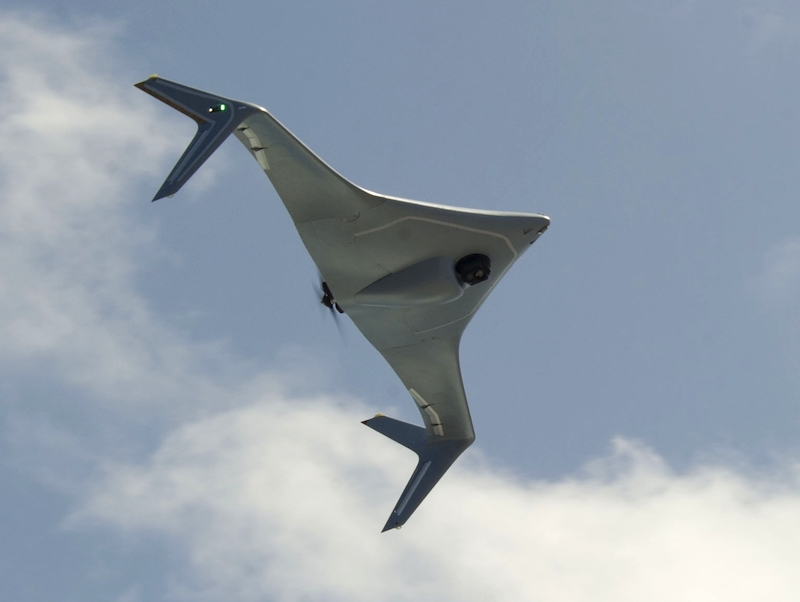
\includegraphics[width=.40\textwidth]{Northrop_Grumman_Bat_UAV_in_flight_in_June_2014.JPG}} \\
    \subfloat[][\emph{A DeltaQuad VTOL fixed wing surveillance UAV}.]{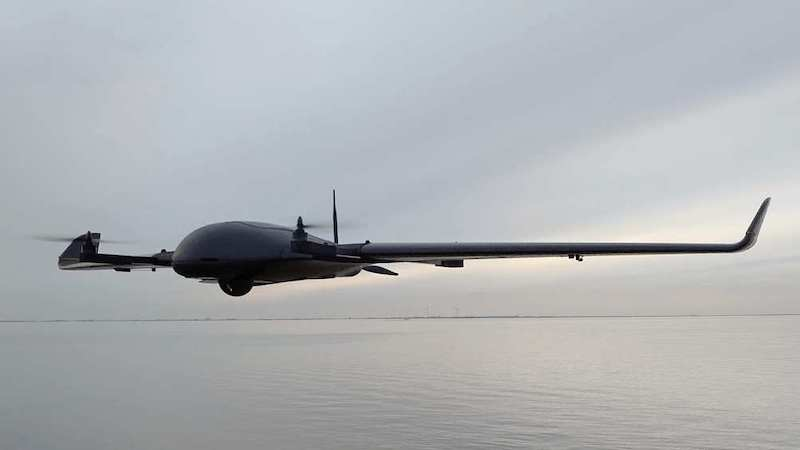
\includegraphics[width=.40\textwidth]{DeltaQuad_VTOL_surveillance_UAV.jpg}}
    \captionsource{UAVs used in various operations.}{
    \href{https://en.wikipedia.org/wiki/Unmanned_aerial_vehicle}{Wikipedia}}
    \label{fig:uavs-image}
\end{figure}
%
%
\subsection{UAV components}
\label{ssec:components}
%
Crewed and un-crewed aircraft of the same type generally have recognizably
similar physical components. One of the differences is the absence of the
cockpit and environmental control system or life support systems. Some UAVs
carry payloads such as a camera or other kinds sensors smaller and lightweight.
Small UAVs have assumed a characteristic quad-copter design particular
recognizable, although other scheme are realizable.
With the continuous development in the introduction of new parts or revisited 
ones the process of miniaturized require less-power propulsion and increase
battery runtime.\\
Control systems for UAVs are different for remote human control, a camera and
video link almost always replace the cockpit windows; radio-transmitted digital
commands replace physical cockpit controls. Autopilot software is used on both
crewed and uncrewed aircraft, with varying feature sets.\cite{wiki:uav}
%
%
\begin{figure}[htb]
    \centering
    \subfloat[][\emph{typical quadcopter design}.\label{subfig:quadcopter-design}]{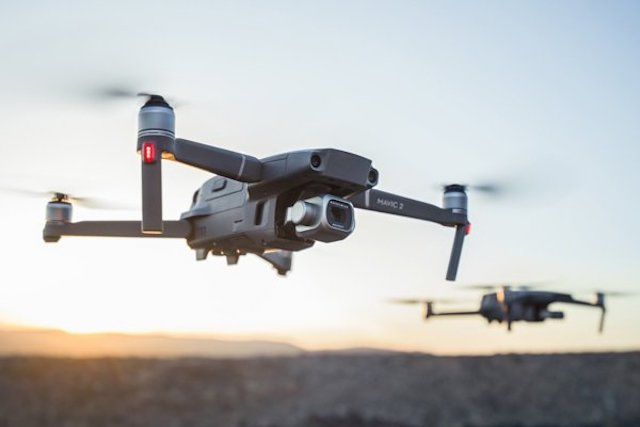
\includegraphics[width=.50\textwidth]{dji_mavic_2-1.jpg}} \quad
    \subfloat[][\emph{multirotor drone design}.\label{subfig:multicopter}]{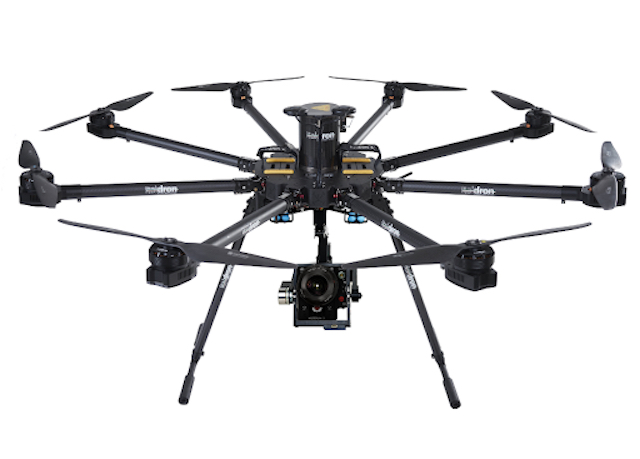
\includegraphics[width=.50\textwidth]{unnamed.jpg}}
    \captionsource{Example of design choices in the realization of UAVs shape}{
    \href{https://www.dji-store.it/guida-acquisto-migliori-droni-dji-per-riprese-aeree/}{DJI}; 
    \href{http://www.italdron.com/it/droni-professionali-e-accessori/droni-professionali/bigone-8hse-pro}{Italdron}}
    \label{fig:uav-design}
\end{figure}
%
%
\paragraph{Body} UAVs assume different configuration based on requirement of
task they perform for example aerial video shooting, surveys, territorial
control and many more.
Thus they are normally equipped with 4, 6, or 8 motor called quadcopter,
exacopter or octocopter.
The mainly difference that exist between different configuration is the payload
capacity that it can carry in flight.
%
\paragraph{Power supply}
Small UAVs mostly use lithium-polymer batteries (Li-Po), while larger vehicles
rely on conventional airplane engines. Scale or size of aircraft is not the
defining or limiting characteristic of energy supply for a UAV. 
Battery elimination circuitry (BEC) is used to centralize power distribution and
often harbors a microcontroller unit (MCU). Costlier switching BECs diminish
heating on the platform.\cite{wiki:uav}
%
\paragraph{Compuntig}
The hardware systems mounted on the drone have undergone an evolution in step
with the advancement of the IT sector, so much so that the analog controls have
been gradually replaced by microcontrollers up to System On Chip (SoC) with
single board cmaputer such as the Raspberry. In addition, UAVs are equipped with
flight controllers, flight controller boards and autopilots.
%
\paragraph{Sensors and Actuators}
Drone control is allowed through the cooperation of proprioceptive and
exteroceptive sensors that send their information to the central processing
unit.
The data coming from the platform measures accelerations and angular speeds
through accelerometers and gyroscopes that process and transmit the attitude
data such as orientation and position.
The GPS allows the spatial location of the aircraft on a map and to control the
route with respect to a planned trajectory. The altimeter allows you to
continuously record changes in altitude. The magnetometer is a device that
allows you to define the magnetic field vector at the point where you measure
with the drone and then obtain the orientation with respect to the North.
Knowledge and control of these measures allows the central system to allow
control of the actuators. Other more less common sensors may be present to
perform the most varied tasks.
%
\paragraph{Communications}
Most UAVs use a radio for remote control and exchange of video and other data.
The connections depending on the use cases and needs can be narrowband and
broadband. Generally, the sending and receiving of the commands is carried out
by means of a radio connection from the ground, especially for remote piloting.\\
Other connections that exploit protocols such as TCP/IP are used for sending
multimedia data such as filming areas and are transmitted to mobile devices such
as smartphones, tablets and so on.
Other types of connections can be used depending on the sector of use, in fact
for the military sector these may differ to ensure greater safety and
robustness.\\ 
More and more UAVs are implementing the MAVlink protocol for the
transport of data of control and control between piloting on the ground and
aircraft.
%
%
\subsection{Autonomy}
\label{ssec:autonomy}
%
UAVs have various levels of autonomy, that is, they are not completely
autonomous and do not require continuous intervention by the remote operator.
They have algorithms of return to the house which can be performed with a certain
level of autonomy. 
Up to high levels of autonomy which allow more complex operations. 
Autonomy derives from the awareness of the situation in which the drone is
located. 
The knowledge derives from the data acquired by the sensors mounted on board the
drone. 
The use of sensor fusion to integrate the information collected allows to limit
the error committed and to increase the precision and accuracy of the
information obtained. 
UAV's degrees of autonomy are often implemented by UAV manufacturers often build
in specific autonomous operations, such as:
\begin{itemize}
	\item Self-level: attitude stabilization on the pitch and roll axes.
	\item Altitude hold: The aircraft maintains its altitude using barometric or ground sensors.
	\item Hover/position hold: Keep level pitch and roll, stable yaw heading and altitude while maintaining position using GNSS or inertal sensors.
	\item Headless mode: Pitch control relative to the position of the pilot rather than relative to the vehicle's axes.
	\item Care-free: automatic roll and yaw control while moving horizontally.
	\item Take-off and landing (using a variety of aircraft or ground-based sensors and systems; see also:Autoland)
	\item Failsafe: automatic landing or return-to-home upon loss of control signal.
	\item Return-to-home: Fly back to the point of takeoff (often gaining altitude first to avoid possible intervening obstructions such as trees or buildings).
	\item Follow-me: Maintain relative position to a moving pilot or other object using GNSS, image recognition or homing beacon.
	\item GPS waypoint navigation: Using GNSS to navigate to an intermediate location on a travel path.
	\item Orbit around an object: Similar to Follow-me but continuously circle a target.
	\item Pre-programmed aerobatics (such as rolls and loops).\cite{wiki:uav}
\end{itemize}
%
%
\begin{figure}[htb]
	\centering
    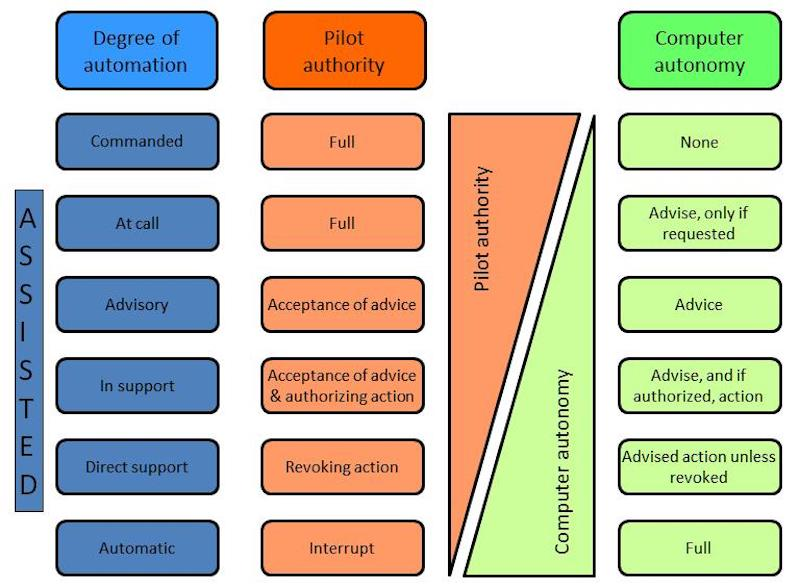
\includegraphics[width=0.50\textwidth]{Degrees_of_autonomy.jpg}
    \captionsource{UAV's degrees of autonomy.}{\href{https://en.wikipedia.org/wiki/Unmanned_aerial_vehicle}{Wikipedia}}
    \label{fig:uav-autonomy}
\end{figure}
%
    \chapter{Hardware}
\label{chap:hardware}
\lettrine[lines=3]{T}{his} chapter describes the hardware used to realize out
the project. Where the use of the Raspberry Pi single board computer designed to
have high performance both in education and science coupled with 8 mega-pixel
camera module CMOS sensor was an almost conditioned choice. Shows that
scientific and engineering--grade imagery can be produced with the Raspberry Pi
3 and its V2.1 camera module. It also presents a brief introduction to
thermography and its physical principles before introducing Lepton 2.5 thermal
camera module, made by the company FLIR which is currently one of the top
manufactures of thermal camera solutions. The Coral Dev Board is a single-board
computer that contains an Edge TPU coprocessor. It's ideal for prototyping new
projects that demand fast on-device inferencing for machine learning models. The
Coral Dev Board is ideal when you need to perform fast machine learning (ML)
inferencing in a small form factor.
%
\section{Raspberry Pi 3}
\label{sec:raspi3}
The Raspberry Pi is a high-performance single-board computer designed to
experiment and solve real-world problems. This small computer supports a camera
module that uses a Sony IMX219 8 mega-pixel CMOS sensor.
%
\subsection{Specification}
\label{ssec:raspispecification}
As of early 2016, over 8 million Raspberry Pi's had been sold, making it one of
the most popular single-board computers on the
market.\cite{upton2016raspberry}\\ The Raspberry Pi credit-card-sized computer
supports several accessories, including a camera module containing the Sony
IMX219 sensor. This computer and camera configuration is of particular interest
since it can provide raw-data format imagery that can be used for a multitude of
applications, including computer vision, biophotonics, medical testing, remote
sensing, astronomy, improved image quality, high dynamic range (HDR) imaging,
and security monitoring. The Raspberry Pi 3 is the third generation single board
Raspberry Pi computer and became available to consumers in February 2016. \\Some
of the more significant Raspberry Pi attributes, including interfaces, are
described in Table \ref{tab:rapberryattributes}. The Raspberry
Pi Foundation provides several operating systems for the  Raspberry Pi 3,
including Raspbian and a Debian-based Linux distribution, as  well as
third-party Ubuntu, Windows 10 IOT Core, RISC OS, and specialized  distributions
for download.\cite{10.1117/1.JEI.26.1.013014}
%
\begin{table}[htb]
\centering
	\caption{Raspberry Pi 3 computer attributes.}
	\label{tab:rapberryattributes}
	\begin{tabular}{l}
		\hline
		CPU 1.2 \si{\giga\hertz} 64-bit ARM Cortex-A53 \\
		1 GB of RAM LPDDR2 (900 \si{\mega\hertz}) \\
		Wireless N and Blue-tooth 4.1 communication\\
		Four USB ports\\
		HDMI interface\\
		Ethernet port\\
		MicroSD card slot\\
		40 GPIO pins\\
		Camera interface\\
		Composite video audio jack\\
		\hline
\end{tabular}
\end{table}
%
\section{Raspberry Pi, Camera Board V2}
\label{sec:raspicam}
The camera is based on the Sony IMX219 silicon CMOS back-lit sensor and produces
8 mega-pixel images that are $3280 \times 2464$ pixels in size. \\
The IMX219 sensor operates in the visible spectral range from 400 to 700 \si{\nano\meter}).\cite{raspberrycam2}
Sensor specifications are detailed in Table \ref{tab:raspicamspec}.
%
\begin{table}[!h]
	\centering
	\caption{Sony IMX219 sensor chip specifications.}
	\label{tab:raspicamspec}
	\begin{tabular}{l l}
		\hline
		\textbf{Sensor parameter}			& 	\textbf{Specification}\\
		\hline
		Image sensor type		&	Back-lit CMOS\\
		Image size				&	Diagonal 4.60 \si{\milli\meter} (type 1/4.0)\\
		Number of active pixels	&	3280 (H) $\times$ 2464 (V) $\sim$ 8.08 mega-pixels\\
		Chip size				&	5.095 \si{\milli\meter} (H) $\times$ 4.930 \si{\milli\meter}(V) (w/ Scribe)\\	
		Unit cell size (pixel) 	&	1.12 \si{\micro\meter} (H) $\times$ 1.12 \si{\micro\meter}(V)\\
		Substrate material		&	Silicon\\
		Bit depth				&	10-bit A/D converter on chip\\
		Data output				&	CSI2 serial data output (selection of 4 lane/ 2 lane)\\
		Communication			&	2-wire serial communication circuit on chip\\
		Max full-frame frame rate &	30 frames/s \\
		Pixel rate 				&	280 mega-pixel/s (all-pixels mode)\\
		Data rate				&	Max. 755 Mbps/lane (at 4 lane), 912 Mbps / lane(at 2 lane)\\
		\hline
	\end{tabular}
\end{table}
%
\subsection{Specification}
\label{ssec:raspcamspecification}
The V2 camera module operates at a fixed focal length (3.04 \si{\milli\meter})
and single $f$-number (F$2.0$) typically focused from the near-field to
infinity. Images can be captured at ISO settings between 100 and 800 in manually
set increments of 100
and camera exposure times between \SI{9}{\micro\second} and 6 \si{\second} using
a rolling shutter. Some of the more significant camera specifications are shown
in Table \ref{tab:raspicamspec2}. In addition to still photos, the Raspberry Pi
Sony IMX219 sensor supports a cropped 1080p format at 30 frames per second (fps)
and full-frame imaging video at up to 15 fps, but not in raw-data format. The
entire camera board is small 25 \si{\milli\meter} $\times$ 25 \si{\milli\meter}
$\times$ 9 \si{\milli\meter} and weighing about $3$ \si{\gram}. It connects
directly to the Raspberry Pi 3 through a 15 pin mobile industry processor
interface (MIPI) camera serial interface and is shown alongside a Raspberry Pi 3
in Figure \ref{fig:boardcam}.\cite{upton2016raspberry, raspberrycam}
%
\begin{table}[htb]
	\centering
	\caption{Raspberry Pi camera.}
	\label{tab:raspicamspec2}
	\begin{tabular}{l l}
		\hline
		\textbf{Camera parameter}			& 	\textbf{Specification}\\
		\hline
		Lens focal length 	& 	3.04 \si{\milli\meter}	\\
		$f$-number			&	2.0	\\
		Instantaneous field of view	&	0.368 \si{\milli\radian}\\
		Full-frame field of view & 59.17 \si{\degree}(H) $\times$ 58.3 \si{\degree} (V)\\
		\hline
	\end{tabular}
\end{table}
%

\begin{figure}[htb]
	\centering
    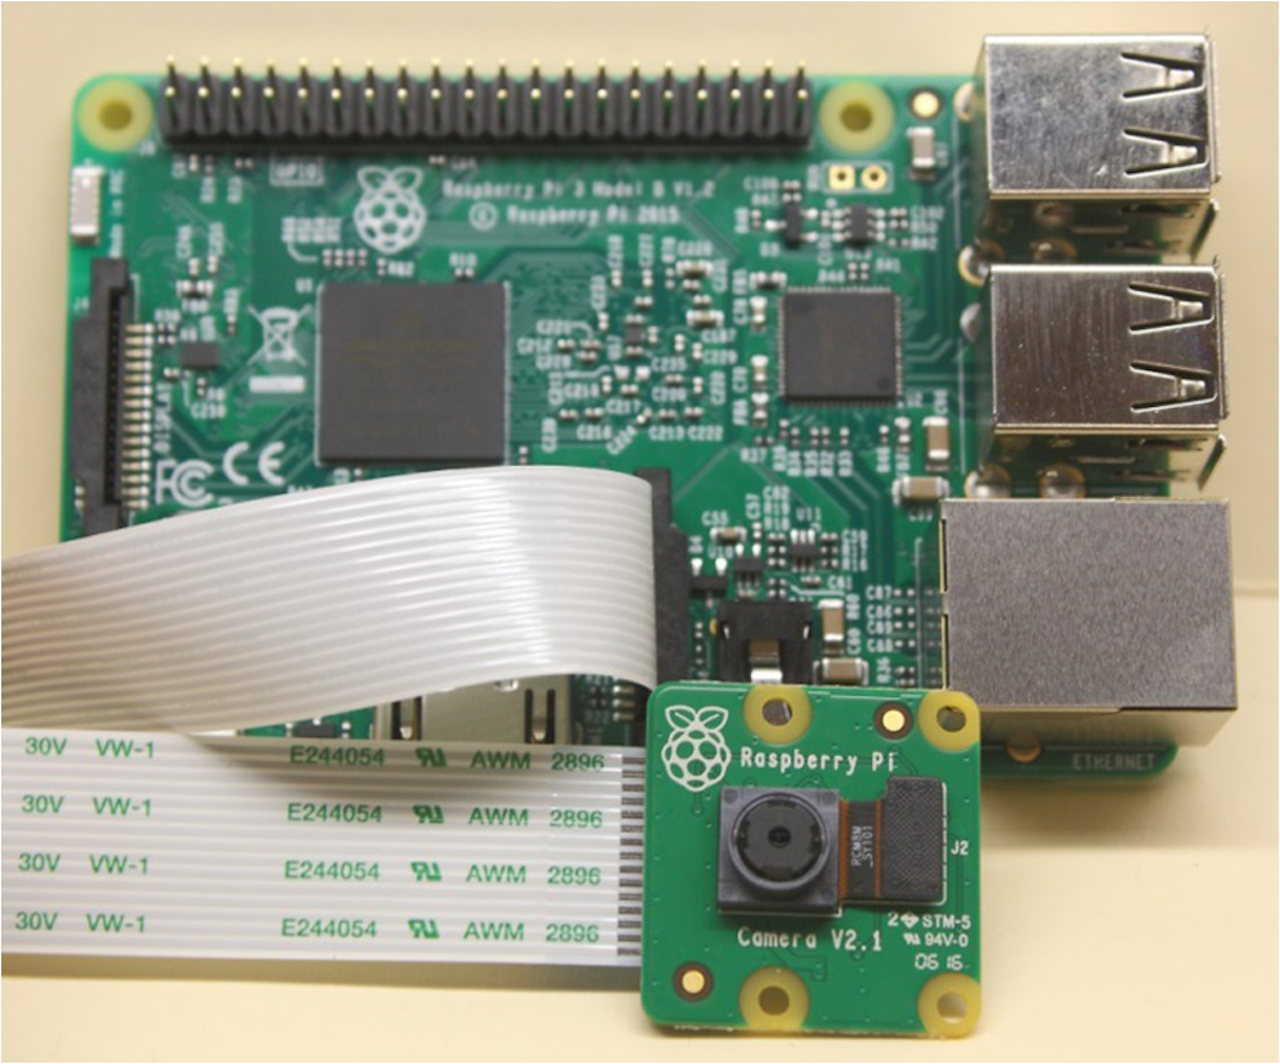
\includegraphics[width=0.80\textwidth]{JEI_26_1_013014_f001.png}
    \caption{Raspberry Pi 3 and camera module V2.1.}
    \label{fig:boardcam}
\end{figure}
\section{Thermal imaging theory}
\label{sec:theory}
The story of infra-red imaging started in 1800, when Herschel discovered 
infra-red radiation experimentally at long wavelengths just outside the visible 
spectrum of sun light.
The quantitative explanation of incandescent infra-red radiation in 1900 by Max 
Planck started a development, which today has resulted in modern infra-red 
technologies with infra-red camera systems These are also the result of 
scientific developments in semiconductor physics and micro-system 
technologies.\cite{10.1117/12.2266142}
Since its birth, it is possible to recognize three generations of infra-red 
cameras\cite{thermalimage}: the first generation cameras were characterized by 
a single element detector, combined with two scanning mirrors to create 
infra-red images. 
Their main disadvantage was that they suffered from saturation problems. 
Saturation indicates the limit of the highest irradiation that can be measured 
by a detector. For digital sensors, since incident photoelectrons are converted 
in charges, each detector can store a maximum amount of charges known as the 
full well capacity.\cite{10.1117/12.2266142}
The second generation cameras were characterized by an increase in the number 
of detectors, positioned in a large linear array or in two small 2-D array.
The third generation cameras, i.e., the ones currently used, are characterized 
by large focal plane array (FPA) detectors, thus increasing the reliability 
and sensitivity of such infra-red systems.\cite{rogalski2000infrared} 
%
\subsection{Electromagnetic radiation}
\label{ssec:electromagnetic-radiation}
Electromagnetic radiation is all around (and within, and throughout) us and is
comprised of everything from gamma radiation on the high frequency end to radio
waves on the low frequency end. So the Figure (\ref{fig:spectrum}) give an
overview of EM waves, ordered according to their wave-length or frequency. 
This spectrum consists of a great variety of different waves. All of them can
be observed in nature, and many have technical applications. Starting from the
left of the figure, for example, $\gamma$-rays have the highest frequencies,
that is, the shortest wavelengths.\cite{vollmer2017infrared} \hfill \break
%
%
\begin{figure}[htb]
	\centering
	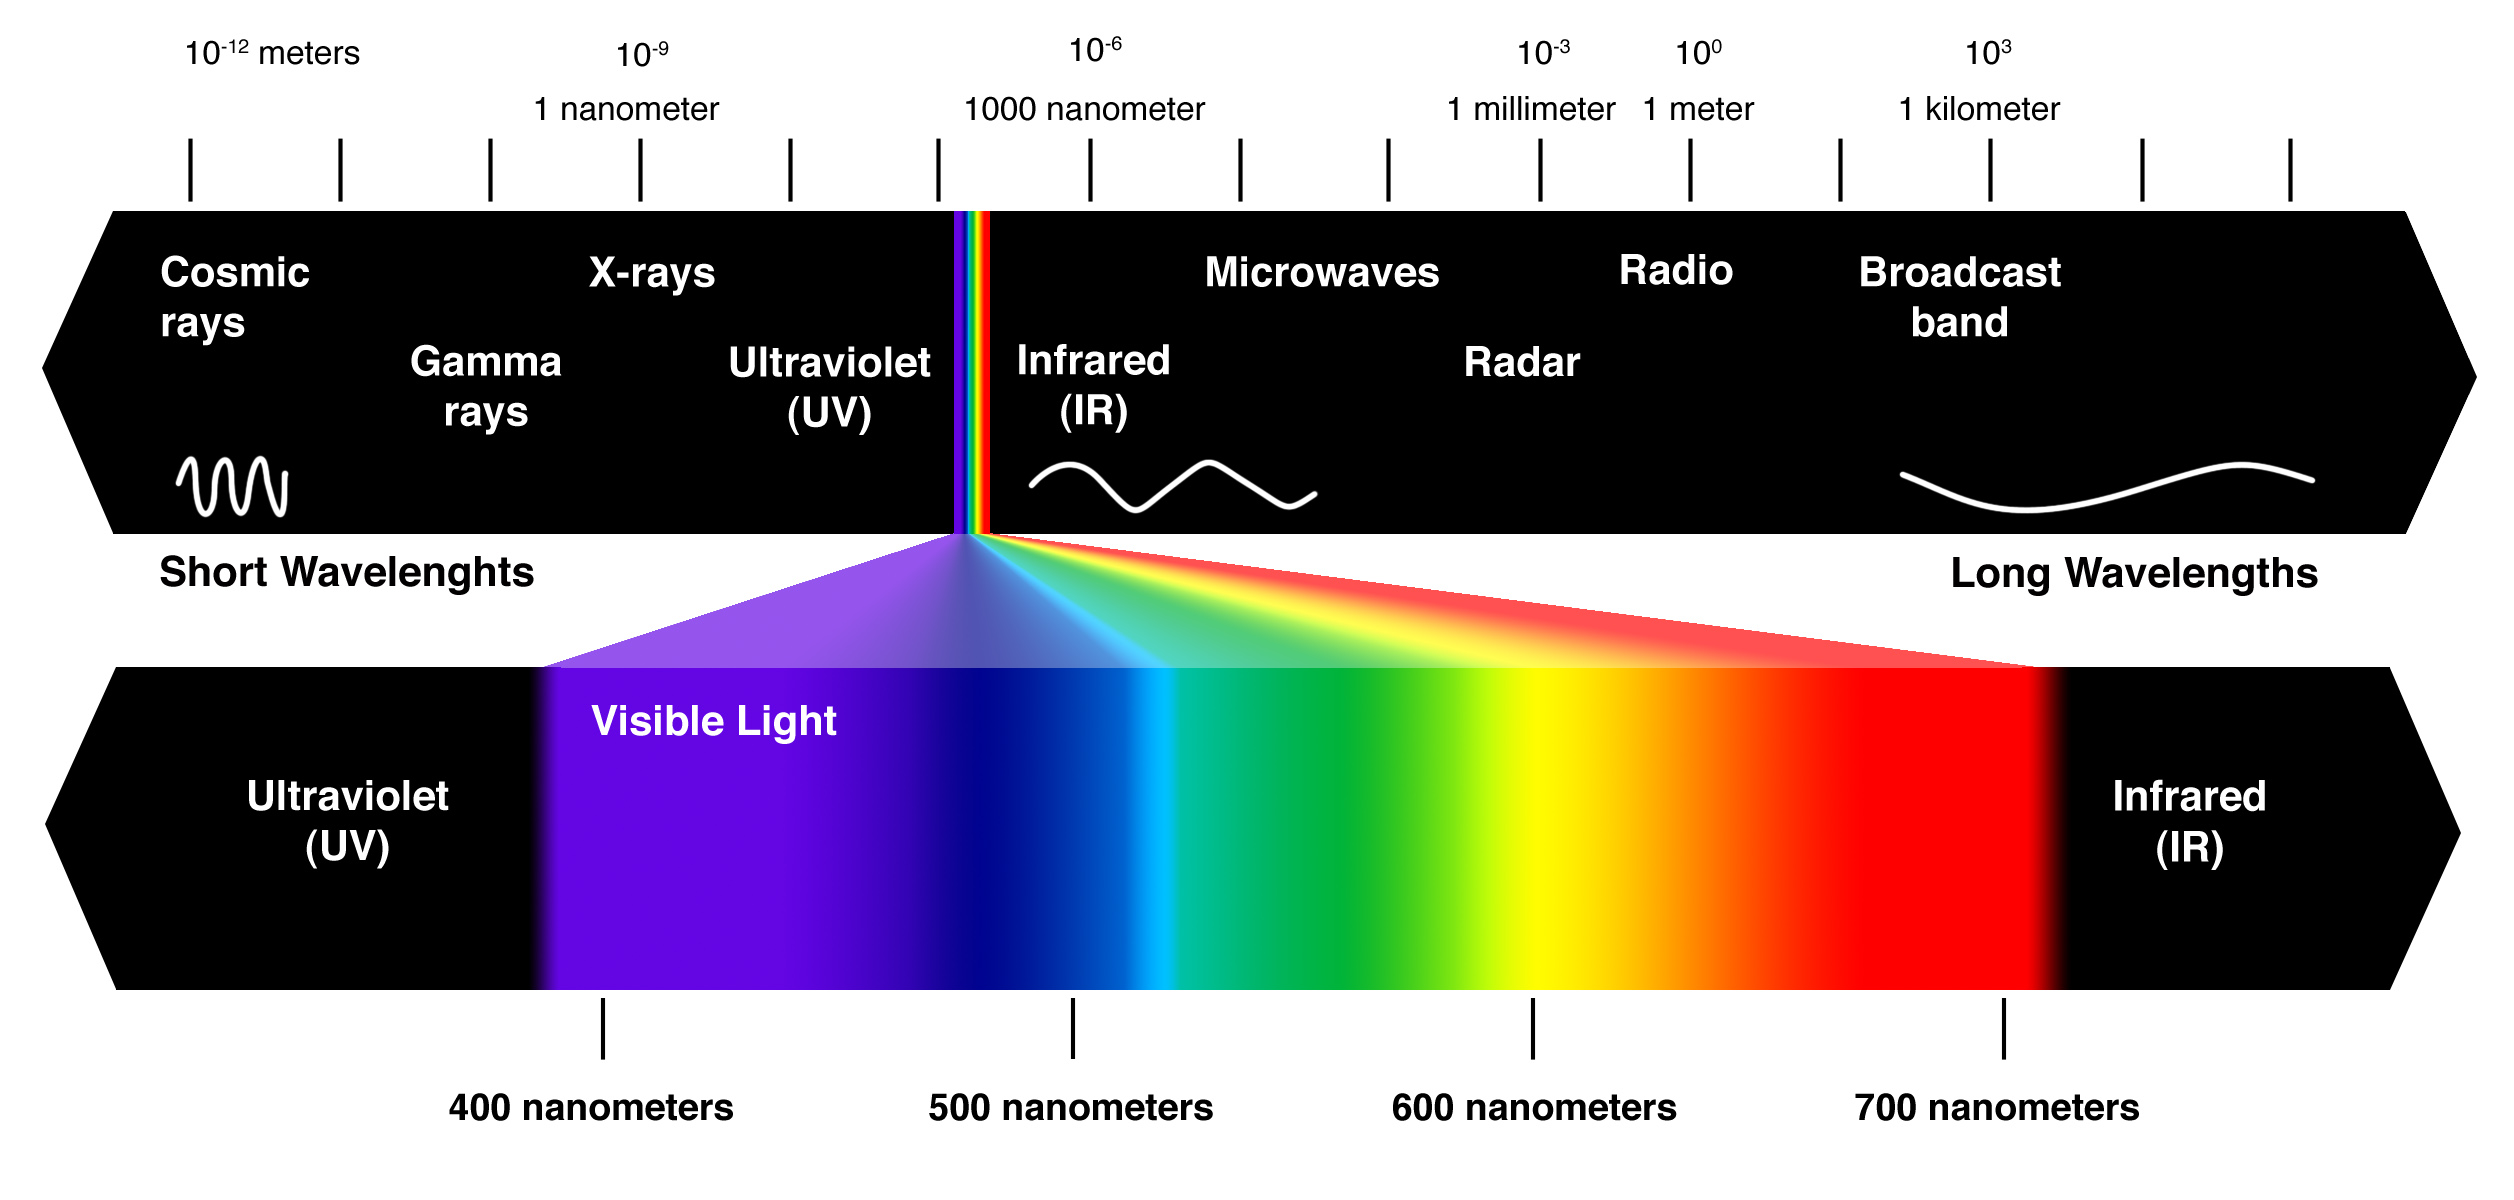
\includegraphics[width=0.65\textwidth]{Visible-spectrum.jpeg}
	\captionsource{Composition of the spectrum of electromagnetic waves.}{
	\href{https://socratic.org/questions/what-is-the-wavelength-of-a-photon-of-blue-light-whose-frequency-is-6-3-10-14-s-}{https://socratic.org}}
	\label{fig:spectrum}
\end{figure}
%
\newline
The visible light, defined by the sensitive range of the light receptors in our
eyes, only covers a very small range within this spectrum, with wavelengths from
$380$ to $780$ \si{\nano\meter}. The adjacent spectral region with wavelengths
from $780$ \si{\nano\meter} up to $1$ \si{\milli\meter} is usually called infra-red. 
This range is followed by microwaves, RADAR, and all EM waves that are used for
radio, TV, and so on.
While most imaging sensors detect radiation in the visible spectrum (wavelengths
from $380$ to $700 \,\si{\nano\meter}$), long wave infra-red sensors detect
radiation the infra-red spectrum, and it accounts for most of the thermal
radiation emitted by objects near room temperature. Then for IR imaging, only a
small range of the IR spectrum is used. It is shown in an expanded view in
Figure (\ref{fig:spectrum-ir}). Typically, three spectral ranges are defined for thermography: 
the long-wave (LW) region from around $8$ to $14$ \si{\micro\meter}, the
mid-wave (MW) region from around $3$ to $5$ \si{\micro\meter}, and the 
short-wave (SW) region from $0.9$ to $1.7$ \si{\micro\meter}.
%
%
\begin{figure}[!h]
	\centering
	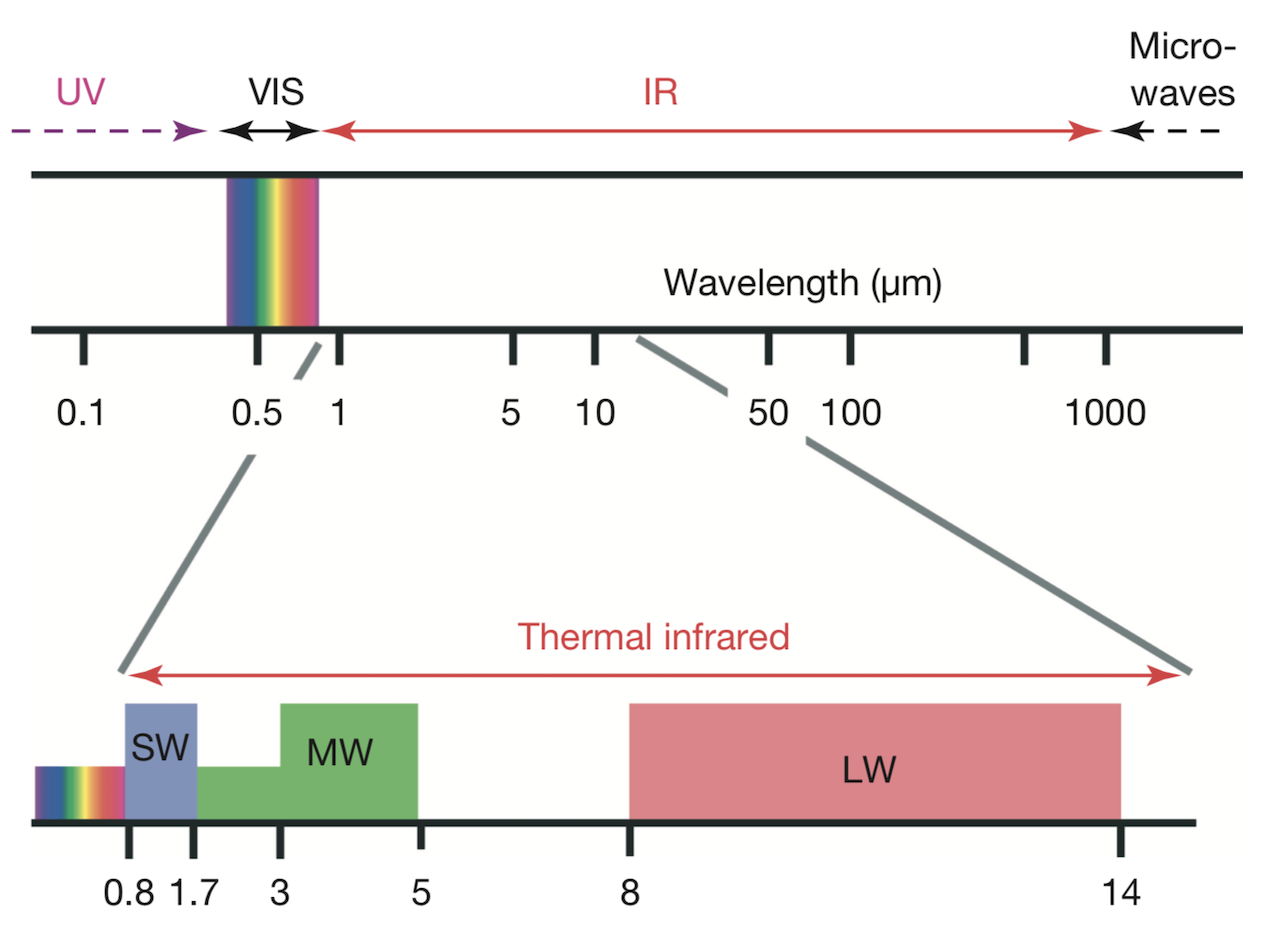
\includegraphics[width=0.65\textwidth]{spectrum-ir.png}
	\captionsource{Infrared (IR) and adjacent spectral regions and expanded view of so-called thermal IR. This is the region where IR imaging systems for short-wave (SW), mid-wave (MW), and long- wave (LW) cameras exist. Special systems have extended ranges.
}{\cite{vollmer2017infrared}}
	\label{fig:spectrum-ir}
\end{figure}
% 
The origin of naturally occurring EM radiation is manifold. 
The most important phenom for thermography is the thermal radiation. 
In brief, the thermal radiation implies that every body or object at a
temperature T $>0 \,$ \si{\kelvin} $\,(-273.15 \,$\si{\celsius}$)$ emits EM
radiation. 
The amount of radiation and its distribution as a function of wavelength depend
on temperature and material properties. \cite{vollmer2017infrared} 
For temperatures in the range of natural and technological processes, this 
radiation is in the thermal IR spectral region. 
This is known as the infra-red spectrum, and it accounts for most of the
thermal radiation emitted by objects near room temperature.
%
\subsection{Modern detectors}
\label{ssec:modern-detect}
The main difference between a thermal imaging and normal image capturing is the
sensor used. One type of the sensor used in thermal cameras is called a
microbolometer. Essentially its functionality is similar to the CMOS or CCD
sensor, just in different wavelengths. Unlike many other thermal sensor the
microbolometer doesn't need an active cooling system to function a long period
of times. Modern uncooled detectors use sensors whose working mechanism is based
on a change of resistance, voltage or current when heated by IR radiation.
Uncooled detectors are mostly composed by pyroelectric and ferroelectric
materials or based on microbolometer technology. The thermal signal depends upon
the radiant power but not upon its spectral content, i.e., it is wavelength
independent.\cite{10.1117/12.2266142,rogalski2000infrared}

\section{Thermal Camera module Lepton 2.5}
\label{sec:thermalcamera}
The thermal camera module we use in this project, we will go through its
specification, modes of capture and communication protocol for both video frame
transfer and camera control. Information about the camera are extracted from
official documentation.

% TODO CHECK DOCUMENTATION AND LINK IN REFERENCE-BIBLIOGRAPHY

% TODO INSERT IMAGE FLIR LEPTON

\subsection{Specification}
\label{ssec:specificationthermalcam}
Lepton is an infra-red camera system that integrates a fixed-focus lens assembly,
an $80 \times 60$ long-wave infra-red (LWIR) micro-bolometer sensor array, and
signal-processing electronics. Easy to integrate and operate, Lepton is intended
for mobile devices as well as any other application requiring very small
footprint, very low power, and instant-on operation. Lepton can be operated in
its default mode or configured into other modes through a command and control
interface (CCI). The effective frame rate of the camera is only 8.6 \si{\hertz},
however for our needs this is not a problem. The camera only requires low
voltage supply and has small power consumption of around 140 \si{\milli\watt}.
%
\begin{table}[htb]
    \centering
    \caption{Key Specifications}
    \label{tab:thcamspecifications}
    \begin{tabular}{l c c}
        \hline
                                                            &   FLIR Lepton 2.5 	&          	\\
        \hline
        \rowcolor{aliceblue!85} Resolution (h x w)	       	&   80 $\times$ 60  	&	pixels	\\
        Spectral Range	                                    	&   8  to 14        	&	\si{\micro\meter}	\\
        \rowcolor{aliceblue!85} Horizontal Field of View		&   51              	&   \si{\degree}			\\
        Thermal Sensitivity	                                	&   < 50            	&   \si{\milli\kelvin}	\\
        \rowcolor{aliceblue!85} Frame Rate	                	&   < 9             	&   \si{\hertz} 			\\
        Control Interface	                                	&   I$^{2}$C        	&               			\\
        \rowcolor{aliceblue!85} Video Interface	            	&   SPI             	&               			\\
        Promised Time to Image	                            	&   < 0.5           	&   \si{\second}    		\\
        \rowcolor{aliceblue!85} Integral Shutter		    		&   yes             	&   			\\
        Radiometry	                                        	&   14-bit pixel value  	&       \\
        \rowcolor{aliceblue!85} Operating Power             	&	$\sim$150       	&   \si{\milli\watt} 	\\
        \hline
\end{tabular}
\end{table}
%
See table \ref{tab:thcamspecifications} for more specifications.\\For better
manipulation with the camera module we use a breakout board (figure 3.1) with a
housing for the Lepton camera module. The breakout board provides better
physical accessibility, improves heat dissipation and increases input voltage
supply range to 3--5 \si{\volt}, as it has its own regulated power supply. This
power supply provides the camera module with three necessary voltages: 1.2, 2.8
and 2.5--3.1 \si{\volt}. The breakout board also supplies the camera with master
clock signal. [14] \\
The camera uses two interfaces for communication:
\begin{itemize}
    \item SPI for transferring video frames from the camera to a SPI master
device.
    \item I$^{2}$C for receiving control commands from the I$^{2}$C master
device.
\end{itemize}
Even though the name of the project include the keyword low-cost, we need to
think of this statement with respect to the thermal camera market. The Lepton 3
thermal camera module can be considered low-cost when compared to other thermal
camera devices available as it costs around $250$ (2018) 4. This could however
be considerably more when compared to other nonthermal solutions, however way
more than if we would utilize a simple infra-red counting sensors for example.
%
\begin{figure}[htb]
    \centering
    \resizebox{0.8\textwidth}{!}{\begin{tikzpicture}
    \draw[help lines] (0,0) grid (20, 20);
%     \draw (0,0) rectangle (10,20);
% \draw[fill=cyan!50] (1,1) rectangle (7,3)   node {Camera Supply Inputs};
% \draw[fill=cyan!50] (1,3) rectangle (7,6)   node {Camera Shut Down};
% \draw[fill=cyan] (1,6) rectangle (7,11) node {Camera Reset};
% \draw[fill=cyan!50] (1,11) rectangle (7,13) node {Camera Clock Gneration};
% \draw[fill=cyan!50] (1,13) rectangle (7,15) node {Camera };
% \draw[fill=cyan!50] (1,15) rectangle (7,17) node {Camera };
% \draw[fill=cyan!50] (1,17) rectangle (7,19) node {Camera };
% \draw[fill=cyan!50] (1,1) rectangle (,);
% \draw[fill=cyan!50] (1,1) rectangle (,);
% \draw[fill=cyan!50] (1,1) rectangle (,);
% \draw[fill=cyan!50] (1,1) rectangle (,);
% \draw[fill=cyan!50] (1,1) rectangle (,);
% \draw[fill=cyan!50] (1,1) rectangle (,);
% \draw[fill=cyan!50] (1,1) rectangle (,);
% \draw[fill=cyan!50] (1,1) rectangle (,);
% \draw[fill=cyan!50] (1,1) rectangle (,);
% \draw[fill=cyan!50] (1,1) rectangle (,);
% \draw[fill=cyan!50] (1,1) rectangle (,);
% \draw[fill=cyan!50] (1,1) rectangle (,);
% \draw[fill=cyan!50] (1,1) rectangle (,);
% \draw[fill=cyan!50] (1,1) rectangle (,);
% \draw[fill=cyan!50] (1,1) rectangle (,);








\end{tikzpicture}
}
    \caption{my figure drawn in tikz}\label{fig:myfigure}
\end{figure}
%
\subsection{System Architecture}
\label{ssec:leptonarchitecture}
The lens assembly focuses infrared radiation from the scene onto an $80 \times 60$ array
of thermal detectors with 17-micron pitch. Each detector element is a
vanadium-oxide (VOx) microbolometer whose temperature fluctuates in response to
incident flux. The change in temperature causes a proportional change in each
microbolometer’s resistance. VOx provides a high temperature coefficient of
resistance (TCR) and low 1/f noise, resulting in excellent thermal sensitivity
and stable uniformity. The microbolometer array is grown monolithically on top
of a readout integrated circuit (ROIC) to comprise the complete focal plane
array (FPA). Once per frame, the ROIC senses the resistance of each detector by
applying a bias voltage and integrating the resulting current for a finite
period of time called the integration period. The serial stream from the FPA is
received by a system on a chip (SoC) device, which provides signal processing
and output formatting.
%
\begin{figure}[htb]
    \centering
    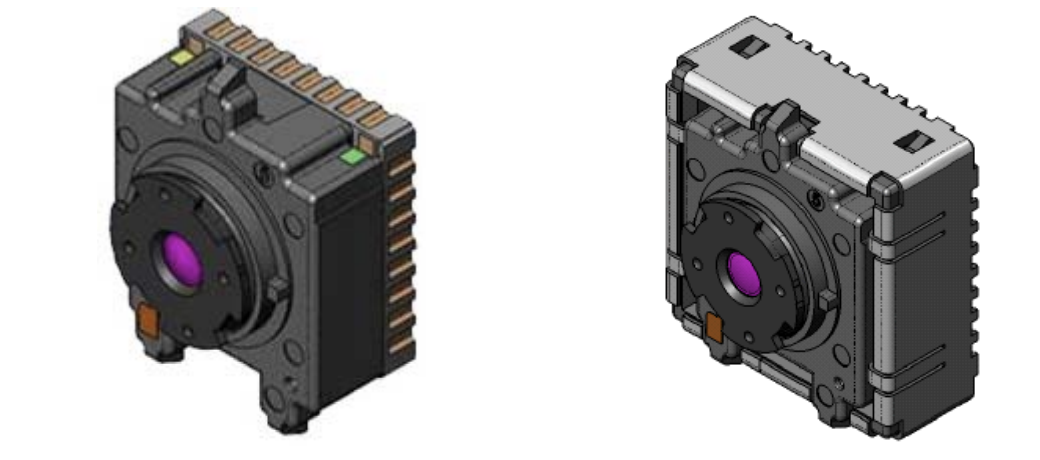
\includegraphics[width=0.80\textwidth]{leptoncamera.png}
    \caption{Lepton Camera (with and without socket)}
    \label{fig:camerarender}
\end{figure}
%
\subsection{video pipeline}
\label{ssec:pipeline}
The video pipeline includes non-uniformity correction (NUC), defect replacement,
spatial and temporal filtering, automatic gain correction (AGC), and
colourization.
%
%insert image video stream
%
% nuc
\paragraph{The non-uniformity correction (NUC)} block applies correction
terms to ensure that the camera produces a uniform output for each pixel when
imaging a uniform thermal scene. Factory-calibrated terms are applied to
compensate for temperature effects, pixel response variations, and
lens-illumination roll-off. To compensate for temporal drift, the NUC block also
applies an offset term that can be periodically updated at runtime via a process
called flat-field correction (FFC). The FFC process is further described in FFC
States, (\ref{ssec:FFCstates}).
%
%7.2 Defect Replacement
\paragraph{The defect-replacement} block substitutes for any pixels identified
as defective during factory calibration or during runtime. The replacement
algorithm assesses the values of neighboring pixels and calculates an optimum
replacement value. The typical number of defective pixels is $\leq 1$.
%
\paragraph{Temporal Filtering} the image pipeline includes a number of
sophisticated image filters designed to enhance signal-to-noise ratio (SNR) by
eliminating temporal noise and residual non-uniformity. The filtering suite
includes a scene-based non-uniformity correction (SBNUC) algorithm which relies
on motion within the scene to isolate fixed pattern noise (FPN) from image
content.
%
\paragraph{The AGC algorithm} for converting the full-resolution (14-bit)
thermal image into a contrast-enhanced image suitable for display is a
histogram-based non-linear mapping function. See (\ref{ssec:AGCModes}).
%
\paragraph{The colorize block} takes the contrast-enhanced thermal image as
input and generates a 24-bit RGB color output.
%
\subsection{Power States}
\label{ssec:powerstate}
Lepton currently provides five power states. As depicted in the state diagram
shown in Figure 6, most of the transitions among the power states are the result
of explicit action from the host. The automatic transition to and from the
overtemp state is an exception. In the figure, transitions that require specific
host-side action are shown in bold. Automatic transitions are not bolded.
%
\begin{itemize}
    \item Off: When no voltage is applied, Lepton is in the off
state. In the off state, no camera functions are available.
    \item Uninitialized:
In the uninitialized state, all voltage forms are applied, but Lepton has not
yet been booted and is in an indeterminate state. It is not recommended to leave
Lepton in this state as power is not optimized; it should instead be booted to
the on-state (and then transitioned back to standby if imaging is not required).
    \item On: In the on state, all functions and interfaces are fully available.
    \item Standby: In the standby state, all voltage forms are applied, but power
consumption is approximately 4 \si{\milli\watt}. In the standby state, no
functions are available, but it is possible to transition to the on state via
the start-up sequence defined in Figure 7 on page 16. The shutdown sequence
shown in Figure 7 on page 16 is the recommended transition back to the standby
state. It is also possible to transition between standby and on states via
software commands, as further defined in the software IDD.
    \item Overtemp: The
overtemp state is automatically entered when the Lepton senses that its
temperature has exceeded approximately $80$ \si{\celsius}. Upon entering the
overtemp state, Lepton enables a ``\emph{shutdown imminent}" status bit in the
telemetry line and starts a $10$ \si{\second} counter. If the temperature of the
Lepton falls below $80$ \si{\celsius} before the counter times out, the
``\emph{shutdown imminent}" bit is cleared and the system transitions back to
the on state. If the counter does time out, Lepton automatically transitions to
the standby state.
\end{itemize}
%
\subsection{FFC States}
\label{ssec:FFCstates}
Lepton is factory calibrated to produce an output image that is highly uniform,
such as shown in Figure \ref{subfig:Highly uniform image}, when viewing a
uniform-temperature scene. However, drift effects over long periods of time
degrade uniformity, resulting in imagery which appears more grainy (Figure
\ref{subfig:Grainy image}) and/or blotchy (Figure \ref{subfig:Blotchy image}).
Operation over a wide temperature range (for example, powering on at $-10$
\si{\celsius} and heating to $65$ \si{\celsius}) will also have a detrimental
effect on image quality. For scenarios in which there is ample scene movement,
such as most handheld applications, Lepton is capable of automatically
compensating for drift effects using an internal algorithm called scene-based
non-uniformity correction (scene-based NUC or SBNUC). However, for use cases in
which the scene is essentially stationary, such as fixed-mount applications,
scene-based NUC is less effective. In those applications, it is recommended to
periodically perform a flat-field correction (FFC). FFC is a process whereby the
NUC terms applied by the camera's signal processing engine are automatically
recalibrated to produce the most optimal image quality. The sensor is briefly
exposed to a uniform thermal scene, and the camera updates the NUC terms to
ensure uniform output. The entire FFC process takes less than a second.
%
\begin{figure}[htb]
    \centering
    \subfloat[][\emph{Highly uniform image}.\label{subfig:Highly uniform image}]
        {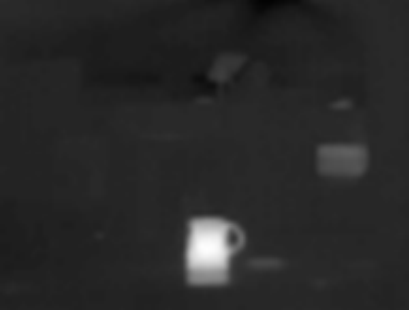
\includegraphics[width=.30\textwidth]{linearAGCa}} \quad
    \subfloat[][\emph{Grainy image
    (high-spatial frequency noise)}.\label{subfig:Grainy image}]
        {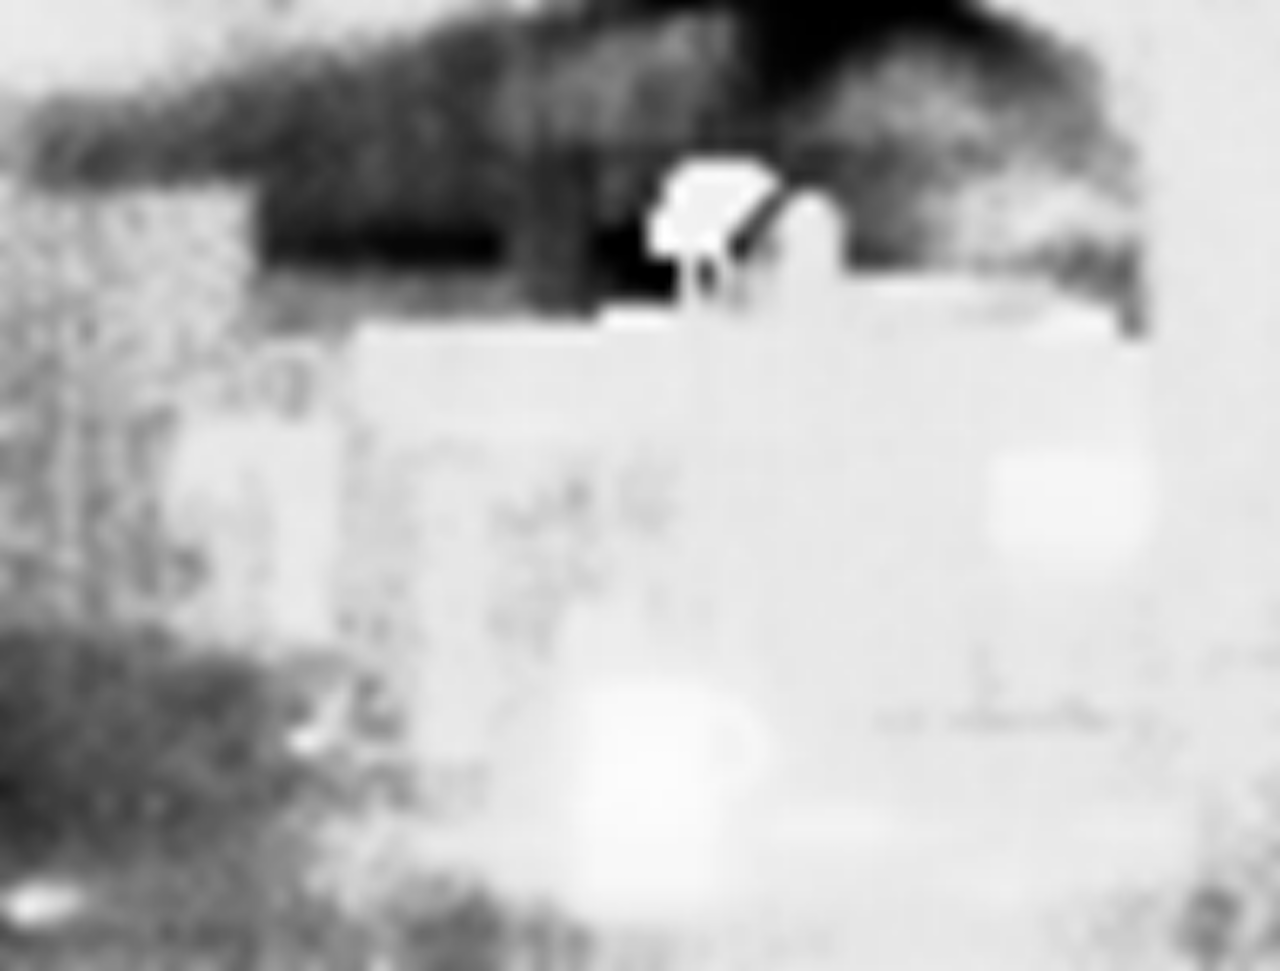
\includegraphics[width=.30\textwidth]{linearAGCb.png}} \quad
    \subfloat[][\emph{ Blotchy image
    (low-spatial frequency noise)}.\label{subfig:Blotchy image}]
        {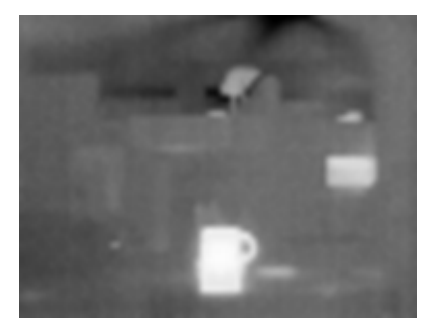
\includegraphics[width=.30\textwidth]{linearAGCc.png}}
    \caption{Examples of Good Uniformity, Graininess, and Blotchiness}
    \label{fig:exampleffc}
\end{figure}
%
\\The current FFC state is provided through the telemetry line. There are three
FFC states, as illustrated in Figure \ref{fig:FFC States}:
\begin{enumerate}
    \item FFC not commanded (default): In this state, Lepton applies by default a
set of factory-generated FFC terms.
    \item FFC in progress: Lepton enters this
state when FFC is commanded. The default FFC duration is nominally $23$ frames.
    \item FFC complete: Lepton automatically enters this state whenever FFC is
completed. Lepton also provides an ``FFC desired" flag in the telemetry line.
The ``FFC desired" flag is asserted at start-up, when a specified period
(default = 3 minutes) has elapsed since the last FFC, or when the sensor
temperature has changed by a specified value (default = 3 \si{\celsius}) since
the last FFC. The ``FFC desired" flag is intended to indicate to the host to
command an FFC at the next possible opportunity.
\end{enumerate}
%
\begin{figure}[htb]
    \centering
    \resizebox{0.35\textwidth}{!}{\begin{tikzpicture}
    \node (start) at (1,12) {Lepton powered on};
    \node [ellipse, fill=babyblueeyes, align=center] (notcommand) at (1,10) {FFC Not \\ Commanded};
    \node [ellipse, fill=babyblueeyes] (progress) at (1,8) {FFC In Progress};
    \node [ellipse, fill=babyblueeyes] (complete) at (1,6) {FFC Complete};
    \draw [-latex] (start) to (notcommand);
    % connections
    \path[-latex] (notcommand)  edge [bend right=50]    node[left] {\tiny{FFC Commanded}} (progress);
    \path[-latex] (progress)    edge [bend left=50]     node[right] {\tiny{FFC Complete}} (complete);
    \path[-latex] (complete)    edge [bend left=50]     node[left] {\tiny{FFC Commanded}} (progress);
\end{tikzpicture}
}
    \caption{FFC States.}
    \label{fig:FFC States}
\end{figure}
%
\subsection{AGC Modes}
\label{ssec:AGCModes}
There are two AGC modes:
\begin{itemize}
    \item AGC disabled (default)
    \item AGC enabled
\end{itemize}
AGC is a process whereby the large dynamic range of the infrared sensor is
collapsed to a range more appropriate for a display system. For Lepton, this is
a 14-bit to 8-bit conversion. In its most simplistic form, AGC can be a linear
mapping from 14-bit to 8-bit; however, a simple linear AGC is generally
incapable of providing pleasing imagery in all imaging conditions. For example,
when a scene includes both cold and hot regions (for example, a hot object in
front of a cold background as illustrated in \ref{fig:comparisionlinearAGC},
linear AGC can produce an output image in which most pixels are mapped to either
full black or full white with very little use of the gray shades (8-bit values)
in between. Because of this limitation of linear AGC, a more sophisticated
algorithm is preferred. Similar to most AGC algorithms that optimize the use of
gray shades, Lepton's is histogram-based. Essentially a histogram counts the
number of pixels in each frame that have a given 14-bit value. Figure
\ref{fig:histogram} the concept for a 3x3 pixel area.\linebreak
%
\begin{figure}[!h]
    \centering
    \resizebox{0.80\textwidth}{!}{\begin{tikzpicture}
    \begin{scope}[xshift=-35mm]
        % upper row
        \node [rectangle, minimum size=15mm, fill={rgb,255:red,170; green,170; blue,170}](8192) at (1.5,4.5)   {\textcolor{white}{$8192$}};
        \node [rectangle, minimum size=15mm, fill={rgb,255:red,66; green,66; blue,66}](8189) at (3,4.5)     {\textcolor{white}{$8189$}};
        \node [rectangle, minimum size=15mm, fill={rgb,255:red,90; green,90; blue,90}](8191) at (4.5,4.5)   {\textcolor{white}{$8191$}};
        % mid row
        \node [rectangle, minimum size=15mm, fill={rgb,255:red,198; green,198; blue,198}](8193) at (1.5,3)     {\textcolor{white}{$8193$}};
        \node [rectangle, minimum size=15mm, fill={rgb,255:red,248; green,248; blue,248}](8195) at (3,3)       {\textcolor{black}{$8195$}};
        \node [rectangle, minimum size=15mm, fill={rgb,255:red,170; green,170; blue,170}](8192) at (4.5,3)     {\textcolor{white}{$8192$}};
        % lower row
        \node [rectangle, minimum size=15mm, fill={rgb,255:red,223; green,223; blue,223}](8194) at (1.5,1.5)   {\textcolor{white}{$8194$}};
        \node [rectangle, minimum size=15mm, fill={rgb,255:red,170; green,170; blue,170}](8192) at (3,1.5)     {\textcolor{white}{$8192$}};
        \node [rectangle, minimum size=15mm, fill={rgb,255:red,198; green,198; blue,198}](8193) at (4.5,1.5)   {\textcolor{white}{$8193$}};
    \end{scope}
    \begin{scope}[xshift=35mm]
        \begin{axis}[
            x tick label style={/pgf/number format/1000 sep=},
            ybar, bar width=14pt,
            ymin=0, ymax=4,
            ylabel = Number of Occurence,
            area style
        ]
    \addplot coordinates { (8189, 1) (8190, 0) (8191, 1) (8192, 3) (8193, 2) (8194, 1) (8195, 1) };
    \end{axis}
\end{scope}
\end{tikzpicture}
}
    \caption{Illustration of a Histogram for a $3 \times 3$ Pixel Area.}
    \label{fig:histogram}
\end{figure}
%
Classic histogram equalization uses the cumulative histogram as a
mapping function between 14-bit and 8-bit. The intent is to devote the most gray
shades to those portions of the input range occupied by the most pixels. For
example, an image consisting of $60 \%$ sky devotes $60 \%$ of the available
gray shades to the sky, leaving only $40 \%$ for the remainder of the image. By
comparison, linear AGC ``wastes" gray shades when there are gaps in the
histogram, whereas classic histogram equalization allocates no gray shades to
the gaps. This behavior is in principle an efficient use of the available gray
shades, but there are a few drawbacks:
\begin{itemize}
    \item The resulting contrast between an object and a much colder (or hotter)
background can be rendered poor by the fact the algorithm ``collapses" the
separation between such that the object is only one step gray shade above the
background. This phenomenon is illustrated in \ref{fig:comparisionlinearAGC}.
    \item Too much emphasis can be placed on background clutter, particularly
when a mostly isothermal background comprises a large fraction of the total
image area. This is also illustrated in \ref{fig:comparisionlinearAGC}. The
Lepton AGC algorithm is a modified version of classic histogram equalization
that mitigates these shortcomings. One such modification is a parameter called
``clip limit high". It clips the maximum population of any single bin, limiting
the influence of heavily populated bins on the mapping function. Another
parameter utilized by the Lepton algorithm is called ``clip limit low". It adds
a constant value to every non-zero bin in the histogram, resulting in additional
contrast between portions of the histogram separated by gaps. Figure
\ref{fig:comparisionlinearAGC} is an example showing the benefit of the Lepton
clip parameters.
%
\end{itemize}
\begin{figure}[!h]
    \centering
    \subfloat[][\emph{Linear AGC}.\label{subfig:linearagc}]
        {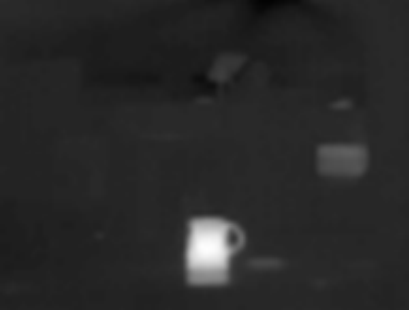
\includegraphics[width=.30\textwidth]{linearAGCa}} \quad
    \subfloat[][\emph{Classic Histogram Equalization}.\label{subfig:histrogram}]
        {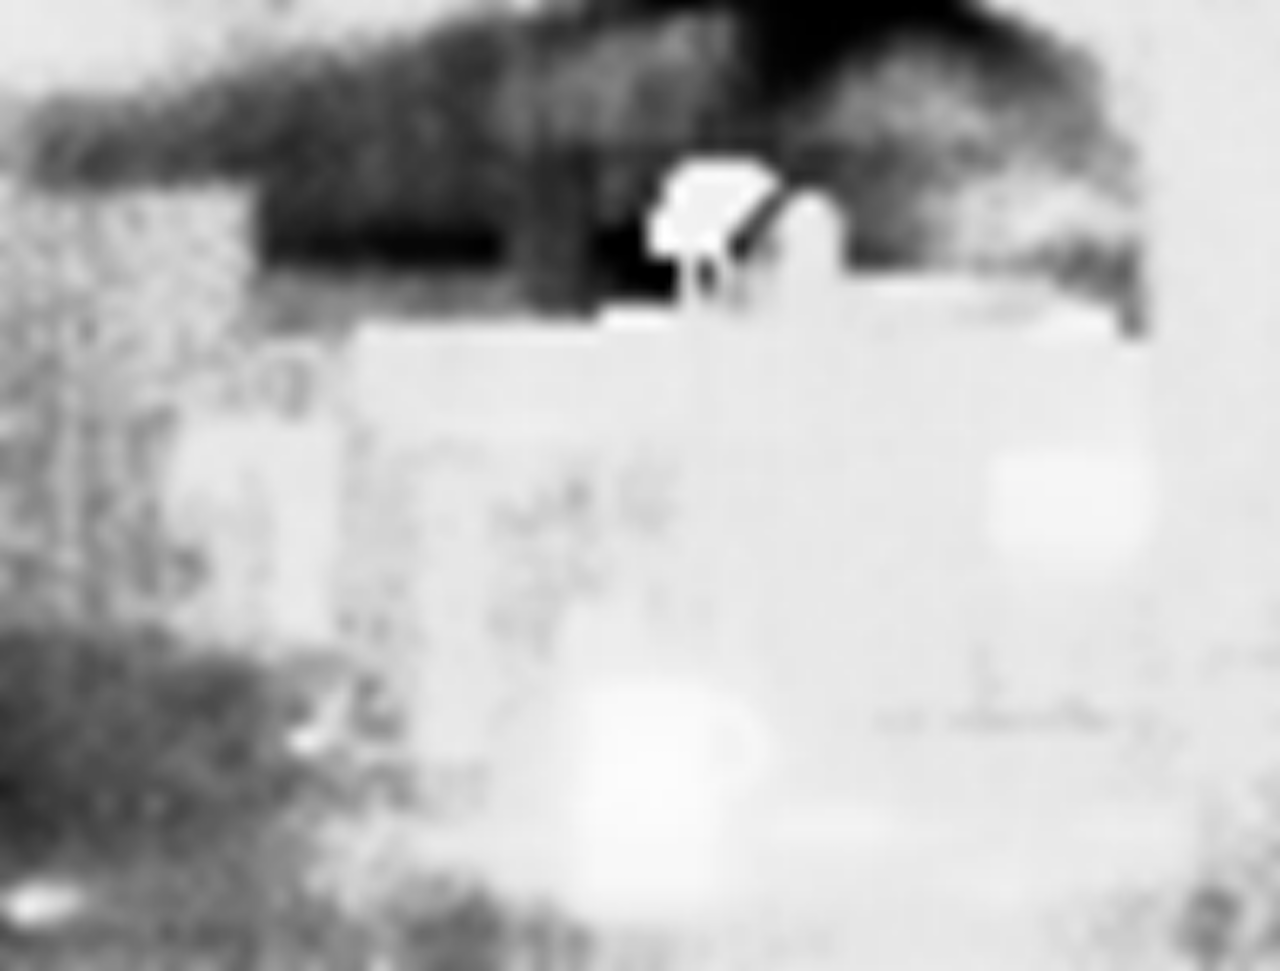
\includegraphics[width=.30\textwidth]{linearAGCb.png}} \quad
    \subfloat[][\emph{Lepton's Variant of HistogramEqualization}.\label{subfig:varianhistograms}]
        {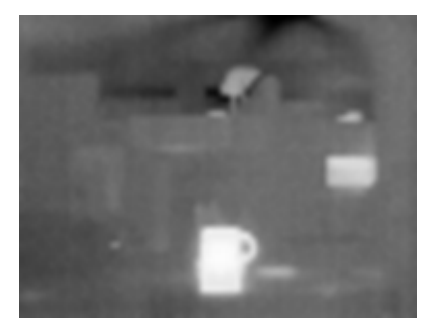
\includegraphics[width=.30\textwidth]{linearAGCc.png}}
    \caption{Comparison of Linear AGC and Classic/Lepton Variant of Histogram Equalization}
    \label{fig:comparisionlinearAGC}
\end{figure}
%
A high value of clip limit high results in a mapping more like classic histogram
equalization, whereas a low value results in mapping more like linear AGC. For
clip limit low, the opposite is true: a high value results in a mapping more
like linear AGC, whereas a low value results in a mapping more like classic
histogram equalization. The default values of both parameters produce a good
compromise between the two; however, because optimum AGC is highly subjective
and often application dependent, customers are encouraged to experiment to find
settings most appropriate for the target application. By default, the histogram
used to generate Lepton's 14-bit to 8-bit mapping function is collected from the
full array. In some applications, it is desirable to have the AGC algorithm
ignore a portion of the scene when collecting the histogram. For example, in
some applications it may be beneficial to optimize the display to a region of
interest (ROI) in the central portion of the image. When the AGC ROI is set to a
subset of the full image, any scene content located outside of the ROI is not
included in the histogram and therefore does not affect the mapping function
(note: this does not mean the portion outside of the ROI is not displayed or
that AGC is not applied there, only that those portions outside the AGC ROI do
not influence the mapping function).
%
%
\section{Interface}
\label{sec:lepton-interface}
The Raspberry Pi seen in section (\ref{sec:raspi3}) has bi-directional I/O pins, which you can use to drive LEDs, spin motors, or read button presses.
The board offers its GPIO over a standard male header on the board. Over the years the header has expanded from 26 pins to 40 pins while maintaining the original pinout.
There are at least two, different numbering schemes you may encounter when referencing pin numbers:
\begin{enumerate}
\item Broadcom chip-specific pin numbers 
\item \texttt{P1} physical pin numbers.
\end{enumerate} 
Here's a figure \ref{fig:gpio} showing all 26 pins on the \texttt{P1} header, including any special function they may have, and their dual numbers.
%
%
\begin{figure}[htb]
	\centering
	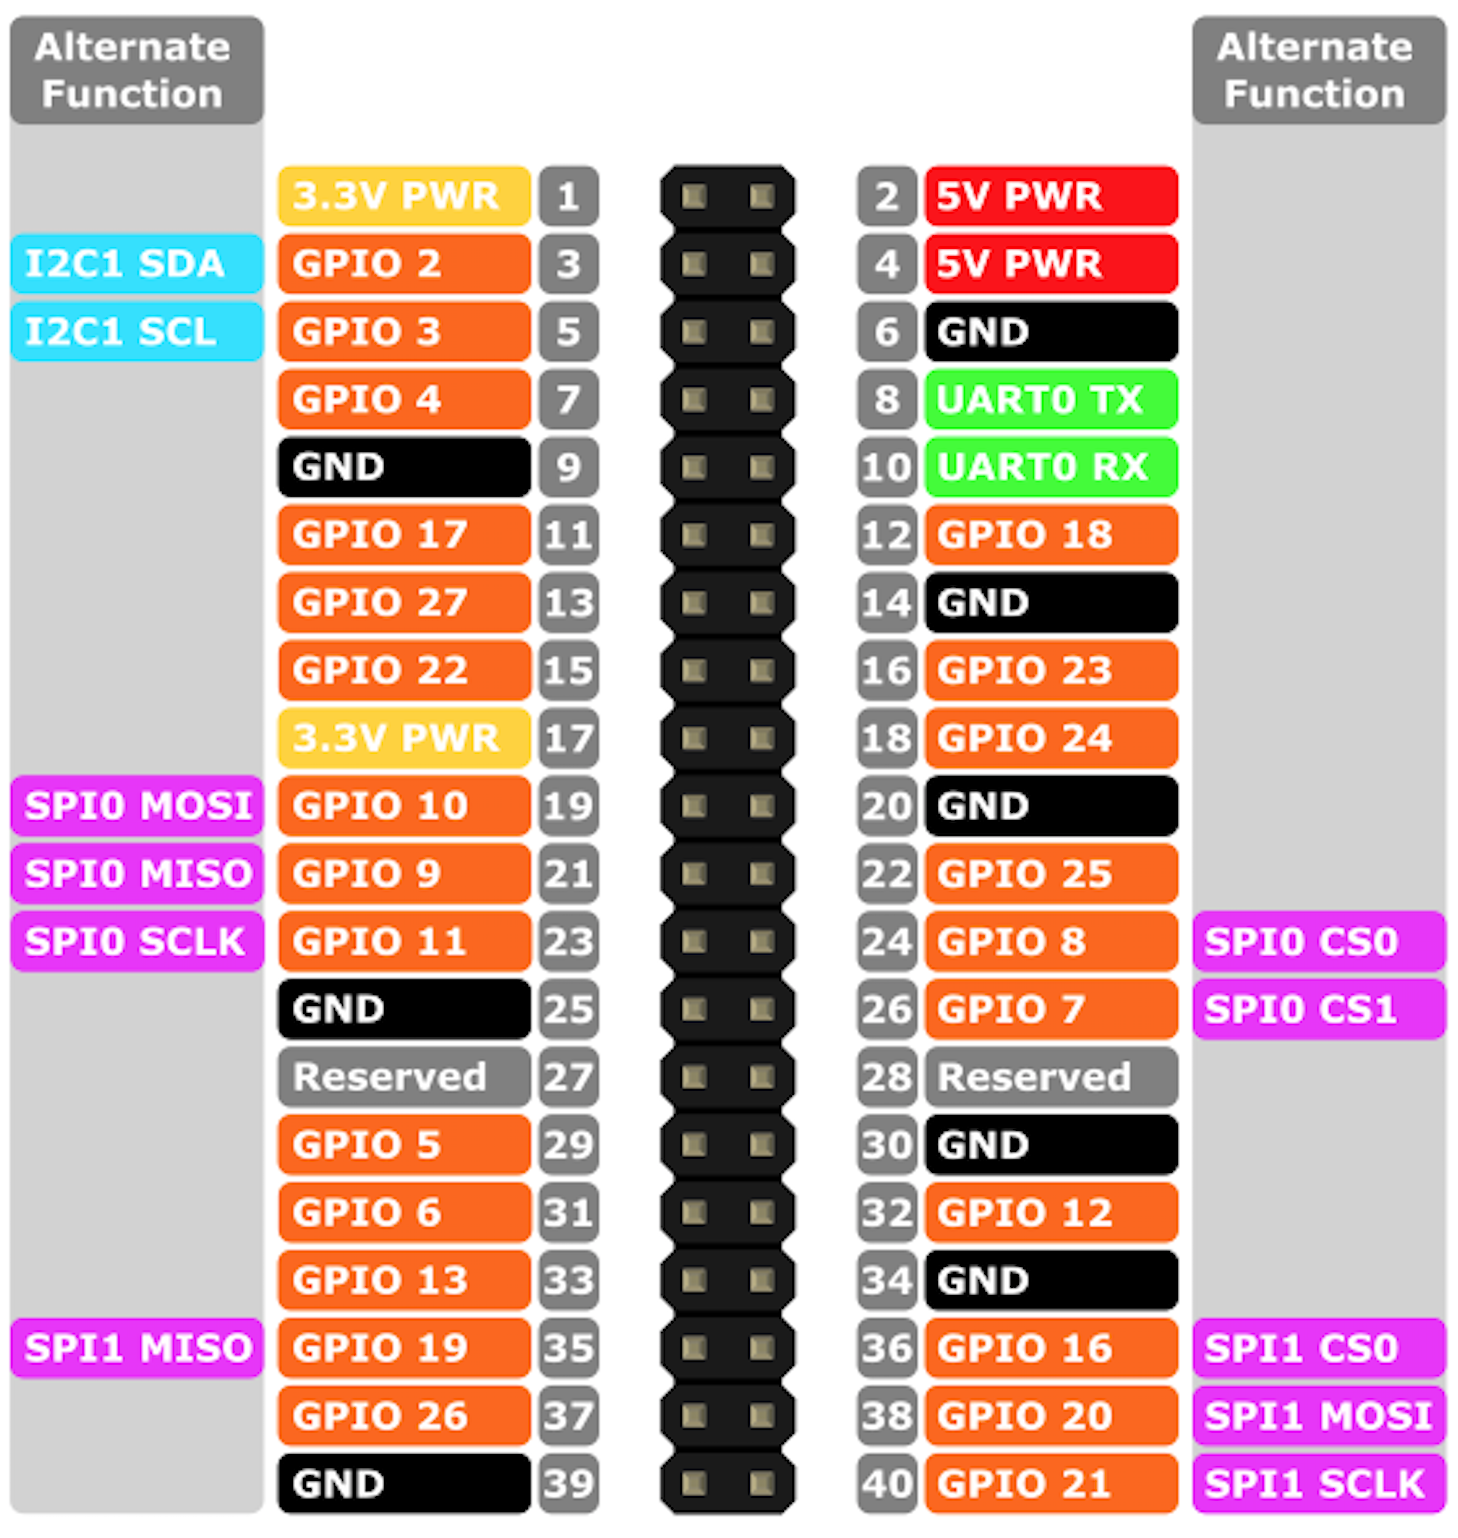
\includegraphics[width=0.45\textwidth]{gpio.png}
	\captionsource{Raspberry Pi 3 Pin Mappings.}{\href{https://docs.microsoft.com/es-es/windows/iot-core/learn-about-hardware/pinmappings/pinmappingsrpi}{Microsoft Windows Dev Center}}
	\label{fig:gpio}
\end{figure}
%
\newline The camera uses two interfaces for communication:
\begin{itemize}
\item \textbf{SPI} for transferring video frames from the camera to a SPI\footnote{SPI – Serial peripheral interface bus} master device.
\item \textbf{I$^2$C} for receiving control commands from the I$^2$C\footnote{I2C (Inter-integrated circuit)} master device.
\end{itemize}
The Raspberry Pi's CPU  has enough processing power to maintain smooth operation without delays, which turned out to be crucial for maintaining synchronization with the camera module when transferring video frames.
Below is reported the connection scheme used between the
FLIR breakout and the Raspberry Pi 's GPIO according to the figures (\ref{fig:brekout-gpio}) and the table (\ref{tab:scheme-gpio}).  

\begin{table}[!h]
	\centering
	\begin{tabular}{l c c l}
		\hline
		Raspberry GPIO	& Breakout board & 	Alternative function &	PIN \\
		\hline
		+3.3V			& 	VIN			 &	 SPI0 				 &	1	\\
		\rowcolor{aliceblue!85}SDA				& 	SDA			 &	 SPI0 				 &	3	\\
		SCL				& 	SCL			 &	 SPI0 				 &	5	\\
		\rowcolor{aliceblue!85}GND				& 	GND			 &	 SPI0 				 &	6 	\\
		MOSI			& 	MOSI		 &	 GND  				 &	19	\\	
 		\rowcolor{aliceblue!85}MISO			& 	MISO		 &	 3.3V 				 &	21	\\	
 		SCLK			& 	CLK			 &	 I2C1 				 &	23	\\
 		\rowcolor{aliceblue!85}CE0				& 	CS			 &	 I2C1 				 &	24	\\
 		\hline
	\end{tabular}
	\caption{Schematic connection GPIO}
	\label{tab:scheme-gpio}
\end{table}
%
\begin{figure}[htb]
    \centering
    \subfloat[][\emph{Breakout board detail}.\label{subfig:detail-breakout}]
        {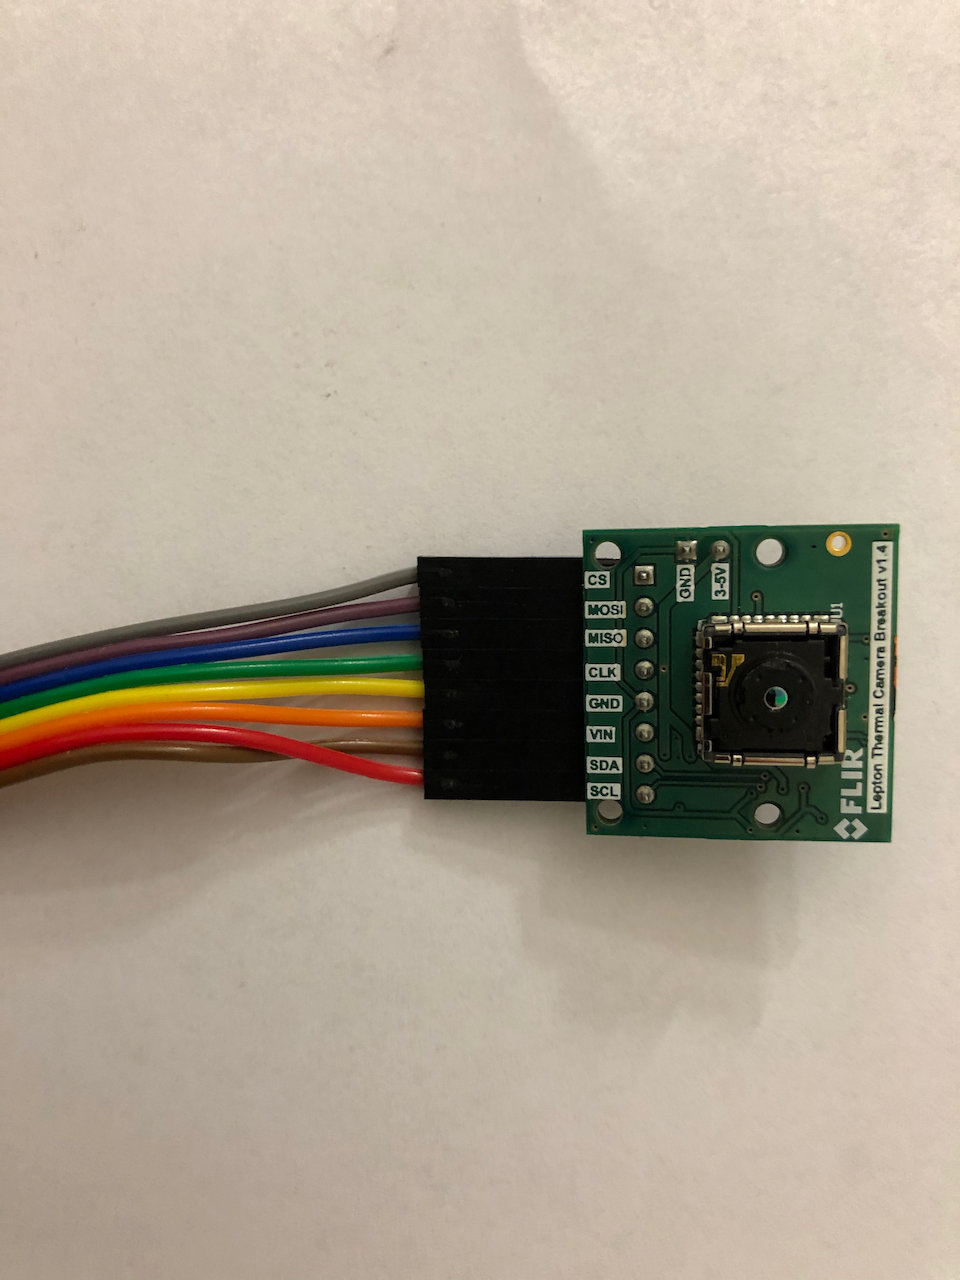
\includegraphics[width=.40\textwidth]{IMG_0361.jpg}} \quad
    \subfloat[][\emph{Top view}.\label{subfig:top.view-gpio}]
        {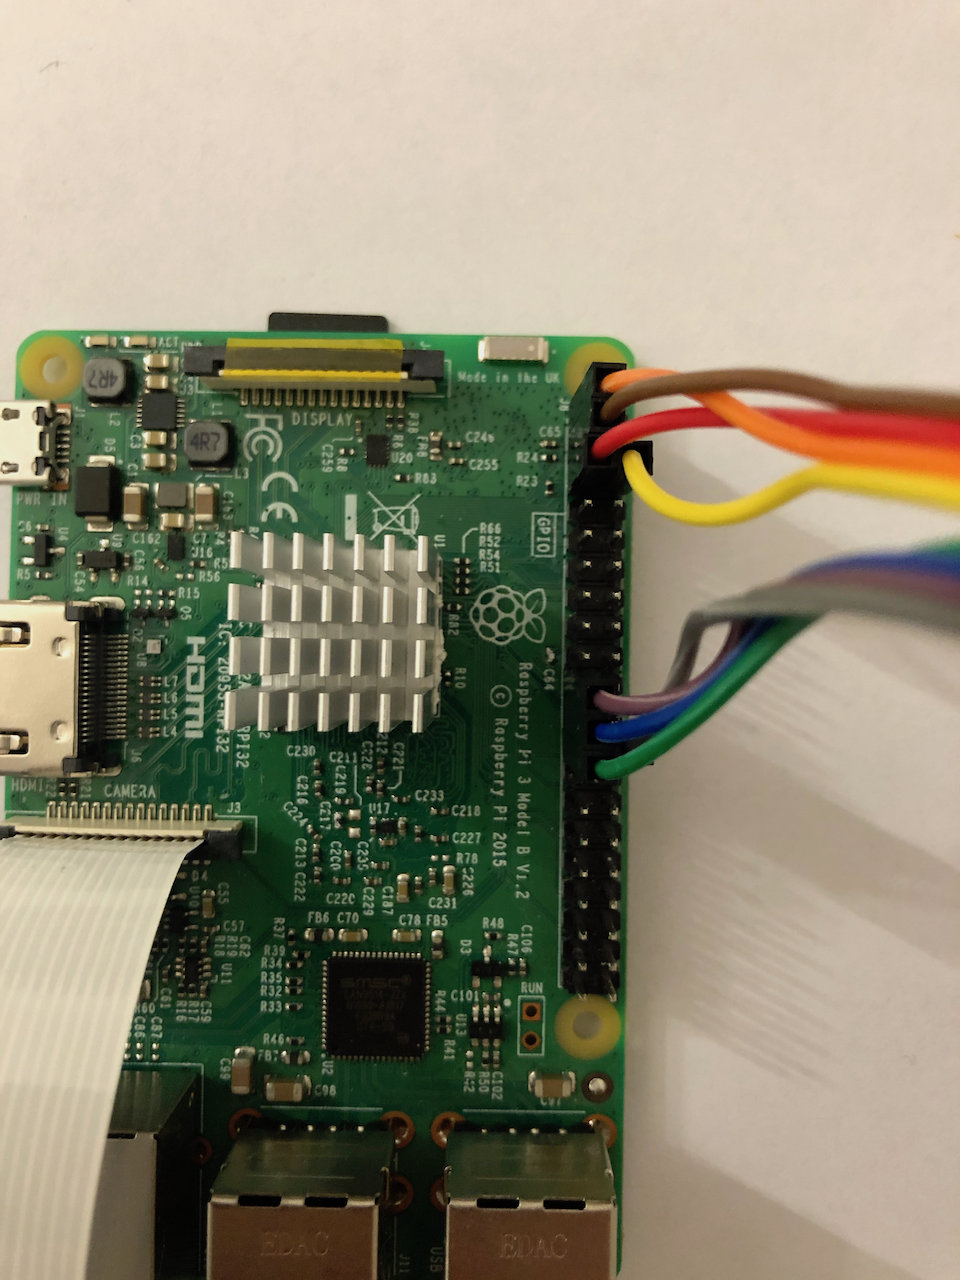
\includegraphics[width=.40\textwidth]{IMG_0362.jpg}} \\
            \subfloat[][\emph{Frontal view}.\label{subfig:front-view-gpio}]
        {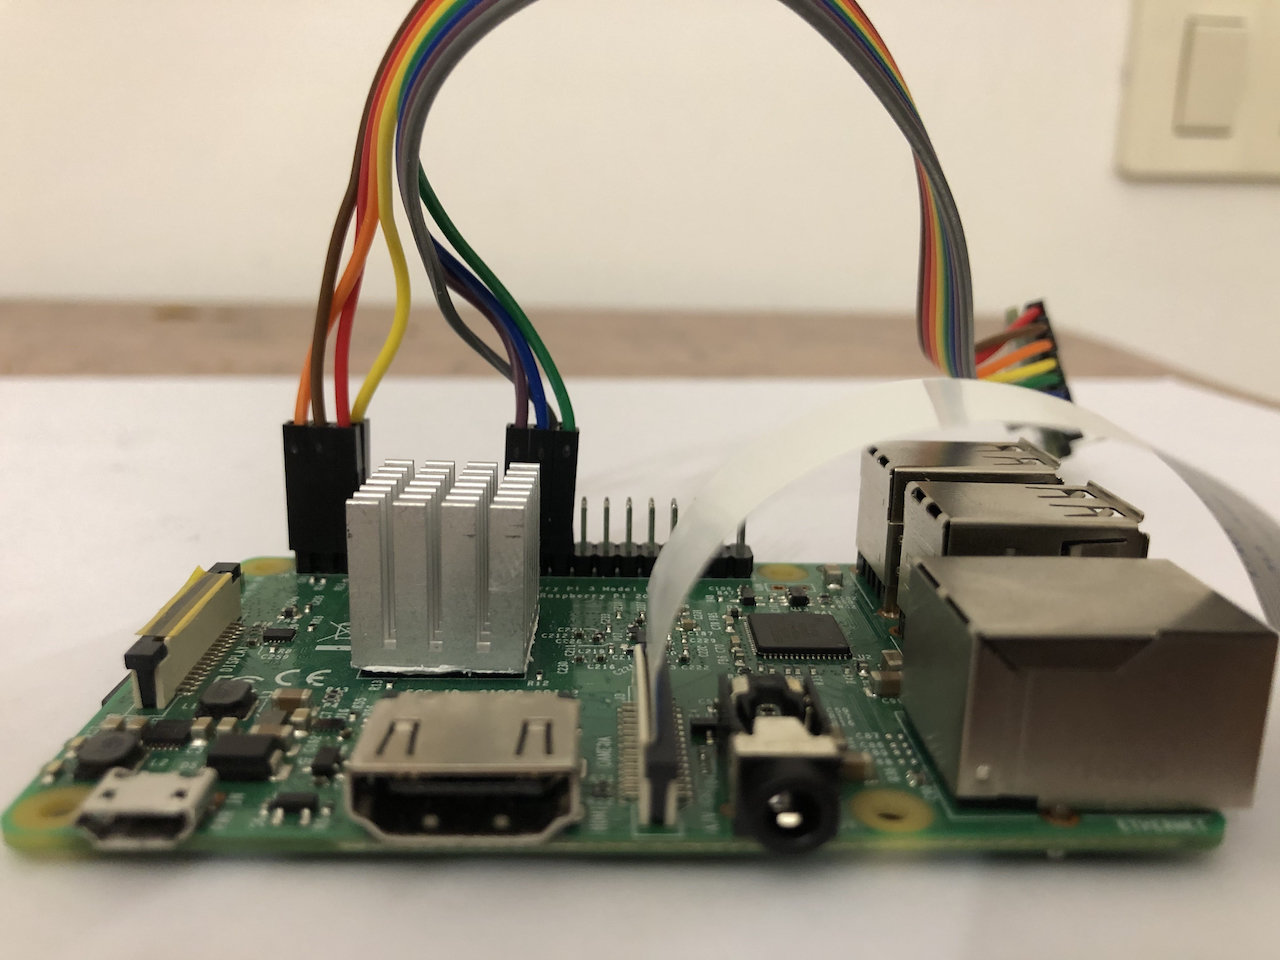
\includegraphics[width=.5\textwidth]{IMG_0360.jpg}}
    \caption{Realization of the connection between the Raspberry Pi 3 GPIO and Break out board}
    \label{fig:brekout-gpio}
\end{figure}

\section{Coral Dev-Board}
\label{sec:hard-devboard}
The Coral Dev Board is a single-board computer that contains an Edge TPU
coprocessor. It's ideal for prototyping new projects that demand fast on-device
inferencing for machine learning models.
%
\begin{figure}[htb]
	\centering
  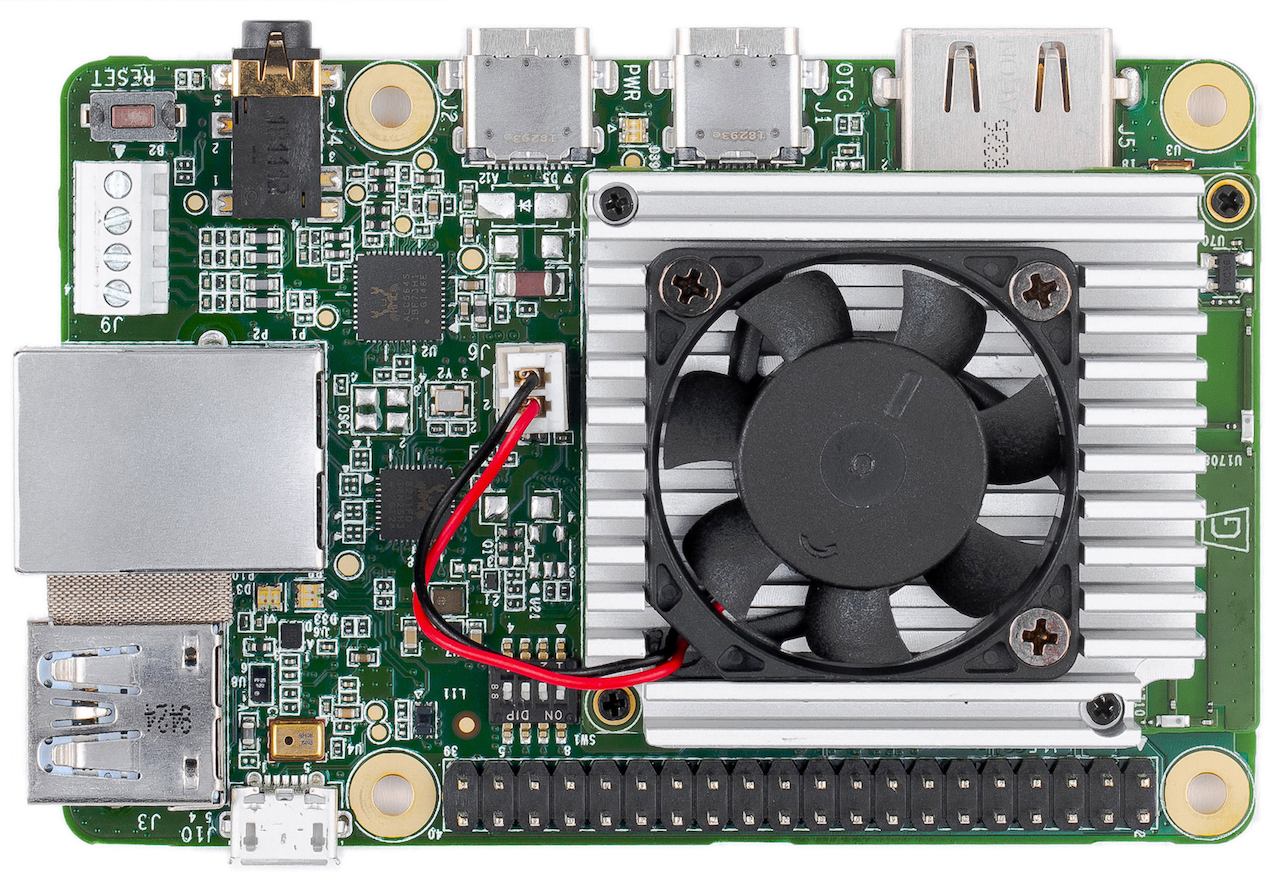
\includegraphics[width=0.80\textwidth]{devboard-dimensions.jpg}
  \captionsource{Coral Dev Board.}{
  \href{https://coral.ai/docs/dev-board/get-started/}{https://coral.ai/docs/dev-board/get-started/}}
  \label{fig:dev-board}
\end{figure}
%
\subsection{Overview}
\label{ssec:hard-devboard-overview}
The Coral Dev Board is a single-board computer that's ideal when you need to
perform fast machine learning (ML) inferencing in a small form factor. You can
use the Dev Board to prototype your embedded system and then scale to production
using the on-board Coral System-on-Module (SoM) combined with your custom PCB
hardware. The SoM provides a fully-integrated system, including NXP's iMX 8M
system-on-chip (SoC), eMMC memory, LPDDR4 RAM, Wi-Fi, and Bluetooth, but its
unique power comes from Google's Edge TPU coprocessor. The Edge TPU is a small
ASIC designed by Google that provides high performance ML inferencing with a low
power cost. For example, it can execute state-of-the-art mobile vision models
such as MobileNet v2 at almost 400 FPS, in a power efficient manner. 
The baseboard provides all the peripheral connections you need to prototype a
project, including USB 2.0/3.0 ports, DSI display interface, CSI-2 camera
interface, Ethernet port, speaker terminals, and a 40-pin I/O header. \hfill \break
Key benefits of the Dev Board:
\begin{itemize}
	\item High-speed and low-power ML inferencing (4 TOPS @ 2 \si{\watt})
	\item A complete Linux system (running Mendel, a Debian derivative)
	\item Prototyping and evaluation board for the small Coral SoM (40 x 48 \si{\milli\meter})
\end{itemize}
%
\begin{table}[htb]
	\centering
	\begin{tabular}{c}
	\hline \\
Edge TPU System-on-Module (SoM)\\
% NXP i.MX 8M SoC (Quad-core Arm Cortex-A53, plus Cortex-M4F)
% Google Edge TPU ML accelerator coprocessor
% Cryptographic coprocessor
% Wi-Fi 2x2 MIMO (802.11b/g/n/ac 2.4/5 GHz)
% Bluetooth 4.2
% 8 GB eMMC
% 1 GB LPDDR4
% USB connections
% USB Type-C power port (5 V DC)
% USB 3.0 Type-C OTG port
% USB 3.0 Type-A host port
% USB 2.0 Micro-B serial console port
% Audio connections
% 3.5 mm audio jack (CTIA compliant)
% Digital PDM microphone (x2)
% 2.54 mm 4-pin terminal for stereo speakers
% Video connections
% HDMI 2.0a (full size)
% 39-pin FFC connector for MIPI DSI display (4-lane)
% 24-pin FFC connector for MIPI CSI-2 camera (4-lane)
% MicroSD card slot
% Gigabit Ethernet port
% 40-pin GPIO expansion header
% Supports Mendel Linux (derivative of Debian)
\hline
	\end{tabular}
	\caption{Coral Dev Board Features.}
	\label{tab:hard-devboard-spec}
\end{table}
%
\noindent The Google Coral with a special TPU chip
performing all tensor calculationsworks with special 
pre-compiled TensorFlow Lite networks. If the topology of the neural network and
its required operations can be described in TensorFlow it may work well on the
Google Coral. However, with its sparse 1 Gbyte RAM, memory shortage can still be
an issue. The Google USB accelerator has its special back-end compiler
converting a TensorFlow Lite file to an executable model for the dongle
TPU.
% 
%
\section{TPU explained in depth}
\label{sec:hard-tpu}
% cite page https://qengineering.eu/google-corals-tpu-explained.html
The Google Coral has a TPU on board which speeds up the tensor calculations
enormously. These tensor calculations are used in deep learning and neural
networks. \hfill \break 
The Google Coral Dev board use an ASIC made by the Google team called the Edge 
TPU. It is a much lighter version of the well-known TPUs used in Google's 
datacenter. \hfill \break
It also consumes very little power, so it is ideal for small embedded systems. 
Nevertheless, the similarities in applied technology are significant.\cite{TPU:explained} 
%
\subsection{Neural Node}
\label{ssec:hard-neural-node}
Neural networks used in deep learning consists of many neural nodes. They are
all connected together in a defined way. The way these nodes are wired is
called the topology of the network. This topology determines the function the
network performs. See this list for a selection of several types of deep
learning networks. Each node has always three basic components. 
A multiplier multiplies all the inputs with their respective so-called weight,
the synapses. An adder who accumulates all the individual multiplications. And
an activation function that shapes the output given the addition. A schematic
view below (\ref{fig:neuron}).\hfill \break
%
\begin{figure}[htb]
	\centering
  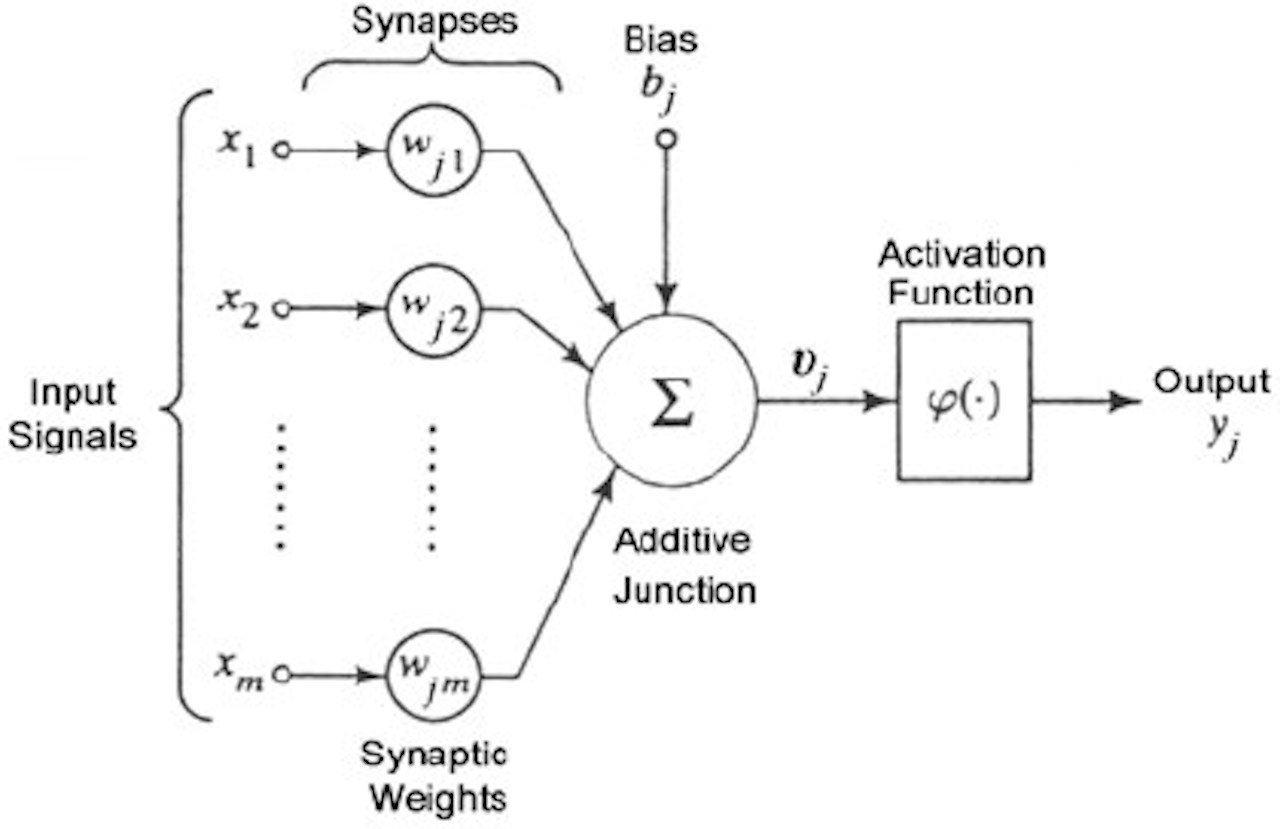
\includegraphics[width=0.70\textwidth]{sinapse.jpg}
  \captionsource{Artificial Neuron models and its parts.}{Adapted from Haykin (1994)}
  \label{fig:neuron}
\end{figure}
%
\newpage
\noindent The formula can be written as follows \eqref{eq:neuron}.
\begin{equation}
\label{eq:neuron}
	y_{i} = \phi \, \left(\sum_{i=1}^{n} w_{ij}\cdot x_{i} \right)
\end{equation}
%
Deep neural network is consist of millions of neural nodes distribute over many
layers; despite the simplicity of the operation, only on multiplication and one
addition, require long compute time to obtain a result. keep in mind that for
training a network requires many epochs. In other words, the main problem is
time. The algorithms is well suited for parallel execution. Although
distributing the algorithm over the processes and threads can be an option
actually provides disappoint results for the presence of bottlenecks due to
architecture general purpose. On the other hand use of Graphical Processing
Unit, the GPU on video card designed for efficient manipulation memory. Their
highly parallel structure make them more efficient respect CPU especially for
algorithms that process large blocks of data in parallel. The best choice is the
use of the Tensor Processing Unit, the TPU. This device has been specially
designed for the above neural node algorithm.
%
\subsection{The adder}
\label{ssec:hard-adder}
Generally a strategy adopted when software is tool slow is modify the hardware
to reach the better achievements.
The structure inside TPU is realized by three main components derived from 
neural node, then keeping in mind the scheme in figure (\ref{fig:neuron}): the 
\textbf{multiplier}, the \textbf{adder} and the \textbf{activation function} 
must be included in the hardware.
Start with analysing the diagram of the 4-bit adder realized in figure
(\ref{fig:4-bit-adder}).
Where: \texttt{A} and \texttt{B} are the inputs. If the output overflows 
\texttt{C4} the carry out is set. \texttt{C0} is the carry-in of a previous 
phase.\cite{TPU:explained}
%
\begin{figure}[!h]
	\centering
  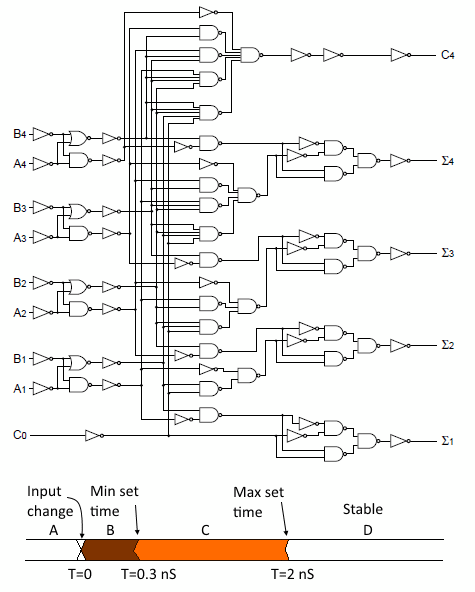
\includegraphics[width=0.75\textwidth]{Adder1.png}
  \captionsource{4-bit adder}{\href{https://qengineering.eu/google-corals-tpu-explained.html}{Q-engineering}}
  \label{fig:4-bit-adder}
\end{figure}
%
Signals \texttt{A} and \texttt{B} propagate through the circuit and generate the
result \texttt{A + B}. Changing one of them alters almost immediately the
output. This happens extremely very fast, within a few nanoseconds. This
propagation time depends on the number of digital ports whose output changes.
The propagation time is therefore not fixed, but lies between two limits, a
minimum and a maximum time, see diagram at the bottom of the drawing
(\ref{fig:4-bit-adder}). By the way, al mentioned times are illustrative and
have no relationship to any device.\cite{TPU:explained}
%
\newpage
\subsection{Pipeline}
\label{ssec:hard-pipeline}
Consider the example where: the propagation time of one adder is $2 \,
\si{\nano\second}$, therefore the maximum clock rate can be $500
\,\si{\mega\hertz}$. Taking into account that a neural node can have many
inputs, also hundreds, that must be accumulated this affect the propagation time
that increase dramatically. This implies that the last adder in the chain must
be attend all intermediate result before its output becomes stable.
If we consider a chain of 250 input each of one with $2\, \si{\nano\second}$
delay, we obtain total time of $500 \,\si{\nano\second}$ waiting. \\
Consequently clock results extremely slow $2\,\si{\mega\hertz}$, then solution
adopted is structured pipeline where between each adder is inserted a memory
element that keep keeps the result stable for the next adder. 
As show in figure (\ref{fig:4-bit-adder-register}). \hfill \break
%
\begin{figure}[!h]
	\centering
	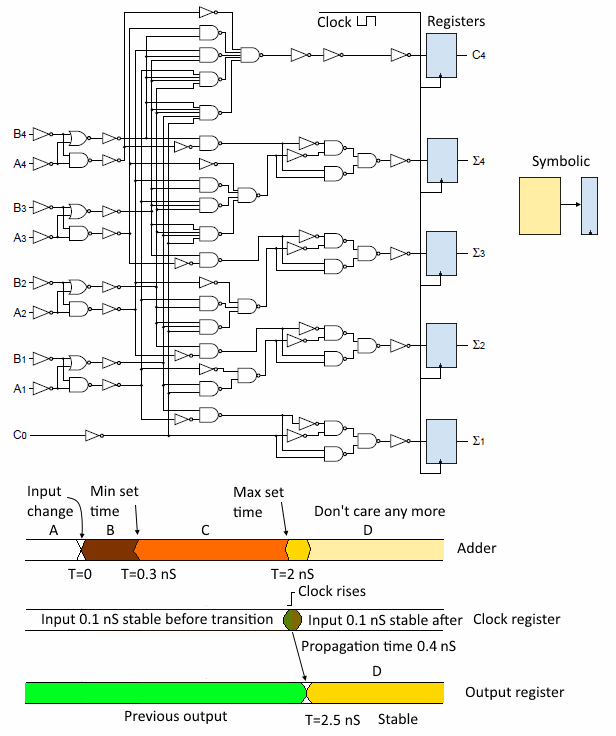
\includegraphics[width=0.75\textwidth]{AdderReg10.png}
	\captionsource{4 bit adder with register}{\href{https://qengineering.eu/google-corals-tpu-explained.html}{Q-engineering}}
	\label{fig:4-bit-adder-register}
\end{figure}
%
\break The output of the registers is updated at the rising edge of the clock
signal. 
That is the only time the output can change. When the clock signal is high or
low, the inputs cannot manipulate the output, then it remains stable. 
Just before the clock rises, the input must be stable for a minimum time, also
just after the rise time. 
In contrast to the previous example, now consider a delay of $0.1
\,\si{\nano\second}$ and adding the register's propagation time of $(0.4
\,\si{\nano\second})$, the total propagation reach for a new stable signal is
now $2.5 \si{\nano\second}$, which results increasing up to clock speed of $400
\,\si{\mega\hertz}$. Observable in figure (\ref{fig:pipe}).
%
\begin{figure}[htb]
	\centering
	\includegraphics[width=0.60\textwidth]{pipe10.png}
	\captionsource{Digital pipeline.}{\href{https://qengineering.eu/google-corals-tpu-explained.html}{Q-engineering}}
	\label{fig:pipe}
\end{figure}
%
%
Taking into account the table in figure \ref{fig:pipe}, each color represents a
value. After four clock cycles, the value at the input has propagated through
the network and appears at the output.
Because the registers are updated simultaneously a new input is accepted every
$2.5 \,\si{\nano\second}$. The propagation time has been restored. 
The time it takes to travel through the whole pipeline is called latency time
and is $10 \,\si{\nano\second}$ in the above diagram $(4 \times 2.5
\,\si{\nano\second}$). 
Every digital component is built on large pipelines which guarantee the required
speed.\cite{TPU:explained}
%
\subsection{The mul-add cell}
\label{ssec:The-mul-add-cell} 
The input signal of every neural node has effect on final result.
This gives a simple multiplication for an input mediate by a weight value. 
The operation of multiplication can be implemented with same logic of an adder,
then are necessary more gates.
Remembering that the neural node has multiplied his value for weight value. 
Thus the representation assume the scheme in figure
(\ref{fig:mul-add-register}). \hfill \break
%
\begin{figure}[htb]
	\centering
	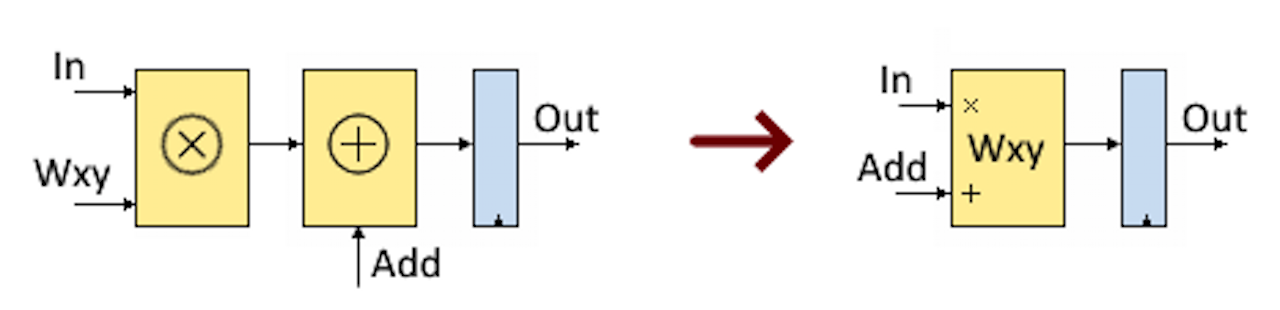
\includegraphics[width=0.65\textwidth]{MulAddReg10.png}
	\captionsource{Mul-Add register.}{\href{https://qengineering.eu/google-corals-tpu-explained.html}{Q-engineering}}
	\label{fig:mul-add-register}
\end{figure}
%
%
%\break For the sake of simplicity, no additional propagation time fixing registers have
%been added. With the formula of the neural node in mind, it is now relatively
%easy to design such a neuron with a few mul-add cells. Below the schematic for a
%three input neuron.
%
\begin{figure}[htb]
	\centering
	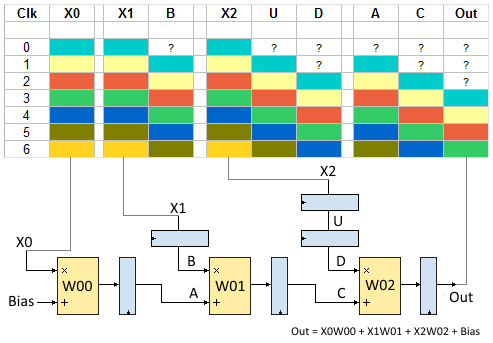
\includegraphics[width=0.75\textwidth]{Neuron.png}
	\captionsource{schematic for a
three input neuron.}{\href{https://qengineering.eu/google-corals-tpu-explained.html}{Q-engineering}}
	\label{fig:3-input-neuron}
\end{figure}
%
%
\newline
Are necessary many important clarifications about the input registers
\texttt{X1} and \texttt{X2} displayed in figure (\ref{fig:3-input-neuron}). They
generate a delay line in the \emph{mul-add} chain, thus can permit to correct
synchronize. Considering the second cell \emph{mul-add} who sum the output from
previous cell (signal \texttt{A}) retarded by one clock cycle. Consequently also
the multiplication between the value in register \texttt{X1} and weight value
must be delayed the same amount of time. The schema reported in figure
(\ref{fig:3-input-neuron}) shows for each colour that represent the vector of
input \texttt{$[X0, X1, X2]$} while the input \texttt{A} and \texttt{B},
represented by lines straight, maintains always same colour. This means that
they appear simultaneous, i.e. are synchronised. The same must be valid for
input \texttt{C} and \texttt{D}.
%
\subsection{Systolic array}
\label{ssec:hard-systolic-array}
Starting from structure, just examined, is quite easy extend it to other neurons, taking into account that every single input is connected with all neurons in the next layer, as shows in figure (\ref{fig:systolic-array-edge-tpu}).
%
\begin{figure}[htb]
	\centering
	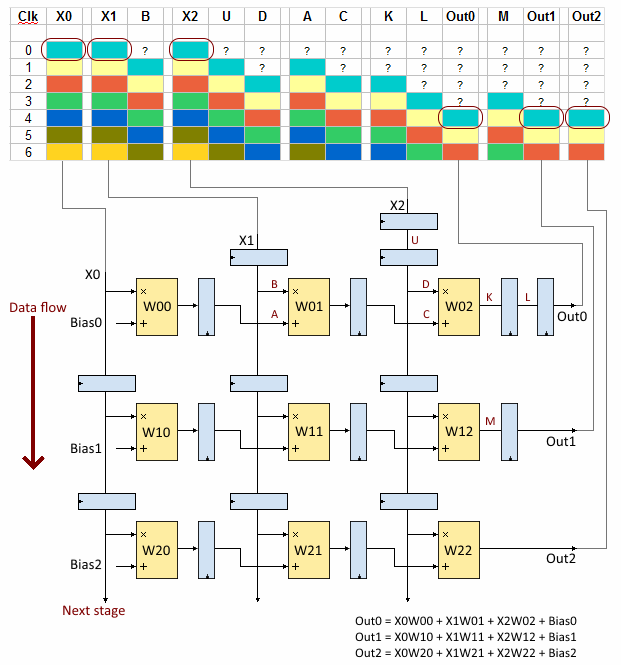
\includegraphics[width=0.65\textwidth]{Systolic-Array.png}
	\captionsource{Systolic Array Edge TPU.}{\href{https://qengineering.eu/google-corals-tpu-explained.html}{Q-engineering}}
	\label{fig:systolic-array-edge-tpu}
\end{figure}
%
%
The adoption of this solution, called systolic array, permits to have an
increment of speed in parallel calculation. 
Since the propagation time remains unchanged for an spread of systolic array in
depth or width, while only the latency time grows up this represent the solution
widely used for neural network hardware.
%
%The sizes of the systolic array in the Edge TPU are not known yet. The first TPU
%Google uses in its datacenter contains 256 x 256 \emph{mul-add} cells. Running at 700
%MHz it can theoretical performs 256 x 256 x 700.000.000 = 46 trillion \emph{mul-adds}
%per second. Or if you look to individual operations 92 trillion (92 TOPS).
%However, this impressive figure is purely theoretical. In practice, there are
%some factors that slow performance.
%
%The systolic array is made up of hardware. This means that it has fixed
%dimensions. Therefore, the input and output vectors also have fixed dimensions.
%However, the numbers of neurons per layer are determined by the design and are
%certainly not constant. If the number is smaller than the size of the array, it
%is, of course, possible to expand an input vector with leading zeros, so that
%the dimension equals the array size. The same technique can be applied to an
%oversized output vector.
%
%If the input vector contains more elements than the width of the systolic array,
%the entire arithmetic calculation must be performed in more than one call. To
%this end, the input vector is cut into a series of smaller vectors that match
%the width of the series. They are then processed one after the other. The
%intermediate results must be stored in a buffer. These values must be added
%after completion of all the systolic calls. Note that not only the input vector
%is split into smaller parts, but all weights used in the multiplication must be
%updated according to the formula's processing section. This may require a
%massive memory transfer. Below an example of a systolic array with only four
%inputs processing a vector of size 12.
%
%
%
%Looking at Google's schematic overview of the TPU, these output buffers and
%accumulators are drawn at the bottom. (In their diagram, the output is at the
%bottom instead of the right as on our drawing).
%Google TPU detail
%
% 
%Buffers have also been placed on the input vector side in the diagram above.
%They act as a first-in-first-out buffer, a FIFO. This guarantees continuous
%input of the systolic array with input values. It may also have some rotating
%operations, which increases the performance of CNN networks. It is unclear
%whether Google uses this method here. 
%
\subsection{Activation unit}
\label{ssec:activation-unit}
Once the output is available, it is sent to the activation unit. This module
within the Edge TPU applies the activation function to the output. It is
hardwired. In other words, you cannot alter the function, it works like a ROM.
Probably it is a ReLU function as it is nowadays the most used activation
function and it is very easy to implement in hardware.\cite{TPU:explained}
%
% 
% TPU versus Edge TPU. The Google's Edge TPU is a much smaller device than the
% TPUs that Google uses in its data centers. Below the PCB with the original TPU
% and the Edge TPU on the same scale. TPU vs Edge TPU It is obvious that such a
% small device cannot have the same functions as its much larger ancestor. The
% floor plan on the die does not allow this to happen. Nor can the systolic
% array have the $256 \times 256$ dimension as in the original TPU. Google has
% so far not revealed the measures in the Edge, but a well-founded estimate is
% $64 \times 64$ with a clock of $480 \si{\mega\hertz}$, resulting in 4 TOPS.
% Memory is also an issue. In the original chip, it takes around $29\%$ of the
% total floor plan. It is impossible that the same amount can be found on the
% Edge TPU die. Moreover, the chip is very energy efficient. It requires no
% cooling. This means that almost certainly all the buffering is outside the
% chip. It leaves only a simple transfer of input vectors, output vectors and
% weights to the chip.  Practice. In fact, that is the whole concept of the
% Google Coral Dev board. Transfer all tensor calculations to the TPU as quickly
% as possible, fetch for the results, fill them in the next layer and start the
% cycle again with this layer. Process all layers one by one until they are
% ready. To speed up the process, TensorFlow uses a special back end compiler,
% the Edge TPU compiler. The main task of this Edge TPU compiler is to partition
% the TensorFlow Lite file into more suitable TPU transfer packages. If for any
% reason the TPU cannot process the TensorFlow Lite file or part of it, the CPU
% will take care of it. However, if this happens, your application will, of
% course, work extremely slowly. 8 bits integers. Another way of speeding up the
% calculations is the use of 8 bit signed integers instead of floats. A floating
% number occupies 32 bits in memory whereas the integer only needs 8. Because a
% neural network is fairly insensitive to number accuracy, it will also work
% well with 8-bit integers. It will still remain accurate. Not only does this
% technology save approximately $75\%$ memory, but it also significantly reduces
% the number of transistors on the chip. If you look at the adder at the top of
% the page, you can imagine how many transistors a floating-point adder needs.
% Without this compression, the Edge TPU would not be as powerful, small and
% energy efficient.

% The converting algorithm from floating point to 8 bit signed integer is quite
% simple. First, it determines which maximum and minimum a variable will take in
% the model. The larger of the two is then taken and scaled to 127. Suppose
% minimum is -1205.8 and maximum is 646.8. The larger is the min value of
% 1205.8. So that number becomes -127. Zero remains zero. That gives 646.8 a
% integer value of 127 x (646.8 / 1205.8) = 68. Every number in the TensorFlow
% model is converted in this way. Not only for the Edge TPU, by the way. All
% TensorFlow Lite models for embedded deep learning are processed in this way.

% A rather remarkable detail is the output of the Edge TPU, which does consist
% of a floating point. Because the activation function is embedded in a ROM, it
% is just as easy to store floating numbers as integers. One last tip in this
% regard. Apply quantization-aware training in TensorFlow. This simulates the
% effect of the 8 bit signed integers. Therefore generating a more precise
% model. It makes the model also more tolerant for low precision variables.
\section{TPU explained in depth}
\label{sec:hard-tpu}
% cite page https://qengineering.eu/google-corals-tpu-explained.html
The Google Coral has a TPU on board which speeds up the tensor calculations
enormously. These tensor calculations are used in deep learning and neural
networks. \hfill \break 
The Google Coral Dev board use an ASIC made by the Google team called the Edge 
TPU. It is a much lighter version of the well-known TPUs used in Google's 
datacenter. \hfill \break
It also consumes very little power, so it is ideal for small embedded systems. 
Nevertheless, the similarities in applied technology are significant.\cite{TPU:explained} 
%
\subsection{Neural Node}
\label{ssec:hard-neural-node}
Neural networks used in deep learning consists of many neural nodes. They are
all connected together in a defined way. The way these nodes are wired is
called the topology of the network. This topology determines the function the
network performs. See this list for a selection of several types of deep
learning networks. Each node has always three basic components. 
A multiplier multiplies all the inputs with their respective so-called weight,
the synapses. An adder who accumulates all the individual multiplications. 
And an activation function that shapes the output given the addition. A
schematic view below (\ref{fig:neuron}).\hfill \break
%
\begin{figure}[htb]
	\centering
	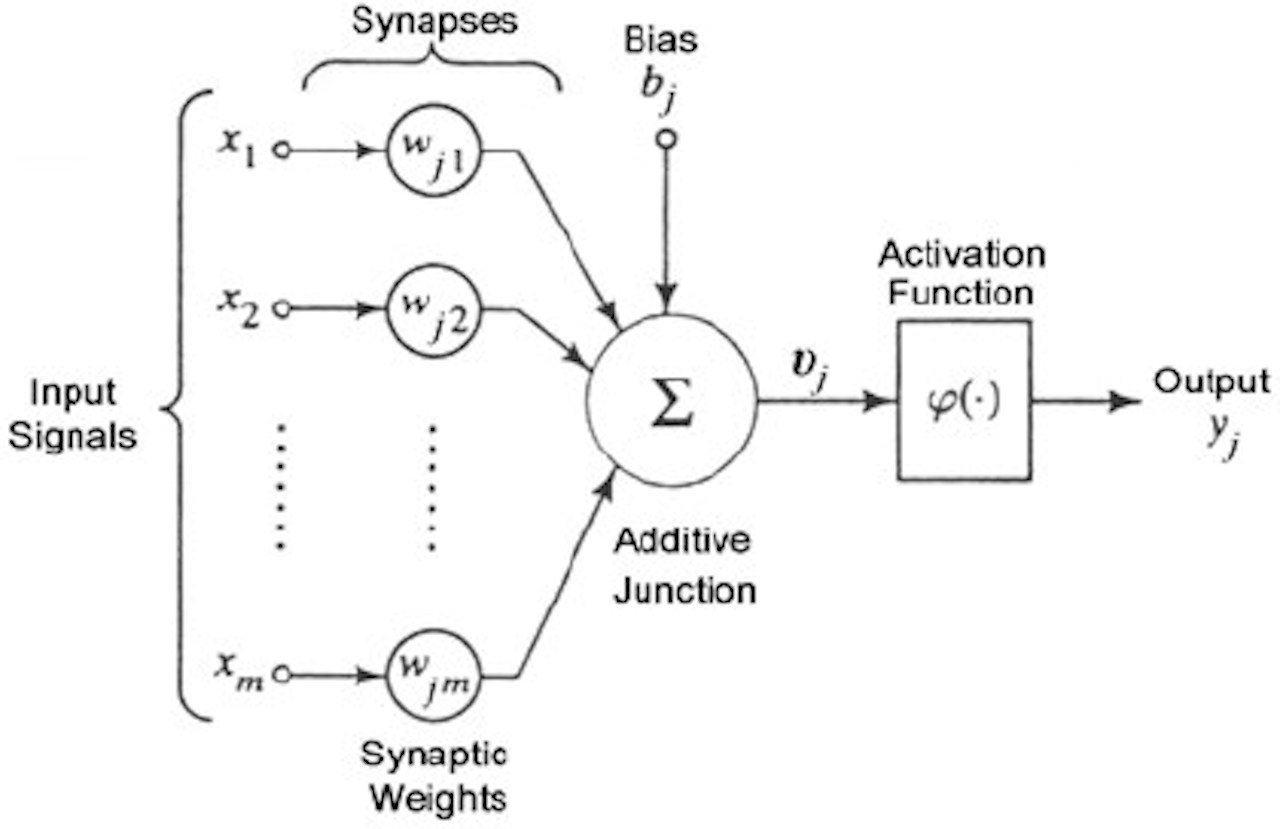
\includegraphics[width=0.70\textwidth]{sinapse.jpg}
	\captionsource{Artificial Neuron models and its parts.}{Adapted from Haykin (1994)}
	\label{fig:neuron}
\end{figure}
%
\newpage
\noindent The formula can be written as follows \eqref{eq:neuron}.
\begin{equation}
\label{eq:neuron}
	y_{i} = \phi \, \left(\sum_{i=1}^{n} w_{ij}\cdot x_{i} \right)
\end{equation}
%
Deep neural network is consist of millions of neural nodes distribute over many
layers; despite the simplicity of the operation, only on multiplication and one
addition, require long compute time to obtain a result. keep in mind that for
training a network requires many epochs. In other words, the main problem is
time. The algorithms is well suited for parallel execution. Although
distributing the algorithm over the processes and threads can be an option
actually provides disappoint results for the presence of bottlenecks due to
architecture general purpose. On the other hand use of Graphical Processing
Unit, the GPU on video card designed for efficient manipulation memory. Their
highly parallel structure make them more efficient respect CPU especially for
algorithms that process large blocks of data in parallel. The best choice is the
use of the Tensor Processing Unit, the TPU. This device has been specially
designed for the above neural node algorithm.
%
\subsection{The adder}
\label{ssec:hard-adder}
Generally a strategy adopted when software is tool slow is modify the hardware
to reach the better achievements.
The structure inside TPU is realized by three main components derived from 
neural node, then keeping in mind the scheme in figure (\ref{fig:neuron}): the 
\textbf{multiplier}, the \textbf{adder} and the \textbf{activation function} 
must be included in the hardware.
Start with analysing the diagram of the 4-bit adder realized in figure
(\ref{fig:4-bit-adder}).\hfill \break
Where: \texttt{A} and \texttt{B} are the inputs. If the output overflows 
\texttt{C4} the carry out is set. \texttt{C0} is the carry-in of a previous 
phase.\cite{TPU:explained}
%
\begin{figure}[!h]
	\centering
	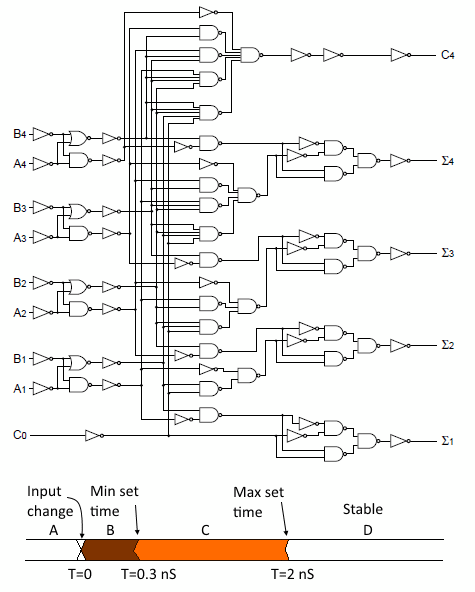
\includegraphics[width=0.75\textwidth]{Adder1.png}
	\captionsource{4-bit adder}{\href{https://qengineering.eu/google-corals-tpu-explained.html}{Q-engineering}}
	\label{fig:4-bit-adder}
\end{figure}
%
Signals \texttt{A} and \texttt{B} propagate through the circuit and generate the
result \texttt{A + B}. Changing one of them alters almost immediately the
output. This happens extremely very fast, within a few nanoseconds. This
propagation time depends on the number of digital ports whose output changes.
The propagation time is therefore not fixed, but lies between two limits, a
minimum and a maximum time, see diagram at the bottom of the drawing
(\ref{fig:4-bit-adder}). By the way, al mentioned times are illustrative and
have no relationship to any device.\cite{TPU:explained}
%
\newpage
\subsection{Pipeline}
\label{ssec:hard-pipeline}
Consider the example where: the propagation time of one adder is $2 \,
\si{\nano\second}$, therefore the maximum clock rate can be $500
\,\si{\mega\hertz}$. Taking into account that a neural node can have many
inputs, also hundreds, that must be accumulated this affect the propagation time
that increase dramatically. This implies that the last adder in the chain must
be attend all intermediate result before its output becomes stable. 
If we consider a chain of 250 input each of one with $2\, \si{\nano\second}$
delay, we obtain total time of $500 \,\si{\nano\second}$ waiting. \\ 
Consequently clock results extremely slow $2\,\si{\mega\hertz}$, then solution
adopted is structured pipeline where between each adder is inserted a memory
element that keep keeps the result stable for the next adder. 
As show in figure (\ref{fig:4-bit-adder-register}). \hfill \break
%
\begin{figure}[!h]
	\centering
	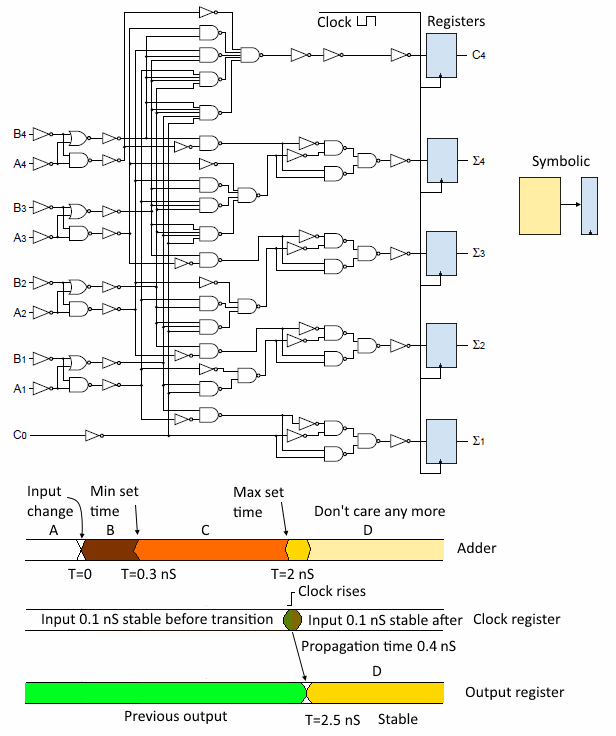
\includegraphics[width=0.75\textwidth]{AdderReg10.png}
	\captionsource{4 bit adder with register}{\href{https://qengineering.eu/google-corals-tpu-explained.html}{Q-engineering}}
	\label{fig:4-bit-adder-register}
\end{figure}
%
\break The output of the registers is updated at the rising edge of the clock
signal. That is the only time the output can change. When the clock signal is
high or low, the inputs cannot manipulate the output, then it remains stable. 
Just before the clock rises, the input must be stable for a minimum time, also
just after the rise time. In contrast to the previous example, now consider a
delay of $0.1 \,\si{\nano\second}$ and adding the register's propagation time of
$(0.4 \,\si{\nano\second})$, the total propagation reach for a new stable signal
is now $2.5 \,\si{\nano\second}$, which results increasing up to clock speed of
$400 \,\si{\mega\hertz}$. Observable in figure (\ref{fig:pipe}). \hfill \break
%
\begin{figure}[htb]
	\centering
	\includegraphics[width=0.60\textwidth]{pipe10.png}
	\captionsource{Digital pipeline.}{\href{https://qengineering.eu/google-corals-tpu-explained.html}{Q-engineering}}
	\label{fig:pipe}
\end{figure}
%
%
\newline
Taking into account the table in figure (\ref{fig:pipe}), each color represents a
value. After four clock cycles, the value at the input has propagated through
the network and appears at the output.	Because the registers are updated
simultaneously a new input is accepted every $2.5 \,\si{\nano\second}$.	The
propagation time has been restored. The time it takes to travel through the
whole pipeline is called latency time and is $10 \,\si{\nano\second}$ in the
above diagram $(4 \times 2.5 \,\si{\nano\second}$). Every digital component is
built on large pipelines which guarantee the required speed.\cite{TPU:explained}
 
%
\subsection{The mul-add cell}
\label{ssec:The-mul-add-cell} 
The input signal of every neural node has effect on final result. This gives a
simple multiplication for an input mediate by a weight value. The operation of
multiplication can be implemented with same logic of an adder, then are
necessary more gates. 
Remembering that the neural node has multiplied his value for weight value. 
Thus the representation assume the scheme in figure
(\ref{fig:mul-add-register}).
%
\begin{figure}[htb]
	\centering
	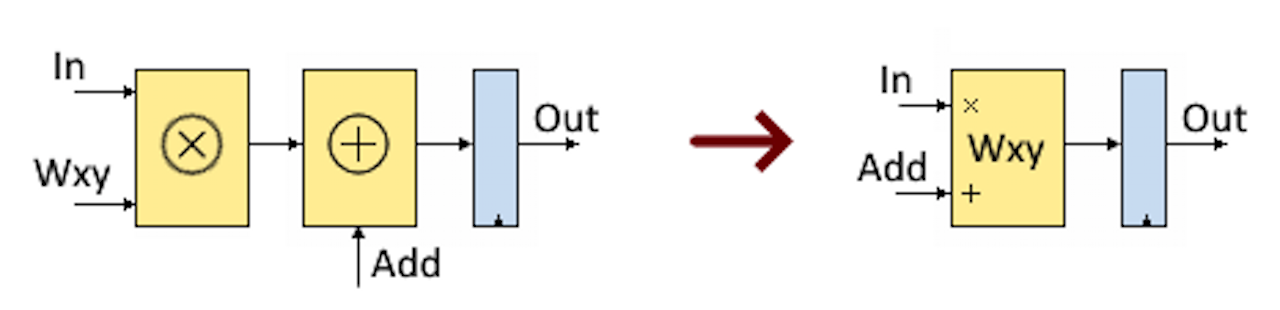
\includegraphics[width=0.65\textwidth]{MulAddReg10.png}
	\captionsource{Mul-Add register.}{\href{https://qengineering.eu/google-corals-tpu-explained.html}{Q-engineering}}
	\label{fig:mul-add-register}
\end{figure}
%
%
%\break For the sake of simplicity, no additional propagation time fixing registers have
%been added. With the formula of the neural node in mind, it is now relatively
%easy to design such a neuron with a few mul-add cells. Below the schematic for a
%three input neuron.
%
\begin{figure}[htb]
	\centering
	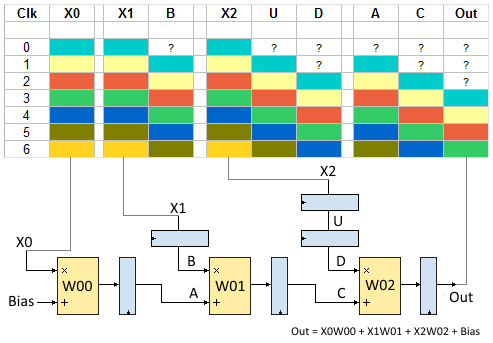
\includegraphics[width=0.75\textwidth]{Neuron.png}
	\captionsource{Schematic for a
three input neuron.}{\href{https://qengineering.eu/google-corals-tpu-explained.html}{Q-engineering}}
	\label{fig:3-input-neuron}
\end{figure}
%
%
Are necessary many important clarifications about the input registers
\texttt{X1} and \texttt{X2} displayed in figure (\ref{fig:3-input-neuron}). They
generate a delay line in the \emph{mul-add} chain, thus can permit to correct
synchronize. Considering the second cell \emph{mul-add} who sum the output from
previous cell (signal \texttt{A}) retarded by one clock cycle. Consequently also
the multiplication between the value in register \texttt{X1} and weight value
must be delayed the same amount of time. The schema reported in figure
(\ref{fig:3-input-neuron}) shows for each colour that represent the vector of
input \texttt{$[X0, X1, X2]$} while the input \texttt{A} and \texttt{B},
represented by lines straight, maintains always same colour. This means that
they appear simultaneous, i.e. are synchronised. The same must be valid for
input \texttt{C} and \texttt{D}.
%
\subsection{Systolic array}
\label{ssec:hard-systolic-array}
Starting from structure, just examined, is quite easy extend it to other
neurons, taking into account that every single input is connected with all
neurons in the next layer, as shows in figure
(\ref{fig:systolic-array-edge-tpu}).
%
\begin{figure}[htb]
	\centering
	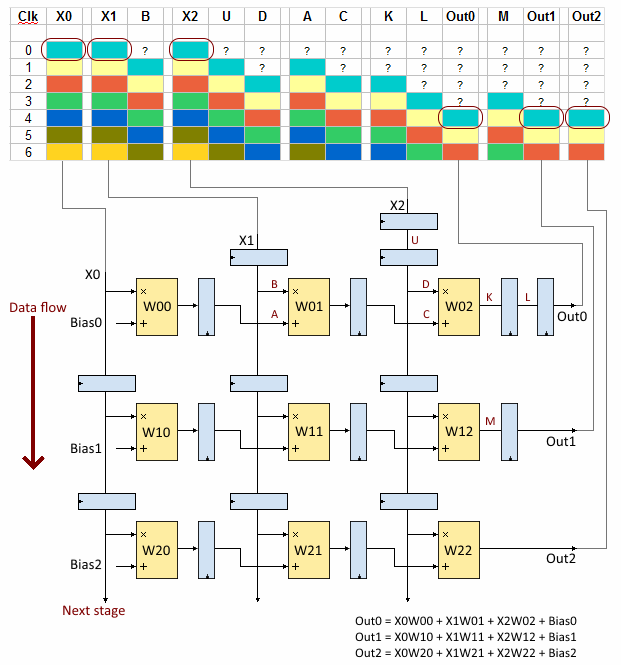
\includegraphics[width=0.75\textwidth]{Systolic-Array.png}
	\captionsource{Systolic Array Edge TPU.}{\href{https://qengineering.eu/google-corals-tpu-explained.html}{Q-engineering}}
	\label{fig:systolic-array-edge-tpu}
\end{figure}
%
%
The adoption of this solution, called systolic array, permits to have an
increment of speed in parallel calculation. 
Since the propagation time remains unchanged for an spread of systolic array in
depth or width, while only the latency time grows up this represent the solution
widely used for neural network hardware.
%
%The sizes of the systolic array in the Edge TPU are not known yet. The first TPU
%Google uses in its datacenter contains 256 x 256 \emph{mul-add} cells. Running at 700
%MHz it can theoretical performs 256 x 256 x 700.000.000 = 46 trillion \emph{mul-adds}
%per second. Or if you look to individual operations 92 trillion (92 TOPS).
%However, this impressive figure is purely theoretical. In practice, there are
%some factors that slow performance.
%
%The systolic array is made up of hardware. This means that it has fixed
%dimensions. Therefore, the input and output vectors also have fixed dimensions.
%However, the numbers of neurons per layer are determined by the design and are
%certainly not constant. If the number is smaller than the size of the array, it
%is, of course, possible to expand an input vector with leading zeros, so that
%the dimension equals the array size. The same technique can be applied to an
%oversized output vector.
%
%If the input vector contains more elements than the width of the systolic array,
%the entire arithmetic calculation must be performed in more than one call. To
%this end, the input vector is cut into a series of smaller vectors that match
%the width of the series. They are then processed one after the other. The
%intermediate results must be stored in a buffer. These values must be added
%after completion of all the systolic calls. Note that not only the input vector
%is split into smaller parts, but all weights used in the multiplication must be
%updated according to the formula's processing section. This may require a
%massive memory transfer. Below an example of a systolic array with only four
%inputs processing a vector of size 12.
%
%
%
%Looking at Google's schematic overview of the TPU, these output buffers and
%accumulators are drawn at the bottom. (In their diagram, the output is at the
%bottom instead of the right as on our drawing).
%Google TPU detail
%
% 
%Buffers have also been placed on the input vector side in the diagram above.
%They act as a first-in-first-out buffer, a FIFO. This guarantees continuous
%input of the systolic array with input values. It may also have some rotating
%operations, which increases the performance of CNN networks. It is unclear
%whether Google uses this method here. 
%
%
\subsection{Activation unit}
\label{ssec:activation-unit}
Once the output is available, it is sent to the activation unit. This module
within the Edge TPU applies the activation function to the output. It is
hardwired. In other words, you cannot alter the function, it works like a ROM.
Probably it is a ReLU function as it is nowadays the most used activation
function and it is very easy to implement in hardware.\cite{TPU:explained}
%
%
% TPU versus Edge TPU. The Google's Edge TPU is a much smaller device than the
% TPUs that Google uses in its data centers. Below the PCB with the original TPU
% and the Edge TPU on the same scale. TPU vs Edge TPU It is obvious that such a
% small device cannot have the same functions as its much larger ancestor. The
% floor plan on the die does not allow this to happen. Nor can the systolic
% array have the $256 \times 256$ dimension as in the original TPU. Google has
% so far not revealed the measures in the Edge, but a well-founded estimate is
% $64 \times 64$ with a clock of $480 \si{\mega\hertz}$, resulting in 4 TOPS.
% Memory is also an issue. In the original chip, it takes around $29\%$ of the
% total floor plan. It is impossible that the same amount can be found on the
% Edge TPU die. Moreover, the chip is very energy efficient. It requires no
% cooling. This means that almost certainly all the buffering is outside the
% chip. It leaves only a simple transfer of input vectors, output vectors and
% weights to the chip.	
% Practice.

    \chapter{Software}
\label{chap:software}
%
% preface chapter
\lettrine[lines=3]{T}{his} chapter describes the software developed for the
hardware described in the chapter \ref{chap:hardware}. The choice to use the Qt
framework guarantees the portability to garntiee cross-platform support, as well
as the graphical interface and high data performance the feature of compiled
languages.  The software is divided into two programs capable of communicating
with each other: the first works on Raspberry Pi and allows the user to
interface easily with the FLir thermal camera and with the Raspicam camera. It
also acts as a TCP server for sending the images shot to connected devices. The
second part is a client program that receives the data sent by the main device,
and allows the analysis of the image through machine learning on dedicated
hardware.
%
% input files
%
\section{Signals \& Slots}
\label{ref:soft-signal-slot}
In the project extensive use was made of the Signal and Slot mechanism, this to
allow communication between the objects in the code. Signals and slots are used
for communication between objects. The signals and slots mechanism is a central
feature of Qt and probably the part that differs most from the features provided
by other frameworks. Signals and slots are made possible by Qt's meta-object
system.\cite{Qt:signal-slot}

\subsection{Introduction}
\label{ssec:soft-intro}
In GUI programming, when we change one widget, we often want another widget to
be notified. More generally, we want objects of any kind to be able to
communicate with one another.

Other toolkits achieve this kind of communication using callbacks. A callback is
a pointer to a function, so if you want a processing function to notify you
about some event you pass a pointer to another function (the callback) to the
processing function. The processing function then calls the callback when
appropriate. While successful frameworks using this method do exist, callbacks
can be unintuitive and may suffer from problems in ensuring the type-correctness
of callback arguments.\cite{Qt:signal-slot}

\subsection{Signals and Slots}
\label{ssec:soft-sig-solt-detail}
In Qt, we have an alternative to the callback technique: We use signals and
slots. A signal is emitted when a particular event occurs. Qt's widgets have
many predefined signals, but we can always subclass widgets to add our own
signals to them. A slot is a function that is called in response to a particular
signal. Qt's widgets have many pre-defined slots, but it is common practice to
subclass widgets and add your own slots so that you can handle the signals that
you are interested in. 
%
%
\begin{figure}[htb]
	\centering
	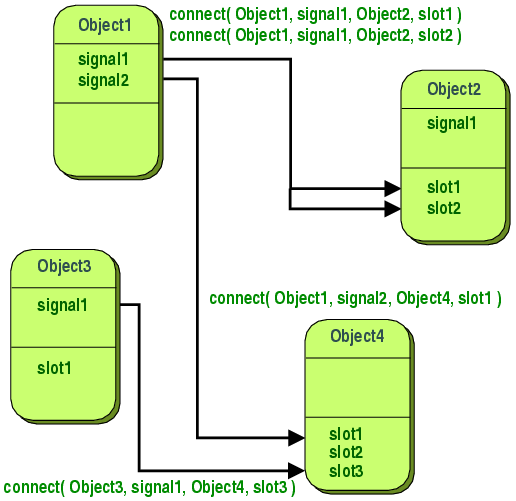
\includegraphics[width=0.65\textwidth]{abstract-connections.png}
	\caption{Signal and Slot scheme.}
	\label{fig:software-signal-slots-scheme}
\end{figure}
%
The signals and slots mechanism is type safe: The signature of a signal must
match the signature of the receiving slot. (In fact a slot may have a shorter
signature than the signal it receives because it can ignore extra arguments.)
Since the signatures are compatible, the compiler can help us detect type
mismatches when using the function pointer-based syntax. The string-based SIGNAL
and SLOT syntax will detect type mismatches at runtime. Signals and slots are
loosely coupled: A class which emits a signal neither knows nor cares which
slots receive the signal. Qt's signals and slots mechanism ensures that if you
connect a signal to a slot, the slot will be called with the signal's parameters
at the right time. Signals and slots can take any number of arguments of any
type. They are completely type safe.

All classes that inherit from QObject or one of its subclasses (e.g., QWidget)
can contain signals and slots. Signals are emitted by objects when they change
their state in a way that may be interesting to other objects. This is all the
object does to communicate. It does not know or care whether anything is
receiving the signals it emits. This is true information encapsulation, and
ensures that the object can be used as a software component.

Slots can be used for receiving signals, but they are also normal member
functions. Just as an object does not know if anything receives its signals, a
slot does not know if it has any signals connected to it. This ensures that
truly independent components can be created with Qt.

You can connect as many signals as you want to a single slot, and a signal can
be connected to as many slots as you need. It is even possible to connect a
signal directly to another signal. (This will emit the second signal immediately
whenever the first is emitted.)

Together, signals and slots make up a powerful component programming mechanism.\cite{Qt:signal-slot}

\subsection{Signals}
\label{ssec:soft-signal}
Signals are emitted by an object when its internal state has changed in some way
that might be interesting to the object's client or owner. Signals are public
access functions and can be emitted from anywhere, but we recommend to only emit
them from the class that defines the signal and its subclasses.

When a signal is emitted, the slots connected to it are usually executed
immediately, just like a normal function call. When this happens, the signals
and slots mechanism is totally independent of any GUI event loop. Execution of
the code following the emit statement will occur once all slots have returned.
The situation is slightly different when using queued connections; in such a
case, the code following the \textbf{\texttt{emit}} keyword will continue
immediately, and the slots will be executed later.

If several slots are connected to one signal, the slots will be executed one
after the other, in the order they have been connected, when the signal is
emitted.

Signals are automatically generated by the \emph{moc} and must not be implemented in
the \texttt{.cpp} file. They can never have return types (i.e. use void).\cite{Qt:signal-slot}

\subsection{Slots}
\label{ssec:soft-slots}
A slot is called when a signal connected to it is emitted. Slots are normal C++
functions and can be called normally; their only special feature is that signals
can be connected to them.

Since slots are normal member functions, they follow the normal C++ rules when
called directly. However, as slots, they can be invoked by any component,
regardless of its access level, via a signal-slot connection. This means that a
signal emitted from an instance of an arbitrary class can cause a private slot
to be invoked in an instance of an unrelated class.

Compared to callbacks, signals and slots are slightly slower because of the
increased flexibility they provide, although the difference for real
applications is insignificant. In general, emitting a signal that is connected
to some slots, is approximately ten times slower than calling the receivers
directly, with non-virtual function calls. This is the overhead required to
locate the connection object, to safely iterate over all connections (i.e.
checking that subsequent receivers have not been destroyed during the emission),
and to marshall any parameters in a generic fashion. While ten non-virtual
function calls may sound like a lot, it's much less overhead than any
\texttt{new} or \texttt{delete} operation, for example. As soon as you perform a
string, vector or list operation that behind the scene requires \texttt{new} or
\texttt{delete}, the signals and slots overhead is only responsible for a very
small proportion of the complete function call costs. The same is true whenever
you do a system call in a slot; or indirectly call more than ten functions. The
simplicity and flexibility of the signals and slots mechanism is well worth the
overhead, which your users won't even notice.\cite{Qt:signal-slot}

%
% introduction
\section{Interface}
\label{sec:raspberry-software}
As anticipated, the software run on the Raspberry Pi is made following the
paradigm of object-oriented programming. Made in C++/Qt making extensive use
of the proprietary classes of the framework and the Standard Template Library
(STL). This program has some dependencies with regard to the thermal camera
drivers supplied by the manufacturer and are 32-bit, since the Raspberry Pi 3,
described in \ref{sec:raspi3}, is equipped with a 32-bit ARM Cortex-A53
processor. These allow total control of the camera. The second dependency is the
Raspicam library which allows the interface with the RGB camera allowing the
image acquisition.
%
\begin{figure}[htb]
	\centering
	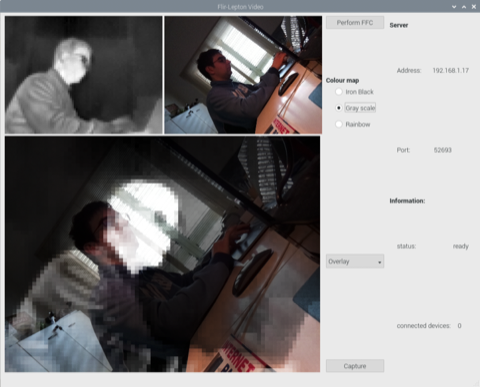
\includegraphics[width=0.65\textwidth]{grayscale.png}
	\caption{User interface run on Raspberry Pi 3b.}
	\label{fig:software-main-ui}
\end{figure}
%
% interface
Continuing a user interface has been created through the use of widgets, this is
divided into three areas. The first area shows the video streams acquired
separately in two labels, the third larger label shows the two streams mixed
through filters made available as default the overlay filter is used. It was
preferred not to perform a match of the images with pixel-by-pixel recalculation
for two reasons: the first due to the high difference in size of the sensors as
that of the thermal camera is $80 \times 60$ pixels while the Raspicam is $3280
\times 2464$ pixels. Furthermore motivation is due to not aggravate the 
computational load on the CPU.
The second area provides some controls for the user, in fact it is
possible to save thermal images on files during the acquisition. you can change
the heat map applied to the image on the fly by choosing from three different
possibilities, in the figure you can observe the result. 
Finally, it is possible to modify the mixing filter, also on the fly, of the
video streams to obtain different effects to improve visibility or to increase
details.
The last section of the user interface shows the information relating
to the TCP socket used for sending the video stream to other devices.
%
% image ui
\begin{figure}[htb]
    \centering
    \subfloat[][\emph{lava}.\label{subfig:lava-map}]
        {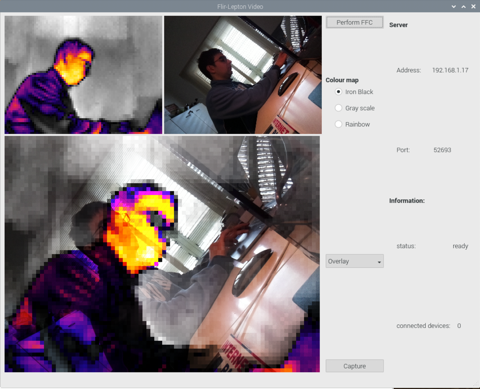
\includegraphics[width=.30\textwidth]{lava.png}} \quad
    \subfloat[][\emph{grayscale}.\label{subfig:grayscale-map}]
        {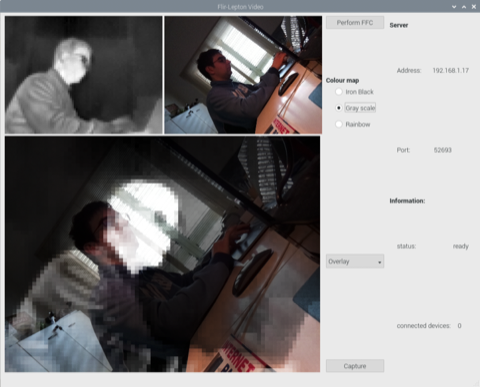
\includegraphics[width=.30\textwidth]{grayscale.png}} \quad
    \subfloat[][\emph{rainbow}.\label{subfig:rainbow-map}]
        {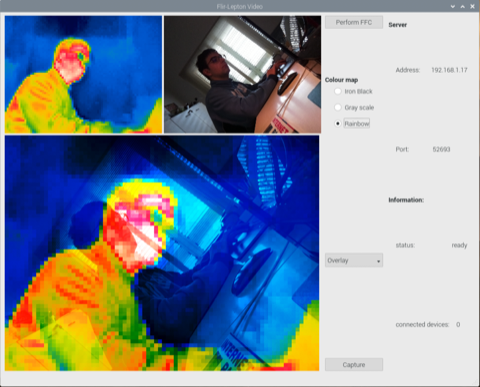
\includegraphics[width=.30\textwidth]{rainbow.png}}
    \caption{Result colourization applied to thermal camera data.}
    \label{fig:reuslt-maps}
\end{figure}
%
% software analysis 
\subsection{Software Analysis}
\label{ssec:raspberry-softw-analysis}
The user interface is run on the main thread, in order to maximize the
performance of the executed code the image acquisition operation is performed in
the secondary thread. Thanks to the use of the signal and slot system of Qt, 
introduced before in (\ref{ref:soft-signal-slot}), it is possible to update the 
labels without blocks typical of multi-threaded programming. 
The difficulty of concurrent programming usually consists in
synchronizing the access to resources by different threads that act in
competition on the same resources. Having two or more threads accessing the same
data simultaneously can lead to unexpected and unwanted results. 
In fact, without the application of particular programming techniques, it is not
possible to predict in a deterministic way, at the time of execution, when that
specific thread will be executed: their progression depends on the priorities
decided by the scheduler of the operating system and not by the programmer. 
In fact, multiple threads can access the same variable and modify its content or
value. Therefore, synchronization techniques such as mutual exclusion are used
to solve the problem. As a result, ideally a thread should execute code as
independent of the rest of the program as possible. Furthermore, errors in
synchronization between threads are often very difficult to detect because their
occurrence essentially depends on the environment in which the program is run.
The synchronization of one thread with another is normally necessary to allow
them to communicate with each other and to return the results of a function to
the main process; it is normally done through \emph{mutex}\cite{wiki:thread}.
Analysing the code of the thread that takes care of acquiring the images we can 
see that it proceeds without mutex\footnote{The mutex class is a synchronization
primitive that can be used to protect shared data from being simultaneously
accessed by multiple threads.}, but uses the signal and slot system as mentioned
before.
%
% code list
\inputminted[frame=lines,framesep=2mm, linenos=true, autogobble, breaklines=true, fontsize=\scriptsize, firstline=36, lastline=100]{c++}{software/code/leptonthread.cpp} 
\captionof{listing}{Infinite loop thread cameras.\label{lst:rasp-leptonthread}}
%
\pagebreak
Going to analyse in detail the infinite loop, reported in the
listing (\ref{lst:rasp-leptonthread}), executed in a thread other than the main
one that manages only the main interface, it can be observed that:
\begin{itemize}
\item (line 37--56) When the function starts, an instance of the \texttt{QImage}
type object is instantiated to contain the image acquired during the cycle. The
parameters of the frame size are provided and the color space this allows to
increase the speed of the cycle as it will not be cyclically cancelled and
reallocated the same, but will be reused. The communication with the thermal
camera is opened via the SPI port if the cycle is not started or if the
communication is interrupted the communication is closed.
% code list
%\begin{minipage}{\linewidth}
%\centering
%\inputminted[bgcolor=bg,frame=lines,framesep=2mm, linenos=true, autogobble, breaklines=true, fontsize=\scriptsize, firstline=36, lastline=61]{c++}{software/code/leptonthread.cpp} 
%\captionof{listing}{Data acquisition from SPI.}
%\label{lst:rasp-leptonthread-data} 
%\end{minipage}
%
\item (line 66--78) The main cycle is to acquire data from the saved camera
registers, as the order is MSB\footnote{MSB can also stand for "most significant
byte". \emph{Big-endian processor}: When data is loaded into a multi-byte
register, the first byte (with the lowest address) is the most significant byte
of the data.\cite{56322}}, reversed in according to LSB\footnote{LSB can also
stand for "least significant byte". \emph{Little-endian processor}: When data is
loaded into a multi-byte register, the first byte (with the lowest address) is
the least significant byte of the data.\cite{56322}}. The values are then scaled
to obtain a consistent representation of the hot and cold areas. Then the color
map is applied to color the raw data obtained from the scaling process described
above.
%% code list
%\begin{minipage}{\linewidth}
%\centering 
%\inputminted[bgcolor=bg,frame=lines,framesep=2mm, linenos=true, autogobble, breaklines=true, fontsize=\scriptsize, firstline=79, lastline=108]{c++}{software/code/leptonthread.cpp} 
%\captionof{listing}{Flip the MSB and LSB and colouration.} 
%\label{lst:rasp-leptonthread-MSB-LSB} 
%\end{minipage}\linebreak
%%
\item (line 79--97) Finally, signals are output for the coloured thermal image,
for the RGB image acquired by the Raspicam library and passed through the slot
and the last resulting from mixing of previous two depend on effect of selected
in UI interface.
%% code list
%\begin{minipage}{\linewidth}
%\centering 
%\inputminted[bgcolor=bg,frame=lines,framesep=2mm, linenos=true, autogobble, breaklines=true, fontsize=\scriptsize, firstline=36, lastline=117]{c++}{software/code/leptonthread.cpp} 
%\captionof{listing}{Infinite loop thread cameras.} 
%\label{lst:rasp-leptonthread} 
%\end{minipage}
\end{itemize}
As can be seen, the cycle proceeds without mutuals or blocking conditions, in
fact, as previously described, it is possible to change the color map or the
mixing tool on the fly.
%
% analysing comunication
% description socket tcp
\newpage
\section{Communication systems}
\label{sec:software-TCPSocket}
In digital data communications, wiring together two or more devices is one of
the first steps in establishing a network. As well as this hardware requirement,
software must also be addressed. The Open System Interconnection (OSI) model
proposed by the International Organization for Standardization (ISO) is a
standard way to structure communication software that is applicable to any
network. The model has been standardized by ISO and International
Telecommunication Union (ITU) Telecommunication Standardization Sector (ITU-T)
which is the organization coordinating standards for telecommunications. 
The
communication is based on low-level message passing between the communicating
systems.
\begin{itemize}
\item A wants to communicate with B; 
\item A builds a message addressing B; 
\item A executes a call to the communication module to send the message to B.
\end{itemize}
Of course, A and B need to speak the same language, i.e., they need to agree on the meaning
of the bits being sent. The protocols define the rules for communication. 
When
data is exchanged through a computer network, the system rules are called a
network protocol. A protocol must define the syntax, semantics, and timing of
communication (i.e. how, what and when); the specified behaviour is typically
independent of how it is to be implemented. Syntax: refers to the structure or
the format of the data. Semantics: the way in which the bit patterns are
interpreted. Timing: specify when the data can be sent and how fast it will be.
Another term is synchronization.
The communication between two nodes of a network occurs by sending messages. a
message is broken down into a sequence of packets, and each packet is
transmitted individually.
The structure includes some control bits at the beginning of the message called
\emph{header} and at the end called \emph{footer}.
the control bits can contain information such as: the sending node of the
packet, the recipient node of the package, package length information,
information that allows you to verify the correctness of the package. \cite{mandrioli2008informatica}
%
% %TODO Insert image
% image 
%
\subsection{Architecture}
\label{ssec:soft-client-server}
Client/server architectures are based on the functional division of IT
applications into two categories. Few computers act as servers, run a particular
program that allows the computer to receive requests and send replies.
As shows in figure (\ref{fig:client-server architecture}).\hfill \break
The clients, on the other hand, run a program that allows them to send requests and
receive replies. Client/server applications are two-level architectures, that
is, the first level is the client and the second level is the server. The
interaction protocols between client and server are quite simple. among the
advantages of client/server architectures we have the simplicity of
construction and the possibility of having easy-to-use clients.\\ 
Disadvantages include the risk of overloading the computer acting as a server 
and the communication channel with which the server is connected to the network.\cite{mandrioli2008informatica}\hfill \break
%
%
\begin{figure}[ht]
	\centering
	\resizebox{0.65\textwidth}{!}{\begin{tikzpicture}[block/.style={draw,minimum width=2cm,minimum height=1cm}, font=\sffamily] 
\node[block](C) {Client}; 
\node[block,right=9cm of C](S) {Server}; 
\draw[-latex] (C.15) -- (S.165)	node[midway,above]{Request}; 
\draw[-latex] (S.195) -- (C.-15) node[midway,below]{Response}; 
\end{tikzpicture}}
	\caption{Two level client/server architecture} 
	\label{fig:client-server architecture}
\end{figure}
%
\newline In the Internet protocol suite there is also the Transmission Control Protocol
(TCP). It is the complement of the Internet Protocol, yielding the well known
TCP/IP. TCP provides reliable, ordered, and error-checked delivery of the
messages between applications on an IP network. The most used internet
applications, i.e. the World Wide Web, e-mail, file transfer, rely on TCP.
%
\subsection{Server implementation}
\label{ssec:soft-rasp-server}
In our case, it implements \texttt{QTcpSocket} network communication.  So, there
is a server service in main program shows in figure
(\ref{fig:software-socket-server}). While there is a client application deepened
later in section (\ref{sec:software-coral-intro}). Server application has
\texttt{QTcpSocket} and it listens to some port, in our case $52693$.
 Client has \texttt{QTcpSocket}, but has not connected to the server yet:\linebreak
%
%
\begin{figure}[!ht]
	\centering
	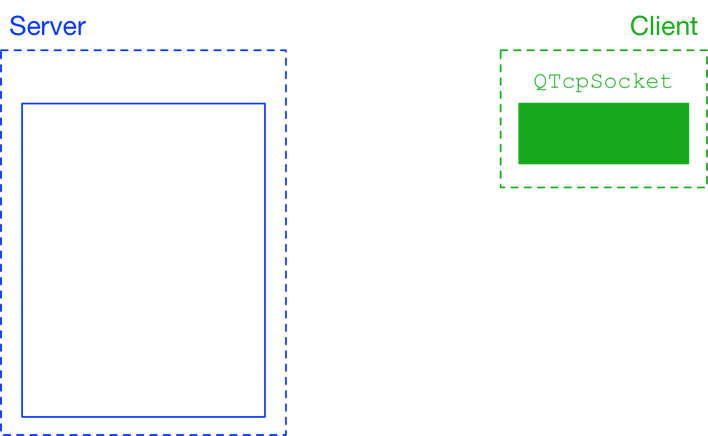
\includegraphics[width=0.7\textwidth]{qtcpserver-qtcpsocket.png}
	\caption{Interface client server \texttt{QTcpSocket}.}
	\label{fig:software-socket-server}
\end{figure}
%
\\When client connects to server, a \texttt{QTcpSocket} is created on the server’s
side, through which server and client can talk to each other and start send
message, shows in figure (\ref{fig:software-socket-server-client}).
%
%
\begin{figure}[htb]
	\centering
	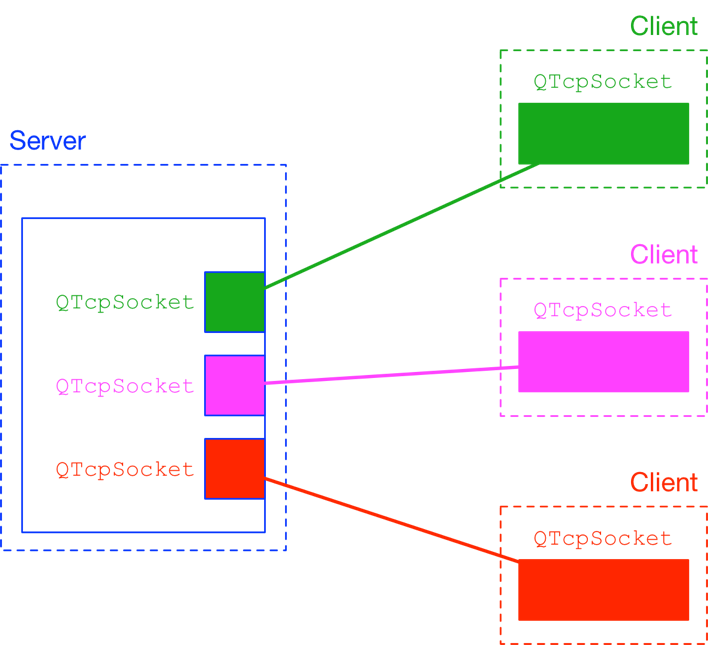
\includegraphics[width=0.55\textwidth]{qtcpserver-qtcpsocket-clients.png}
	\caption{Connection between server-clients.}
	\label{fig:software-socket-server-client}
\end{figure}
%
In particular, we observe the function reported in (\ref{lst:rasp-code-thread})
implemented in server application which sends the image just captured by the RGB
camera to the server to be  encapsulated in the message before send. 
In the function it is possible to observe the presence of a mutex which is 
locked to protect the resource and avoid overwriting through function calls.
The frame, i.e. the resource, is converted and stored in buffer before
sending.\\ 
Upon exiting the function body, the mutex is unlocked, thus giving free
access to resources again.
% code list
\begin{listing}[ht]
\inputminted[frame=lines,framesep=2mm, linenos=true, autogobble, breaklines=true, fontsize=\scriptsize, firstline=84, lastline=95]{c++}{software/code/mainwindow.cpp} 
\caption{Particular report function sending image.} 
\label{lst:rasp-code-thread} 
\end{listing}

%
% introduction
\section{Client}
\label{sec:software-coral-intro}
The software that acts as a client on the Coral dev-board, presented in chapter
\ref{}, created by Google is based on the same Qt framework previously
introduced in order to guarantee portability and reliability of the code. This,
remember, has an ARM Cortex-A53 processor, but unlike the one mounted on
Raspberry it executes 64-bit code and takes advantage of the new armv8
architecture with a significant performance gain. This difference arises from
the execution of Machine Learning operations supported by the TPU, described in
detail in section \ref{}.
%
% interface
As seen for the main program, here too we find a main interface executed in the
main thread. The simplest interface is divided into two areas: the first one
where it is possible to observe the flow of images coming from the TCP socket
analyzed later. The second, on the other hand, offers the possibility of
connecting to the TCP socket by entering the address and port of the machine on
which the server is run, which is listening for possible connection requests.
Once the connection between server and client is established, the label is
updated with the images received.
%
% software analysis
\subsection{Software Analysis}
\label{ssec:software-coral-analysis}
To avoid blockages and unpleasant delays in receiving images from the TCP
socket, multi-thread programming was used. In fact, as previously described, the
interface managed by QWidget is run on the main thread. If the connection is
stable, the thread starts which allows reception in a queue waiting to leave.\\ 
On the other hand, this is prepared when the class is instantiated within the
main function. Since this infinite cycle is the critical factor, we analyse its
structure in detail below.
%
% code list
\begin{listing}[ht] 
\inputminted[frame=lines,framesep=2mm, linenos=true, autogobble, breaklines=true, fontsize=\scriptsize, firstline=12, lastline=26]{c++}{software/code/streamerthread.cpp} 
\caption{Particular report function sending image.} 
\label{lst:coral-client-code} 
\end{listing}
%
\\As you can see in the function code, shown in Listing
(\ref{lst:coral-client-code}), we observe the instance of the \texttt{socket}
member object of the \texttt{QTcpSocket} class type. 
By starting the connection, the server. 
The critical section from the \emph{while loop} is protected by a mutex,
highlighted by the \texttt{QMutexLocker} class, a mutex indicates a
process of synchronization between concurrent processes or threads, with which
multiple parallel tasks are prevented from simultaneously accessing 
data in memory or other resources subject to race condition.\cite{wiki:mutex} 
Locking and unlocking a \texttt{QMutex} in complex functions and statements or
in exception handling code is error-prone.
\texttt{QMutexLocker} can be used in such situations to ensure that the state of the
mutex is always well-defined. \texttt{QMutexLocker} should be created within a
function where a \texttt{QMutex} needs to be locked. The mutex is locked when
\texttt{QMutexLocker} is created. If locked, the mutex will be unlocked when
the \texttt{QMutexLocker} is destroyed.
Using \texttt{QMutexLocker} greatly simplifies the code, and makes it more
readable.\cite{Qt:QMutexclass}
The buffer is filled with reading from the socket and before putting the signal
to update the image in the interface a small interval of time is waited to
guarantee the complete reception of the image.
Before updating the label on the dashboard, filter the image to verify that it
is consistent and different from an empty or corrupt image, shows in listing
(\ref{lst:coral-ui-code}). 
If this occurs, the function is immediately exited to
avoid viewing an image being ready to receive a new image. 
%
% code list
\begin{listing}[ht] 
\inputminted[frame=lines,framesep=2mm, linenos=true, autogobble, breaklines=true, fontsize=\scriptsize, firstline=88, lastline=100]{c++}{software/code/tcpclient.cpp} 
\caption{Implantation filter.} 
\label{lst:coral-ui-code} 
\end{listing}
%
% cnn part
\subsection{CNN-PART-TPU-INFERENCE}
%TODO
...

    \chapter{Neural Networks}
\label{chap:neuralnetworks}
%
% preface chapter
\lettrine[lines=3]{D}{eep} Learning has exploded to the present day because it
has become accessible to the general public. Often its contribution is
noticeable in intelligent systems as assistants and interpreters of natural
language and prototypes of self-driving vehicle systems. In this document, we
try to provide a thorough investigation of deep learning in its applications and
mechanisms. In particular, as a categorical state of the art collection in
research on deep learning. An impetus in deep learning technologies was imparted
by Google in 2015 thanks to TensorFlow. TensorFlow supports computation on
multiple CPUs and GPUs, with optional CUDA and SYCL extensions. In addition,
TensorFlow Lite is designed for mobile and embedded machine learning, and
provides an Android Neural Networks API.\cite{article}
% 
% 
\section{Introduction}
\label{sec:intro}
In this era, a large amount of structured and unstructured data became
available. \textbf{Machine Learning} (\textbf{ML}) has evolved as a branch of
artificial intelligence: it envisages the development of self-learning
algorithms, which are capable of acquiring knowledge from data with the aim of
making predictions. Instead of requiring a human presence who manually enact the
rules and build models for the analysis of large amounts of data, machine
learning offers a more efficient alternative to capture the knowledge in the
data. Machine learning aims to gradually improve the performance of forecasting
models and to make data driven decisions. In this section we will examine the
three different types of machine learning: \emph{supervised learning},
\emph{unsupervised learning} and \emph{reinforcement learning}. Where we will
show the fundamental differences between these types of
learning.\cite{raschka2016machine}
%
\subsection{Supervised learning}
\label{subsec:supervised-learnig}
The main purpose of supervised learning is to derive a model from  training
data, which allows us to make predictions for data that are not available or
future. Here, the term ``supervision" refers to the fact that the output signal
labels  of the sample sets are already known. A supervised learning task, which
is based on discrete class labels, is also  called a classification task, in
figure \ref{fig:supervised-learning-scheme} it  is possible to observe a process
diagram. Another supervised learning subcategory is regression, whose resulting
signal is a continuous value. Classification is a sub-category of supervised
learning, which has the goal to provide class category labels for new instances,
based on observations made in the past.

These labels are discrete, unordered values that can be considered as belonging
to a group of instances. However, the set of class labels does not necessarily
have to be a binary nature. The predictive model identified by a supervised
learning algorithm can consider each class label that is present in the learning
dataset of a new instance, which is not labelled. A typical example of
\emph{multi-class classification} is the recognition of hand-written
text.\cite{raschka2016machine}
%
\begin{figure}[!h]
\centering
%\draw [help lines] (0,0) grid (8,8);
\resizebox{0.65\textwidth}{!}{\begin{tikzpicture}[auto,>=latex']
%\draw [help lines] (0,0) grid (8,8);
\tikzset{
	boxA/.style={
  		rectangle,
  		inner sep=0pt,
  		text width=25mm,
  		align=center,
  		draw=black,
  		fill=airforceblue,
  		minimum height = 10mm
  	},
  	boxB/.style={
  		rectangle,
  		inner sep=0pt,
  		text width=25mm,
  		align=center,
  		draw=black,
  		fill=amber,
  		minimum height = 10mm
  	},
  	boxB1/.style={
  		rectangle,
  		inner sep=0pt,
  		text width=25mm,
  		align=center,
  		draw=black,
  		fill=amber!30,
  		minimum height = 10mm
  	},
  	boxC/.style={
  		rectangle,
  		inner sep=0pt,
  		text width=25mm,
  		align=center,
  		draw=black,
  		fill=light-gray,
  		minimum height = 10mm
  	},
  }

\node (a) [boxC, align=center] at (1,1) {New data};
\node (b) [boxC, align=center] at (5,1) {Predicitve\\ model};
\node (c) [boxC, align=center] at (9,1) {Prediction};
\node (d) [boxA, align=center] at (5,3) {Alogrithm\\ DNN};
\node (e) [boxB, align=center] at (5,5) {Dataset};
\node (e1) [boxB1, align=center] at (6,5.85) {Label};
\draw [->] (a) -- (b);
\draw [->] (b) -- (c);
\draw [->] (d) -- (b); 
\draw [->] (e) -- (d); 
\end{tikzpicture}}
\caption{supervised learning scheme} 
\label{fig:supervised-learning-scheme}
\end{figure}
%
\subsection{Reinforcement learnig}
\label{subsec:reinforcement-learnig}
Another type of machine learning is reinforcement learning. Here, the goal is to
develop a system (\emph{agent}) for people to improve their performance. In
order to do so, that system is based on interactions with  the environment.
Since information relating to the current state of the environment include also
a \emph{reward} signal, we can consider strengthening learning as an example of
supervised learning. However, this feedback is not the correct label or the true
value of truth, but it represents the quality of the measurement of the 
performance measured by the reward function. \hfill \break
Through interaction with the environment, an agent can then use reinforcement
learning to learn a series of actions, which maximize this reward through a
trial-and-error exploratory approach or deliberative
planning.\cite{raschka2016machine}
%
\begin{figure}[!h]
\centering
\begin{tikzpicture}[>=latex]
 %\draw [help lines] (0,0) grid [step=0.5] (8,4);
 \draw (0.5,0) rectangle ++(3cm, 1.5cm);
 \draw (4.5,2.5) rectangle ++(3cm,1.5cm);
 %\node [draw] (1.5,2) {Agent};
 \coordinate [label={[font=\small]center:Agent}] (A) at (2,0.75);
 \coordinate [label={[font=\small]center:Envoiroment}] (E) at (6,3.25);
 \draw [-, ultra thick] (3.5,0.75) -- (6,0.75);
 \draw [->, ultra thick] (6,.75) -- (6,2.5);
 \coordinate [label={[font=\small]center:State}] (S) at (6.5,1.5);
 %
 \draw [-, ultra thick] (4.5,2.75) -- (3,2.75);
 \draw [->, ultra thick] (3,2.75) -- (3,1.5);
 \coordinate [label={[font=\small]center:Action}] (T) at (3.5,3);
 %
 \draw [-, ultra thick] (4.5,3.75) -- (1,3.75);
 \draw [->, ultra thick] (1,3.75) -- (1,1.5);
 \coordinate [label={[font=\small]center:Reward}] (R) at (1.75,3.5);
\end{tikzpicture} 
\caption{reinforcement learning scheme} 
\label{fig:reinforcement-learning-scheme}
\end{figure}
%
\subsection{Unsupervised learning}
\label{subsec:unsupervised-learning}
In supervised learning, we know in advance the correct answer when we describe
our model, while in reinforcement learning we define a measure, or reward, for
the specific actions performed by the agent. In unsupervised learning, on the
other hand, we are dealing with unlabelled data or data from the unknown
structure. Using unsupervised learning techniques, we are able to observe the
structure of our data, to extract meaningful information from them without being
able to rely on the guide nor a variable known relative result, nor a reward
function. Clustering is an exploratory technique of data analysis that allows us
to organize a series of information within meaningful groups (\emph{cluster})
without having any previous knowledge of memberships in such groups. Each
cluster that can be derived during the analysis defines a group of objects that
share a certain degree of similarity, but which are more dissimilar than the
objects present in the other clusters, which is why clustering is sometimes
called \emph{``unsupervised classification"}. Clustering is an excellent
technique for structuring information to identify meaningful relationships in
the data.\cite{raschka2016machine}
%
\begin{figure}[!h]
\centering
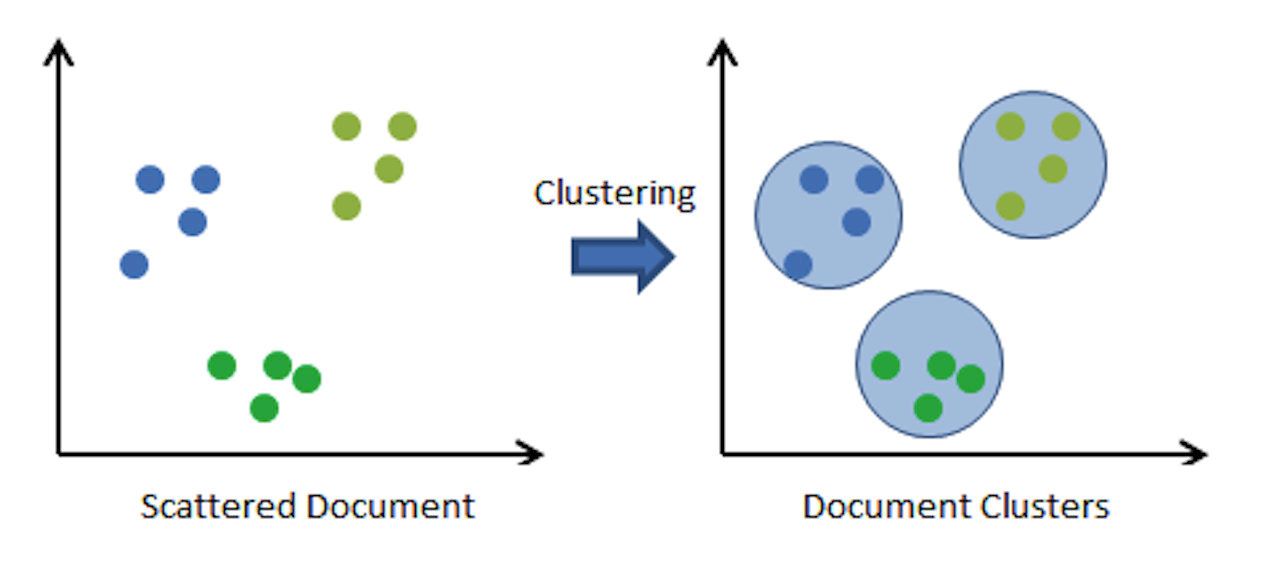
\includegraphics[width=0.70\textwidth]{cluster.jpg}
\caption{example of clustering}
\label{fig:unsupervised-learning-scheme}
\end{figure}

\section{Deep Learning for Object Detection}
\label{sec:nn-objectdetection}
Object detection is fundamental computer vision problem visual recognition other
than image classification, semantic segmentation. 
In particular object detection not only recognizes object categories but also
predicts the location of each object by a bounding box. 
On the other hand semantic segmentation aims to predict pixel-wise classifiers
to assign a specific category label to each pixel, thus providing an even richer
understanding of an image. 
However, in contrast to object detections, semantic segmentation does not
distinguish between multiple objects of the same category.\cite{wu2020recent}\\
Current state-of-the-art object detection systems are variants of the following
approach: hypothesize bounding boxes, re-sample pixels or features for each box,
and apply a high quality classifier.
Although accurate, these approaches have been too computationally intensive for
embedded systems and, even with high-end hardware, too slow for real-time or
near real-time applications. 
Often detection speed for these approaches is measured in seconds per frame, and
even the fastest high-accuracy detector, the basic Faster R-CNN, operates at
only $7$ frames per second (FPS). 
There have been a wide range of attempts to build faster detectors by attacking
each stage of the detection pipeline, but so far, significantly increased speed
comes only at the cost of significantly decreased detection
accuracy.\cite{liu2016ssd}
To derive a performance improvement translated into an increase in detection
speed with high precision ($58$ FPS with mAP $72.1\%$ on VOC2007 test, vs Faster
R-CNN $7$ FPS with mAP $73.2\%$ or YOLO $45$ FPS with mAP $63.4\%$). 
From this derives the elimination of the proposals of delimitation boxes and of
the subsequent phase of re-filling of the pixels or of the characteristics. 
Furthermore, the improvements introduced can be summarized in the use of a
convolution filter to predict the categories of objects and offsets in the
positions in the positioning of the panes, using separate predictors (filters)
for different aspect ratio detections, and applying these filters to multiple
features maps from the later stages of a network in order to perform detection
at multiple scales.
It is observed that with these modifications we can achieve high-accuracy
detection using relatively low resolution input and further increasing
processing speed. While these contributions may seem independently small, we
note that the resulting system improves accuracy on high-speed detection for
PASCAL VOC from $63.4\%$ mAP for YOLO to $72.1\%$ mAP for the network
used.\cite{liu2016ssd,Huang2016SpeedAccuracyTF}
So as to ensure stability and portability of the model The API TensorFlow Object
Detection is used, an open source framework based on TensorFlow which simplifies
the construction, training and implementation of object detection
Templates.\cite{objectdetectionAPI}
%
%
\begin{figure}[!h]
	\centering
	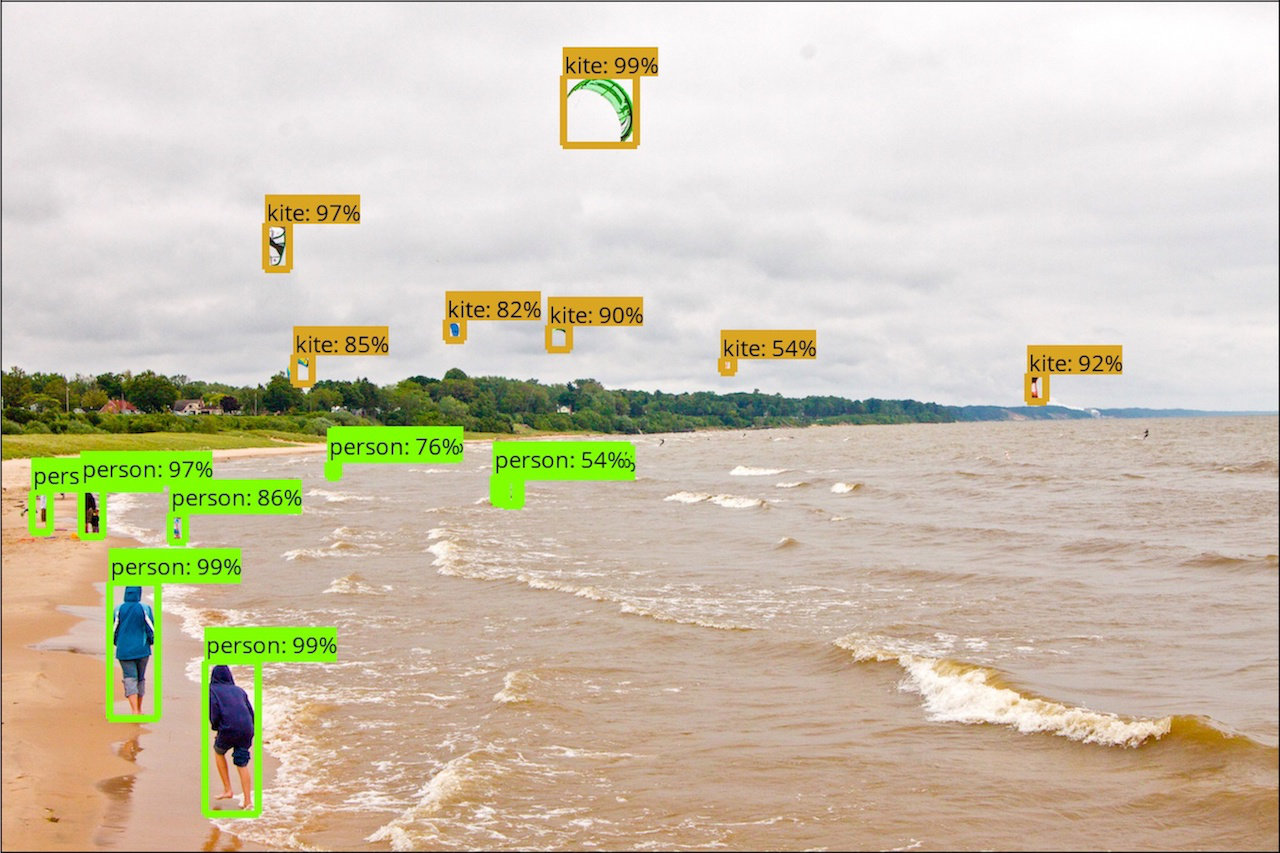
\includegraphics[width=0.75\textwidth]{kites_detections_output.jpg}
	\captionsource{example multiple object detection in a single image.}%
	{\href{https://github.com/tensorflow/models/tree/master/research/object_detection}{GitHub.com - TensorFlow}}
	\label{fig:kites-detections-output}
\end{figure}
%
%
\subsection{Single Shot Detector MobileNet}
\label{ssec:single-shot-detector}
The model of SSD is based on the idea that we want to detect the position of an 
object of interest, in addition to knowing which one is classified. 
To better comprehend let’s start from nomenclature: 
\begin{description}
\item[Single Shot] The localization and classification operation must be a single forward pass of the network.
\item[Multibox] Technique for bounding box regression.
\item[Detector] The neural network has the duty classifies those detected object.
\end{description}
%
The model \emph{SSD MobileNet} exploit four stages: the input layer for
importing the target image, the MobileNet base for extracting image features,
the SSD for classification regression and bounded box regression and the output
layer for exporting the detection result.\cite{Li_2018} 
The advantage of this net are speed and accuracy in detection task borrowed from
reduced compute complexity.
%
\begin{table}[htb]
	\centering
	\begin{tabular}{l c c c}
	\hline
		Model name								&Speed (ms)	& COCO mAP\footnotemark	& Outputs\\
		\hline
		ssd\_mobilenet\_v1\_coco					&	30		&	21		&	Boxes\\
		ssd\_mobilenet\_v1\_0.75\_depth\_coco 		&	26		&	18		&	Boxes\\
		ssd\_mobilenet\_v1\_quantized\_coco 		&	29		&	18		&	Boxes\\
	ssd\_mobilenet\_v1\_0.75\_depth\_quantized\_coco 	&	29		&	16		&	Boxes\\
		ssd\_mobilenet\_v1\_ppn\_coco 				&	26		&	20		&	Boxes\\
		ssd\_mobilenet\_v1\_fpn\_coco 				&	56		&	32		&	Boxes\\
		ssd\_resnet\_50\_fpn\_coco 					&	76		&	35		&	Boxes\\
		ssd\_mobilenet\_v2\_coco					&	31		&	22		&	Boxes\\
		ssd\_mobilenet\_v2\_quantized\_coco			&	29		&	22		&	Boxes\\
		ssdlite\_mobilenet\_v2\_coco				&	27		&	22		&	Boxes\\
		\hline
	\end{tabular}
	\captionsource{Performance comparison model based on SSD MobileNet.}
	{\href{https://github.com/tensorflow/models/blob/master/research/object_detection/g3doc/detection_model_zoo.md}{GitHub - TensorFlow model zoo}}
	\label{tab:mobilent-timing}
\end{table}
\footnotetext{AP (Average precision) is a popular metric in measuring the accuracy of object detectors like Faster R-CNN, SSD, etc. Average precision computes the average precision value for recall value over 0 to 1.}
%
% This section describes our proposed SSD framework for detection (Sec. 2.1) and the associated training methodology (Sec. 2.2). Afterwards, Sec. 3 presents dataset-specific model details and experimental results.
%
% 2.1 Model
% The SSD approach is based on a feed-forward convolutional network that produces a fixed-size collection of bounding boxes and scores for the presence of object class instances in those boxes, followed by a non-maximum suppression step to produce the final detections. The early network layers are based on a standard architecture used for high quality image classification (truncated before any classification layers), which we will call the base network1. We then add auxiliary structure to the network to produce detections with the following key features:
% Multi-scale feature maps for detection We add convolutional feature layers to the end of the truncated base network. These layers decrease in size progressively and allow predictions of detections at multiple scales. The convolutional model for predicting detections is different for each feature layer (cf Overfeat[4] and YOLO[5] that operate on a single scale feature map).
% Convolutional predictors for detection Each added feature layer (or optionally an ex- isting feature layer from the base network) can produce a fixed set of detection predic- tions using a set of convolutional filters. These are indicated on top of the SSD network architecture in Fig. 2. For a feature layer of size m × n with p channels, the basic element for predicting parameters of a potential detection is a 3 × 3 × p small kernel that produces either a score for a category, or a shape offset relative to the default box coordinates. At each of the m × n locations where the kernel is applied, it produces an output value. The bounding box offset output values are measured relative to a default box position relative to each feature map location (cf the architecture of YOLO[5] that uses an intermediate fully connected layer instead of a convolutional filter for this step).
% Default boxes and aspect ratios We associate a set of default bounding boxes with each feature map cell, for multiple feature maps at the top of the network. The default boxes tile the feature map in a convolutional manner, so that the position of each box instance relative to its corresponding cell is fixed. At each feature map cell, we predict the offsets relative to the default box shapes in the cell, as well as the per-class scores that indicate the presence of a class instance in each of those boxes. Specifically, for each box out of k at a given location, we compute c class scores and the 4 offsets relative to the original default box shape. This results in a total of (c + 4)k filters that are applied around each location in the feature map, yielding (c + 4)kmn outputs for a m × n feature map. For an illustration of default boxes, please refer to Fig. 1. Our default boxes are similar to the anchor boxes used in Faster R-CNN [2], however we apply them to several feature maps of different resolutions. Allowing different default box shapes in several feature maps lets us efficiently discretize the space of possible output box shapes.

\section{Datatset}
\label{sec:dataset}
Particular attention is needed in the construction of a good training dataset, 
in fact, as seen before in (\ref{subsec:supervised-learnig}), we deal with a 
supervised learning where we know the response of our labels and bounding box position's objects.
A script is provided that can build a dataset divided into folders: training, 
validation and testing; as you can see in figure (\ref{fig:datasetstructure}).
A large number of figures per sample that clearly highlights the characteristics 
that you want to study allows a greater rate of success of the training 
preventing the \emph{overfitting}.
Acquiring a large number of images is not always achievable, using some 
augmentation techniques, virtually allows to increase the observability of a 
images, for example, by rotating, distorting and translating them.
The two train and validated folders are essential for the addition of the 
neural network.
Instead, the test folder contains a set of images that the network has never 
seen and so necessary to measure the degree of confidence acquired in the network.\linebreak
%
\begin{figure}[htb]
	\centering
	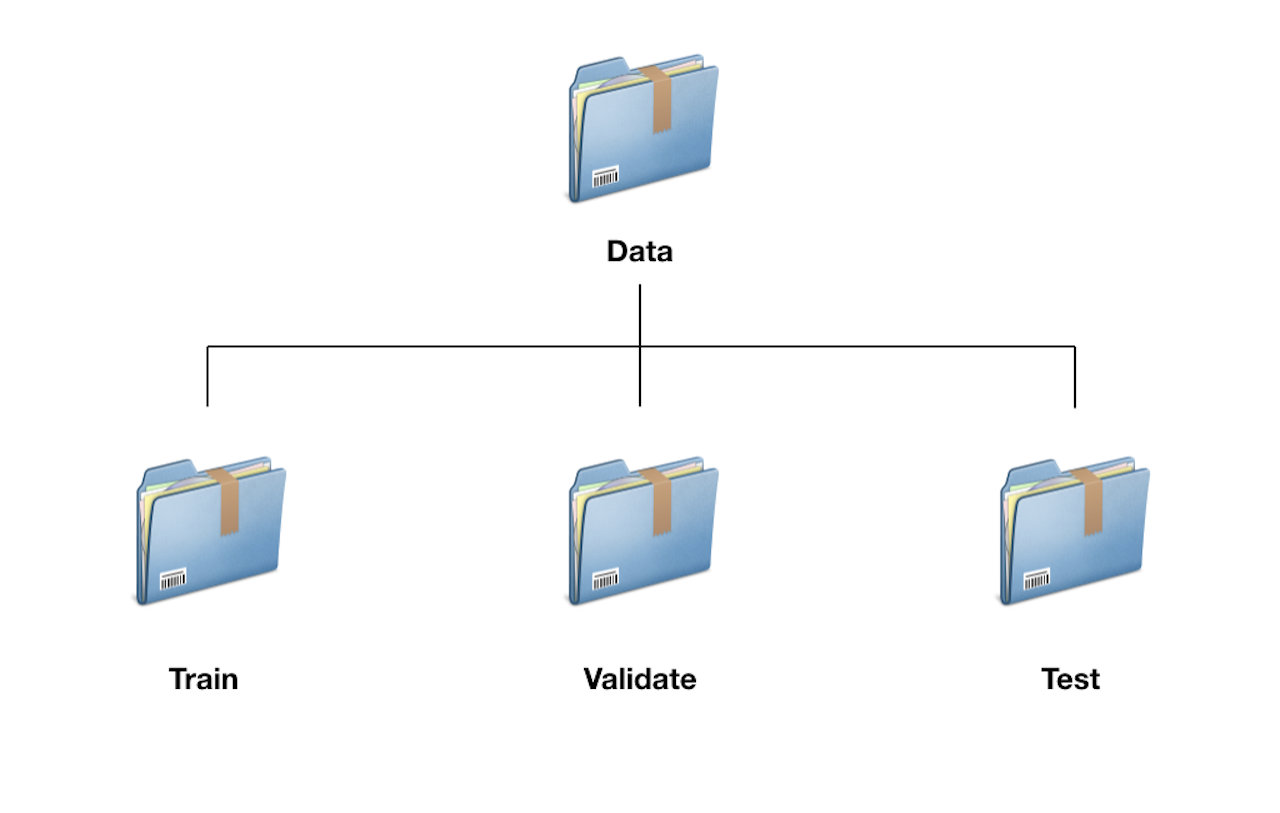
\includegraphics[width=0.75\textwidth]{structure.jpg}
	\caption{Dataset structure}
	\label{fig:datasetstructure}
\end{figure}
%
\subsection{Landing zone dataset}
\label{ssec:landing-zone}
%
The dataset was artificially constructed with a 3D Blender graphics program.(\ref{fig:blender})\\ 
The object of interest are the drone landing mats. These have different shapes
and colors in fact they are available in various color shapes. The signs on
these also vary from the classic H to X to more or less conspicuous symbols.
Thus three models were created, two with a circular plan and one with a square
plan. Textures were then applied to these two models to obtain a faithful
representation of that of concrete objects. \hfill \break
After the construction of the carpet models, it was necessary to contextualise 
them in credible scenarios. \hfill \break
%
\begin{figure}[htb]
	\centering
	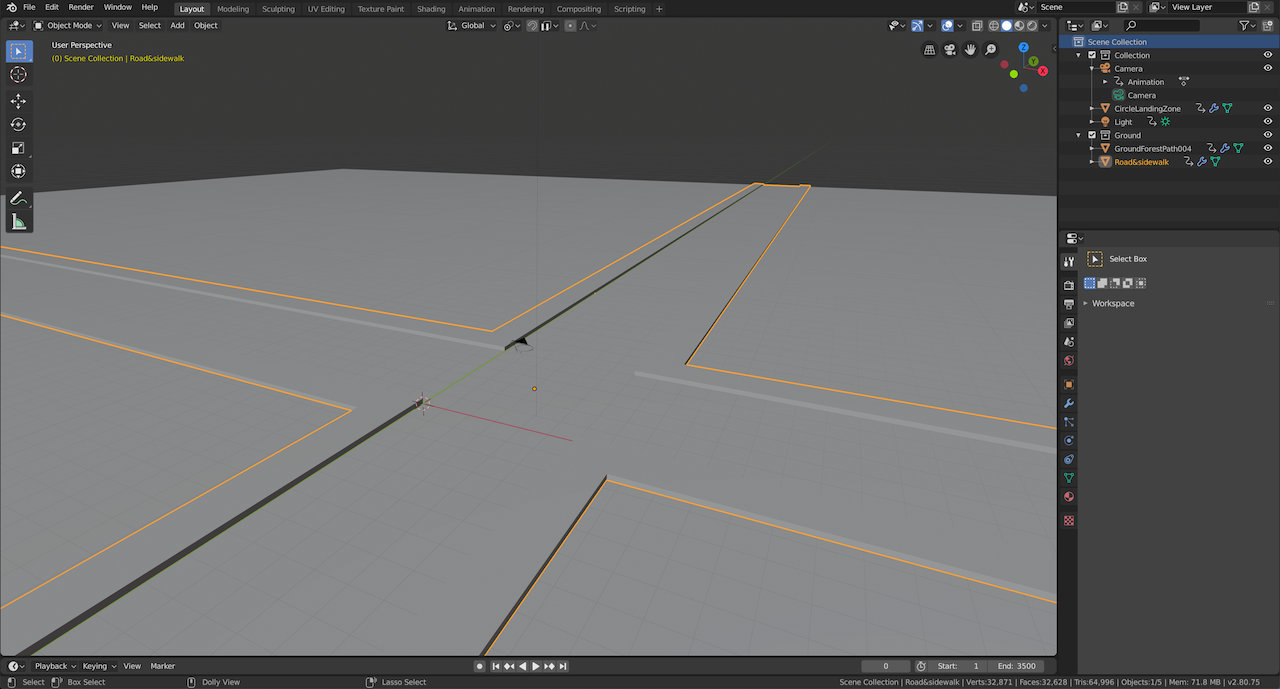
\includegraphics[width=0.75\textwidth]{blender.jpg}
	\caption{Modelling phase of the scenario in Blender.}
	\label{fig:blender}
\end{figure}
%
\\Thus, three main scenarios were created: first scenario placed in the middle of a road
junction. Second scenario near a straight road flanked by a side-walk.
Third zone is set in the countryside. To take the shots, some photographic
factors were taken into account, in fact they are generated starting from the
technical characteristics of the Raspberry camera presented in section
(\ref{sec:raspicam}). Moreover, thanks to a simple script, the trigger points
were generated with respect to the landing mat position, these positions vary in
height, width and depth with respect to the carpet placed on the ground.
A scheme is visible in figures (\ref{fig:poi_dataset}). \hfill \break
%
\begin{figure}[htb]
	\centering
	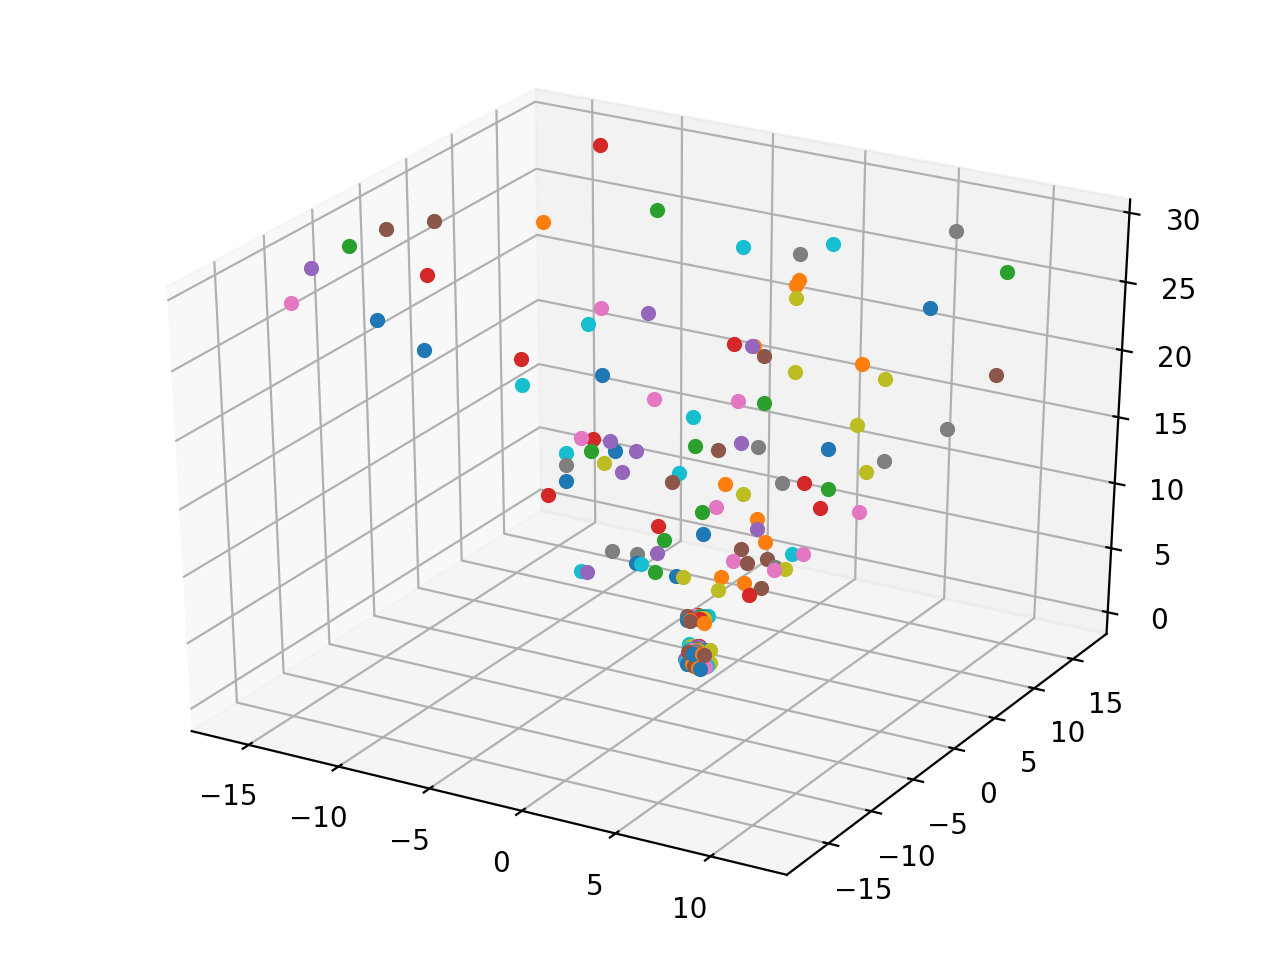
\includegraphics[width=0.75\textwidth]{poi_dataset.jpg}
	\caption{Configuration camera position.}
	\label{fig:poi_dataset}
\end{figure}
%
\newpage
To increase the variety of rendered shots, a very basic day-night cycle was
used to detect the color variation. All the shots are taken with a top view as
seen in the examples shown in (\ref{fig:renders}).
After completing the shots they annotated themselves highlighting the position
of the object of interest in the various shots and positions.
The process is carried out with the aid of a software that extracts and
generates the annotations. as shown in figure (\ref{fig:annotation}).
\begin{figure}[htb]
	\centering
	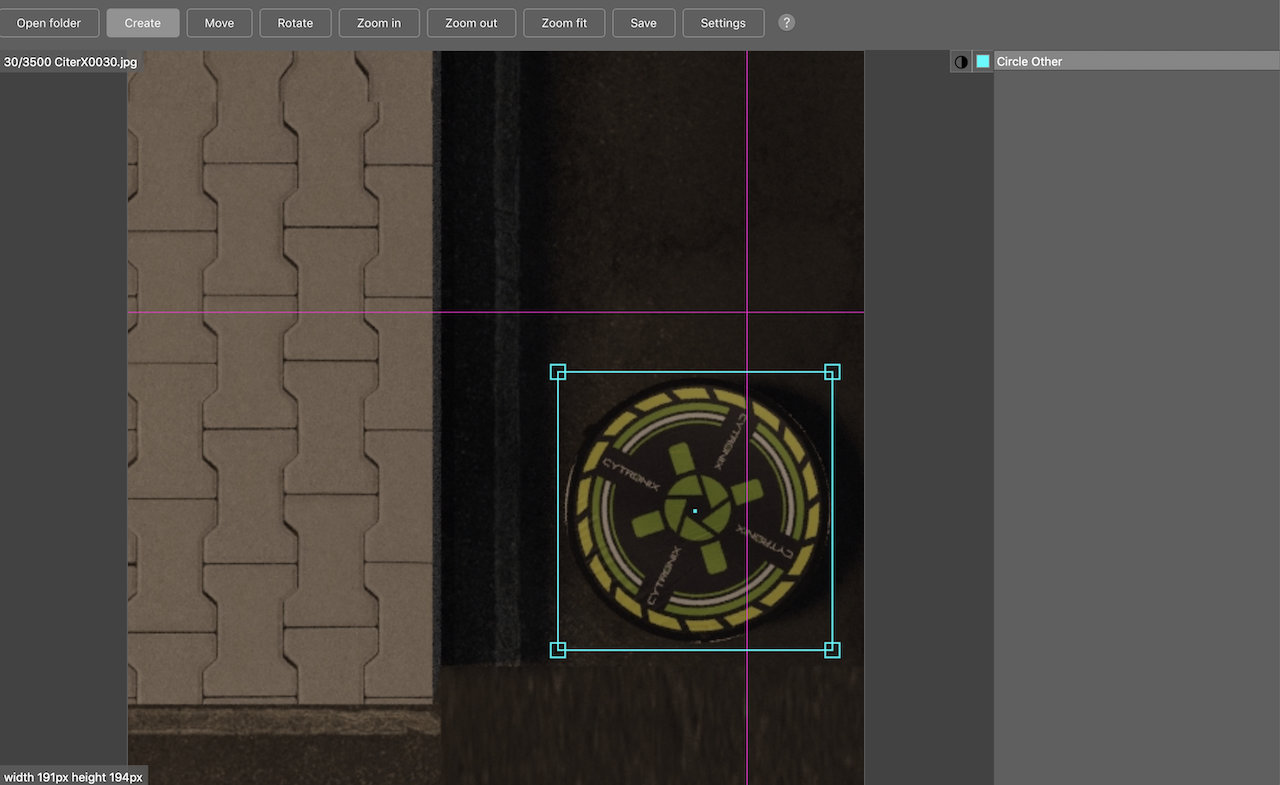
\includegraphics[width=0.70\textwidth]{annotation.jpg}
	\caption{Process of annotation.}
	\label{fig:annotation}
\end{figure}
%
\begin{figure}[htb]
    \centering
    \subfloat[][\emph{middle of a road junction (sunrise)}.\label{subfig:junction}]
        {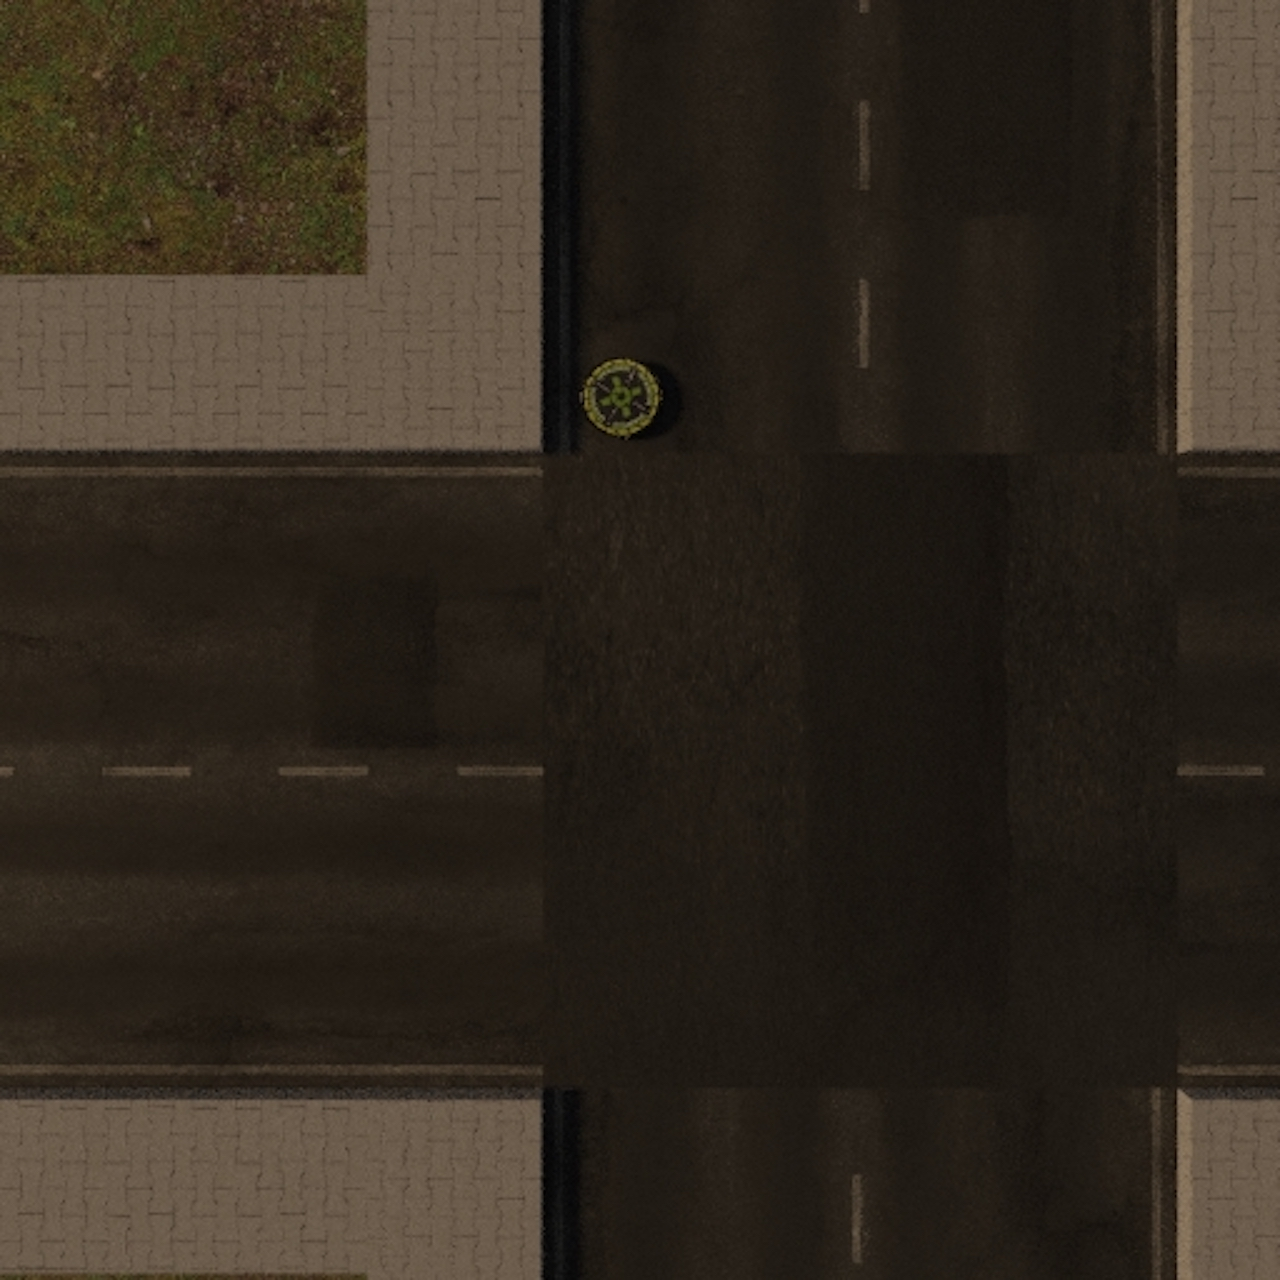
\includegraphics[width=.50\textwidth]{result1.jpg}} \quad
    \subfloat[][\emph{countryside}.\label{subfig:country}]
        {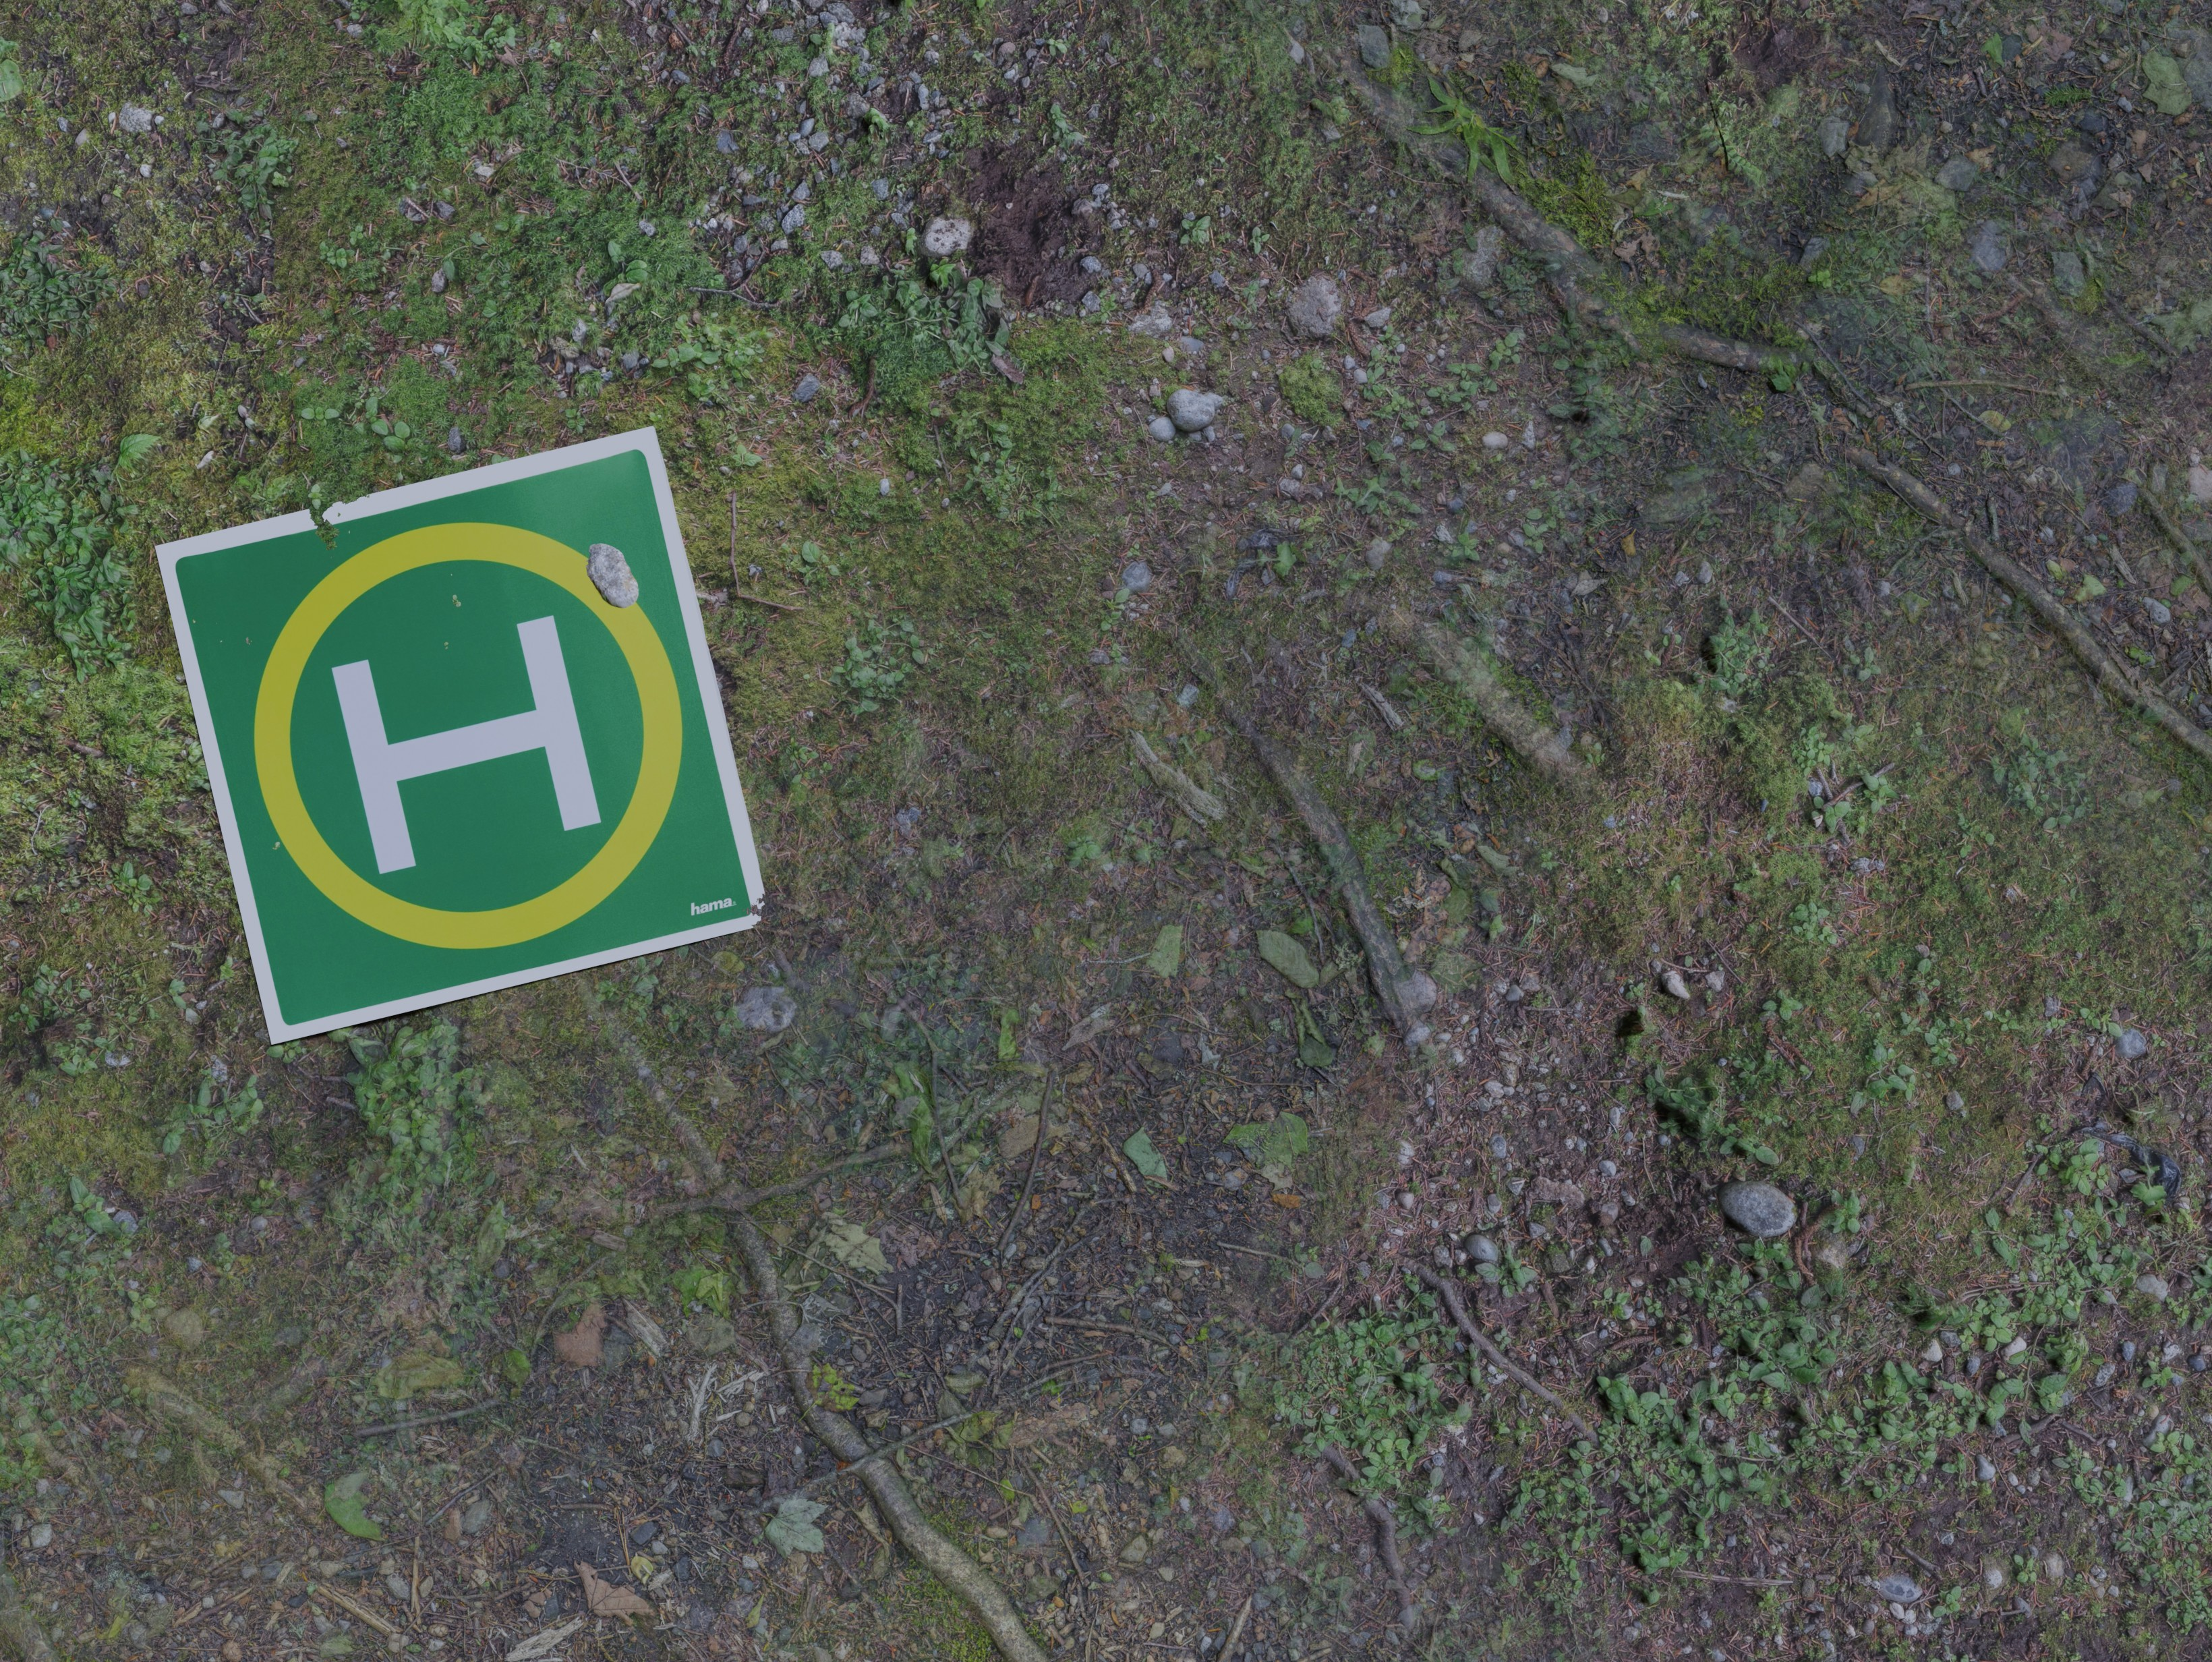
\includegraphics[width=.50\textwidth]{result2.jpg}} \quad
    \subfloat[][\emph{close position at the crossroads}.\label{subfig:junction2}]
        {\includegraphics[width=.50\textwidth]{result3.jpg}}
    \caption{Examples shots scenarios after render}
    \label{fig:renders}
\end{figure}
%
%
\subsection{Thermal imaging dataset}
\label{ssec:thermal-image-dataset}
The dataset created and distributed free of charge by
FLIR\footnote{\href{https://www.flir.com/oem/adas/adas-dataset-form/}{https://www.flir.com/oem/adas/adas-dataset-form/}}
was used to train the neural network on the recognition and classification of
objects in thermal images. The ability to sense thermal infra-red radiation, or
heat, within the ADAS context provides both complementary and distinct
advantages to existing sensor technologies such as visible cameras, LiDAR and
radar systems: With over 15 years of experience in automotive, FLIR has the only
automotive-qualified thermal sensor that is deployed in over 500,000 cars today
for driver warning systems. The FLIR thermal sensors can detect and classify
pedestrians, bicyclists, animals and vehicles in challenging conditions
including total darkness, fog, smoke, inclement weather and glare, providing a
supplemental dataset beyond LiDAR, radar and visible cameras. The detection
range is four times farther than typical headlights. When combined with visible
light data and distance scanning data from LiDAR and radar, thermal data paired
with machine learning creates a more comprehensive detection and classification
system.\cite{flirdataset}\hfill\break
\\The dataset provided by FLIR was created from videos collected from a moving
vehicle in Santa Barbara, California, USA covering roads and highways in
different weather conditions. Although there are many objects in the images to
be catalogued, only ten types of objects have been selected, in particular:
\begin{itemize}
\item Category 1: People
\item Category 2: Bicycles - bicycles and motorcycles (not consistent with coco)
\item Category 3: Cars - personal vehicles and some small commercial vehicles.
\item Category 17: Dogs
\end{itemize}
%
The boxes around the objects of interest are as narrow as possible in fact: when
occlusion occurred, only non-occluded parts of the object were annotated. Heads
and shoulders were favoured for inclusion in the bounding box over other parts of
the body for people and dogs. When occlusion allowed only parts of limbs or
other minor parts of an object to be visible, they were not annotated. 
Wheels were the important part of the Bicycles category.
Bicycle parts typically occluded by riders, such as handlebars, were not included in the bounding box.
People riding the bicycle were annotated separately from the bicycle. When an
object was split by an occlusion, two separate annotations were given to the two
visible parts of the object.
%
\begin{figure}[htb]
    \centering
    \subfloat[][\emph{person}.\label{subfig:th-person}]
        {\includegraphics[width=.50\textwidth]{FLIR_00658.jpeg}} \quad
    \subfloat[][\emph{cars and people}.\label{subfig:th-car}]
        {\includegraphics[width=.50\textwidth]{FLIR_00690.jpeg}} \quad
    \subfloat[][\emph{bicycle and persons}.\label{subfig:th-bycicle}]
        {\includegraphics[width=.50\textwidth]{FLIR_00356.jpeg}}
    \captionsource{Thermal image extracted from FLIR dataset.}{\href{https://www.flir.com/oem/adas/adas-dataset-form/}{https://www.flir.com}}
    \label{fig:th-image}
\end{figure}



%%%%%%%%%%%%%%%%%%%%%%%%%%%%%%%%%%%%%%%%%%%%%%%%%%%%%%%%%%%%%
\section{Data Augmentation Strategies for Object Detection}
\label{sec:nn-augmentation-strategies}
%%%%%%%%%%%%%%%%%%%%%%%%%%%%%%%%%%%%%%%%%%%%%%%%%%%%%%%%%%%%%
	\chapter{Conclusion}
\label{chap:conclusion}
%
% preface chapter
\lettrine[lines=3]{T}{his}

L'obiettivo di questa tesi è aumentare le capacità di automazione e calcolo a
bordo con l'ausilio del machine learnig, in particolar modo risolvendo il
problema comaputer vision ed in particolar modo di object detection.
Il sitema utilizza una telecamera standard con risoluzione da 8 MegaPixels per
acquisire immagini che verrano processate dalla rete neurale, cosi come pone può
fare affidamento sulle tlecamera termica Lepton 2.5 per rilevare oggetti che
emettono calore. In particolare il software realizzato è concepito per sfuttare
al massimo la parallelizzazione del processore, appunto per gestire i flussi
video provienti dalla telecamere. Dispone di una connessione TCP per inviare i
due flussi ad un eventuale dispotivo connesso alla stessa rete.
Così è possibile effettuare direttamente a bordo l'inferenza con il modello
neurale che nel caso di immagini a colori cercherà di indentificare il tappetto
di atterraggio, mentre nel caso della telecamera termica il secondo modello
neurale cercherà di indentificare eventuali ostacoli, in questo caso persone,
per evitarle durante l'esecuzione delle manovre. 
Come discusso l'uso del deep learning permette di risolvere un problema specifico
taradno la risposta su i dati in input per avere in risposta la classificazione
dell'oggetto e la sua posizione del all'interno del frame catturato dalla
fotocamera. In particolare utilizzando il modello di single shot detection
basato su mobilenet, fornisce ottimi risulati sia nella classificazione degi
soggetti inquadrati sia la posizione di bounding box che incornicia il medesimo.
Le tecniche di fine tuning permettono cosi di addestrare in breve tempo il
modello per classificare uno specifico target. Chiaramente questo come è detto
non è possibile farlo a bordo del drone, ma sono necessari dipositivi ad elevate
prestazioni computazioni come il cluster HPC di Ateneo messo a disposizione.
L'uso del framework TensorFlow Lite comprimere il modello una volta addesstrato,
per cui è possibile scegliere su usare valori in virgola mobile o interi. In
particolare modo l'utillizzare un modello compresso permette di essere
utilizzato su dispotivi embedded, tipicamente meno performanti, quali possono
essere computer board card, come ad esempio la Raspberry Pi 3b usata in questo
progetto, fornendo quindi prestazioni accettabili. L'uso invece di processori
dedicati come TPU montato sulla Coral Dev-Board dimostra come ancora sia
possibile aumentare la velocità di risposta del modello neurale grazie
all'utilizzo spinto degli interi a 8-bit. Sebbene siano notevoli i benefici
raggiunti la compressione penalizza il risultato finale a conclusione del
processo inferenza in quanto la grande differenza tra le architetture dei
processori, le ottimizzazioni intordotte dal compilatore e dall'utente
influiscono sul riconoscimento del target producendo così un leggero aumento dei
casi di falsi positivi.
Malgrado sia possibile codificare qualsiasi modello in TensorFlow Lite questo
non è sempre posiibile, infatti utilizzando layer custom possono impedire la
compressione del modello addestrato.
Per questo motivo si è optato ad utilizzare non un modello personalizzato come
all'inizio, ma un modello maggiormente compatibile con TensorFlow Lite e che
presentasse il giusto bilanciamento tra accuratezza e velocità di esecuzione,
questo ha anche garantito la piena compatibilità anche la TPU.
In definitiva è possibile rimarcare che il lavoro qui svolto produce un sistema
in grado di aumentare le capacità di un drone grazie l'ausilio del deep learning
senza ricorrere a soluzione preesistenti derivanti da licenze chiuse o
commerciali abbiante a dispositivi in vendita.
	\chapter{Future work}
\label{chap:future-work}
%
% preface chapter
\lettrine[lines=3]{T}{his}
	% === Bibliografia ====================================
	\newpage
	\bibliographystyle{IEEEtran}
	\bibliography{bibliografia-tesi.bib}
\end{document}
%========================================
